\documentclass[a4, 10 pt, journal]{IEEEtran}
%\bibliographystyle{plain}


%\usepackage{algorithm}
%\usepackage{algpseudocode}
\usepackage{amsmath}
\usepackage{amssymb}
%\usepackage{appendix}
\usepackage[backend=bibtex,style=ieee,sorting=nty]{biblatex}
\usepackage{bm}
\usepackage{cancel}
\usepackage{caption}
\usepackage{colortbl}
%\usepackage{flafter}
\usepackage{float}
\usepackage{flushend}
\usepackage{fontawesome}
\usepackage{fourier}
\usepackage{geometry}
\usepackage{graphicx}
\usepackage{hyperref}
\usepackage[utf8]{inputenc}
\usepackage{lipsum}
\usepackage{makecell}
\usepackage{mathtools}
\usepackage{multicol}
\usepackage{multirow}
\usepackage[section]{placeins}
\usepackage{subfig}
%\usepackage{subcaption}
\usepackage{soul}
\usepackage{tcolorbox}
\usepackage{tikz}
\usepackage{units}
\usepackage{url}
\usepackage{wrapfig}

\graphicspath{ {./fig/} }

\DeclareMathAlphabet{\mathcal}{OMS}{cmsy}{m}{n}
\DeclareUnicodeCharacter{0301}{\hspace{-1ex}\'{ }}
\newtheorem{assumption}{Assumption}
\newtheorem{definition}{Definition}
\newtheorem{axiom}{Axiom}
 \geometry{
     a4paper,
     total={170mm,257mm},
     left=20mm,
     top=20mm,
 }
 
%\include{variables.tex}

\usetikzlibrary{backgrounds}
\makeatletter

\tikzset{%
	fancy quotes/.style={
		text width=\fq@width pt,
		align=justify,
		inner sep=1em,
		anchor=north west,
		minimum width=\linewidth,
	},
	fancy quotes width/.initial={.8\linewidth},
	fancy quotes marks/.style={
		scale=8,
		text=white,
		inner sep=0pt,
	},
	fancy quotes opening/.style={
		fancy quotes marks,
	},
	fancy quotes closing/.style={
		fancy quotes marks,
	},
	fancy quotes background/.style={
		show background rectangle,
		inner frame xsep=0pt,
		background rectangle/.style={
			fill=gray!25,
			rounded corners,
		},
	}
}

\newenvironment{fancyquotes}[1][]{%
	\noindent
	\tikzpicture[fancy quotes background]
	\node[fancy quotes opening,anchor=north west] (fq@ul) at (0,0) {``};
	\tikz@scan@one@point\pgfutil@firstofone(fq@ul.east)
	\pgfmathsetmacro{\fq@width}{\linewidth - 2*\pgf@x}
	\node[fancy quotes,#1] (fq@txt) at (fq@ul.north west) \bgroup
}
{\egroup;
	\node[overlay,fancy quotes closing,anchor=east] at (fq@txt.south east) {''};
	\endtikzpicture}

\makeatother
\newcommand\myhl[1]{\textcolor{red}{#1}}
\newcommand*{\important}[1]{\textcolor{red}{\danger~\textbf{IMPORTANT:~} #1}}
\newcommand{\task}{\ensuremath{\tau}}
\newcommand{\sltwoi}{\ensuremath{t_l}} %single learning time without index
\newcommand{\slt}[1]{\ensuremath{t_{l,#1}}} %... with index
\newcommand{\tlt}{\ensuremath{T}} %total learning time
\newcommand{\comp}{\ensuremath{c}} %complexity (learning time from scratch)
\newcommand{\diste}[1]{\ensuremath{\mathrm{d}(\task_{#1},\{ \})}}
\newcommand{\dist}[2]{\ensuremath{\mathrm{d}(\task_{#1},\{\task_1, \task_2, \dots, \task_{#2}\})}}
\newcommand{\En}{\ensuremath{E}}
\newcommand{\opt}{\ensuremath{\mathrm{opt}}}
\newcommand{\tot}{\ensuremath{\mathrm{tot}}}
\newcommand{\Opt}{\ensuremath{\mathrm{Opt}}}
\newcommand{\densMan}{\ensuremath{\rho_{\mathrm{man}}}} %manufacturing energy density
\newcommand{\Tau}{\ensuremath{\mathcal{T}}}
\newcommand\mybox[2][]{\tikz[overlay]\node[fill=blue!100,inner sep=4pt, anchor=text, rectangle, rounded corners=1mm,#1] {#2};\phantom{#2}}
\newcommand{\TODO}{\mybox[fill=yellow]{\textcolor{blue}{\Large \textbf{TODO}}}}

\setlength{\columnsep}{1cm}

\newtheorem{challenge}{\textbf{CHALLENGE}}

\addbibresource{bib/References.bib}


\hypersetup{draft}
\begin{document}
\pagestyle{empty}
%\title{On the relation between learning model and knowledge transfer for a sustainable energy balance in embodied AI}
\title{Knowledge sharing as the key to a sustainable energy balance in embodied AI}

\author{Fernando D\'iaz Ledezma and Sami Haddadin$^{1}$%\vspace{-1ex}
\thanks{$^{1}$ {\small \{fernando.diaz, haddadin\}@tum.de}, 
Both authors are with the Chair of Robotics and Systems Intelligence, MIRMI - Munich Institute of Robotics and Machine Intelligence, Technical University of Munich (TUM), Munich, Germany}}
\date{March 2023}
%\maketitle

\twocolumn[
  \begin{@twocolumnfalse}
    \maketitle
  \end{@twocolumnfalse}
]

% ***************************************************************************************************
 \begin{abstract}
Classical AI and its current learning paradigms require copious amounts of energy due to their high computational loads and subpar exploitation of the acquired knowledge. As AI and robotics progressively integrate to form embodied AI (EAI) systems, their energy demand will continue to increase as data acquisition and learning rely on constant and active interaction with the physical environment. In this work, we look at the basic energetic demands of embodied AI systems and discuss the growing energetic challenges that will arise if the current learning paradigms are maintained. Consequently, using an energy estimation model, we argue that collective learning, a paradigm shift that departs from isolated learning and expands on the concepts of transfer and incremental learning, is the proper way for embodied AI agents to learn new skills as it shares and actively uses previous and current knowledge across systems to learn more skills in shorter time needing considerably less energy.
 \end{abstract}
% ***************************************************************************************************

% ===================================================================================================
%                                                 |                                                 |
%                                                 |                                                 |
% -------------------------------------------- SECTION ---------------------------------------------|
%                                                 |                                                 |
%                                                 |                                                 |
% ===================================================================================================
% ===================================================================================================
%                                                 |                                                 |
%                                                 |                                                 |
% -------------------------------------------- SECTION ---------------------------------------------|
%                                                 |                                                 |
%                                                 |                                                 |
% ===================================================================================================
\section{Introduction}\label{sec:intro}
%---
\begin{fancyquotes}
	AI is one of the cornerstones of the growing digitization of industry ('Industry 4.0'). Technologies underpinning  this  process  ---  such as IoT,  5G,  \textbf{cloud  computing},  big  data  analytics,  \textbf{smart  sensors},  augmented  reality,  3D  printing  and  \textbf{robotics}  ---  are  likely  to  transform  manufacturing  into  a  single cyber-physical  system  in which digital  technology,  internet  and  production  are merged in one \cite{szczepanski_2019}.
\end{fancyquotes}
%---
\textcolor{red}{As technology develops, not only smart factories will become the norm, but healthcare services modernize and households evolve into mostly automated environments. Modern industrial, cooperative, service, and healthcare robots with local and network computing capabilities would populate these environment, collecting and sharing data from their various sensors.} AI will be a natural component of these robots, enabling them to learn new skills and spread their acquired knowledge across systems. The more these \emph{embodied AI} (EIA) agents integrate synergistically into these varied environments, the more they will take over diverse tasks while also actively cooperating with humans. Yet, as EAI agents become ubiquitous, new challenges will emerge, among them, their energy demand.

% SUBSECTION ========================================================================================
\subsection{The energy problem in classical and embodied AI}
Classical AI interprets intelligence as a purely computational symbol-processing problem decoupled from physical agents. Progress in classical AI relies on two computing stages: (i) learning and (ii) deployment. While the latter is not energy-efficient compared to its biological counterparts, the former craves a large energy quota to process large amounts of data for training, validation, and testing of models (e.g., supercomputing). Furthermore, both model and training data are expected to carry enough information to transfer knowledge between different tasks and even systems (at least to a certain extent). However, retraining is required when this information is unavailable in the data ---sometimes even from scratch---, leading to highly energy-inefficient learning paradigms. The implication is that the energetic cost of classical AI can sometimes outweigh the benefits \cite{Strubell2019EnergyAP}. \textcolor{red}{Even mayor breakthroughs like the use of transformer models for Natural Language Processing come with its energetic challenges\cite{Cao2020TowardsAccurateReliable}.}

With the evolution towards embodied AI systems, i.e., the emerging field between AI and robotics, the challenges mentioned before expand. Since the real world cannot be faithfully replicated in virtual environments, and in spite the considerable advances in sim-to-real applications \cite{Chebotar2019Closingsimreal}, data acquisition in EAI agents necessitates constant and active energy-expending interaction with the physical environment. Likewise, in the real world, learning a skill implies physically executing it, and with each execution, energy is required for motion and interaction. Consider, for example, autonomous driving, where the vehicle is a rather rudimentary form of an EAI agent. Despite operating primarily in a structured human-made environment, complexity is already present in the system, as the vehicle spends energy simply by carrying out its purpose: autonomous movement; but also spends energy by collecting vast amounts of data (obtained by driving around) to retrain and improve the policy model. \textcolor{red}{Household robots are another example, current estimates indicate that 39\% of the domestic chores could be automated in the short term \cite{Lehdonvirta2022futuresunpaidwork}. Yet, even when compared to factory floors, homes still represent challenging dynamic environments that require EAI agents to undergo constant retraining.} While the energy demand of AI and robotics entered the scope of separate research communities in the last few years, the study of the energetic requirements of embodied AI and its vast implications has not received proper attention. 
% ---
\begin{figure*}[!t]
	\centering
	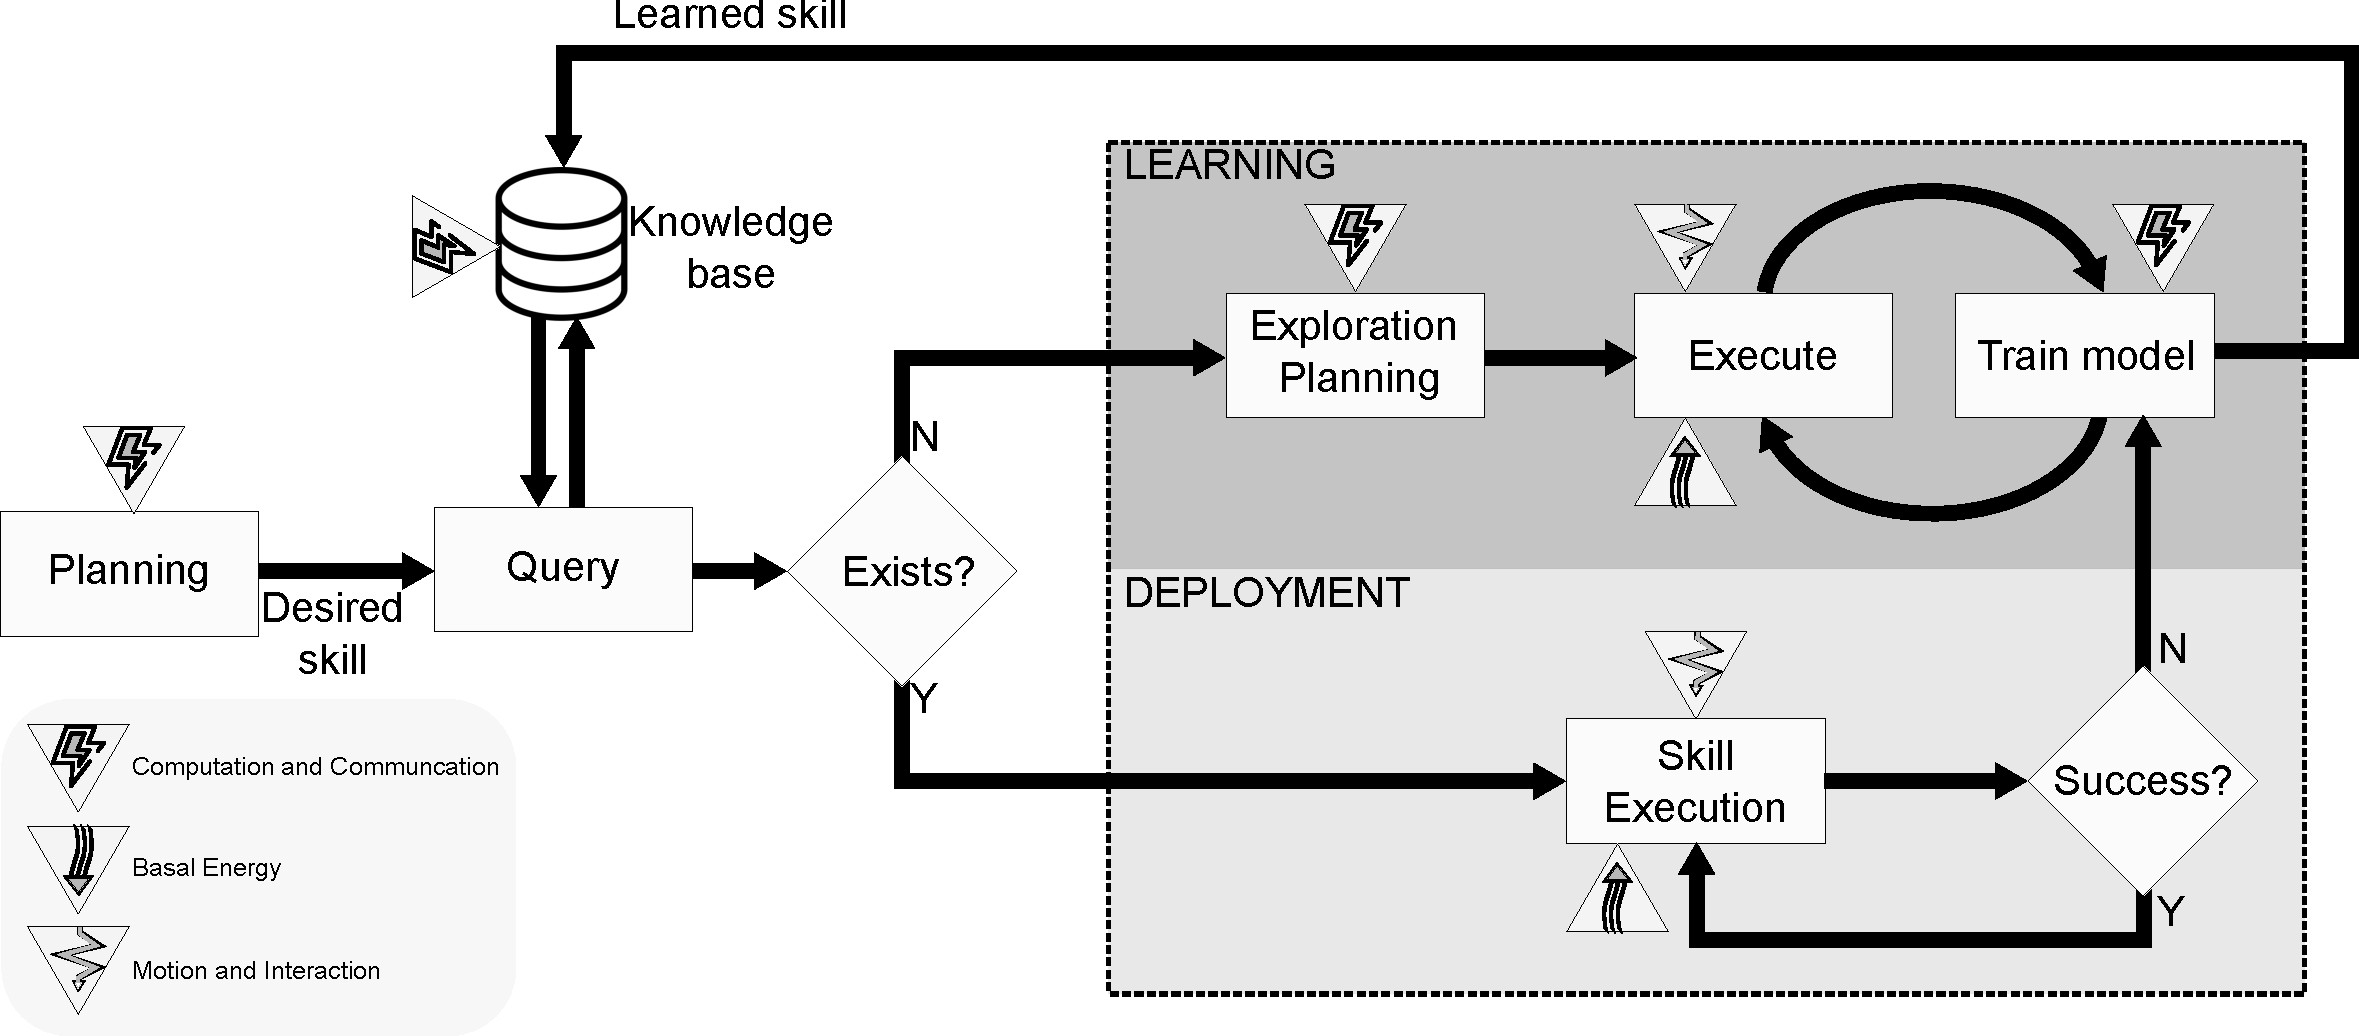
\includegraphics[width=0.9\textwidth]{fig/embodied_ai_learning_pipeline_v7.pdf}
	\caption{Standard skill execution pipeline of isolated EAI agents.}
	\label{fig:embodied_ai_pipeline}
\end{figure*}
% ---
% SUBSECTION ========================================================================================
\subsection{Contributions}
To facilitate the study of the energetic demand of EAI agents, we look at the standard skill execution pipeline of an isolated agent, shown in Fig.~\ref{fig:embodied_ai_pipeline}, and identify three main categories of energy usage, namely
% ---
\begin{enumerate}
	\item Computation and Communication Expenditure (CCE): Refers to the energy required by the computation process itself (e.g., the number of floating point operations) and by the supporting communication processes
	\item Basal Energy Expenditure (BEE): This is the energy associated with the basic functions of the EAI agent. For example, gravity compensation and proprioceptive intelligence/algorithms in robots, hovering in drones, running on-board system standby in autonomous vehicles, etc.
	\item Motion and Interaction Expenditure (MIE): Defines the energy spent on executing a particular skill in a certain form
\end{enumerate}
% ---
Consequently, we provide projections on the growing energetic challenges in embodied AI pertaining to these categories and show that the energy demand scales out of proportion with the number of EAI agents if learning paradigms that do not promote and systematically exploit knowledge exchange persist. Furthermore, we establish that with the scaling complexity of the problems faced by classical and embodied AI, clever learning methods are required that not only make efficient use of the computation and physical power of the embodied agent but also leverage modern communication infrastructure to optimally collect, share, and transfer the knowledge acquired by other agents performing similar skills. For this, we contextualize the problem in a hypothetical case study using empirical/reported energy consumption estimations and introduce a full energy estimation model that accounts for the three energy expenditure categories (CCE, BEE, and MIE). Concretely, we estimate the substantial effect that our recently introduced paradigm of \emph{collective learning} can have on energy and time-saving components in a smart factory scenario with many robots performing many skills. We show that collective learning is the natural solution to address the energy problem in embodied AI.

% SUBSECTION ========================================================================================
\subsection{Paper organization}
The remainder of this work is arranged as follows. In Sec.~\ref{sec:energy_demand_embodied_ai}, we discuss the energy demands brought about by the two main components of embodied AI: machine learning algorithms and robotics. Consequently, in Sec.~\ref{sec:energy_grand_challenges}, three grand challenges accompanying EAI systems in the context of their energy consumption are introduced. A brief mathematical formulation of the energy and time requirements of four learning paradigms employed with EAI agents is presented in Sec.\ref{sec:learning_paradigms} and used in Sec.~\ref{sec_use_case} in a use-case related to a smart factory to contrast these requirements against each other. Finally, in Sec.~\ref{sec:conclusion}, we summarize the paper and provide conclusions regarding the importance of knowledge sharing and transfer among EAI agents.  

% ===================================================================================================
%                                                 |                                                 |
%                                                 |                                                 |
% -------------------------------------------- SECTION ---------------------------------------------|
%                                                 |                                                 |
%                                                 |                                                 |
% ===================================================================================================
% ===================================================================================================
%                                                 |                                                 |
%                                                 |                                                 |
% -------------------------------------------- SECTION ---------------------------------------------|
%                                                 |                                                 |
%                                                 |                                                 |
% ===================================================================================================
\section{Energy demand of Embodied AI}\label{sec:energy_demand_embodied_ai}
The benefits embodied AI will bring about as it permeates many areas such as the smart factory, healthcare services, and people's, will take a toll, particularly on the energy demand. We briefly go over some of the few recent works that have looked at this issue and that focus on either of the two most relevant components of embodied AI: machine learning and robotics, with the former directly connected to the CCE energy usage category and the latter corresponding to the BBE and MIE categories.

% SUBSECTION ========================================================================================
\subsection{Energy demand in machine learning}
Recently, there has been an increasing concern in the research community about the negative impact of artificial intelligence and machine learning on the environment. For instance, works such as \cite{schwartz2019green}, \cite{vinuesa2020role}, and \cite{Strubell2019EnergyAP} discuss the efficiency of computation-intensive deep learning algorithms\footnote{Consider that the number of computations required by deep learning algorithms has increased more than 300000x in the last decade \cite{schwartz2019green}.} --- such as natural language processing (NLP) --- and express their impact on the environment based on the carbon footprint left by the worldwide data centers used to train and run them. Related works have defined metrics to assess the energy consumption of machine learning algorithms, such as the energy efficiency of their development phases \cite{zhou2020hulk},  the accuracy, model size, time, and CPU/GPU energy consumption for the training and inference phases \cite{Dalgren2019GreenMLA}, as well as other system level performance counters (PMC) like real-time, instruction-level, and a hardware-level power estimation \cite{garcia2019estimation}. Despite this rising awareness about energy consumption in AI, actions are yet to be taken to understand the roots of the problem and present potential solutions to alleviate it.

% SUBSECTION ========================================================================================
\subsection{Energy demand in robotics}\label{sec:energy_in_robotics}
Recent statistics \cite{IFR2019} shows a clear upward trend in the worldwide demand for industrial robots. Such a trend directly links to a significant increase in electric energy consumption. For instance, although focused only on the robotics market in the United States, the study in \cite{barnett_2017} projects that 22,822 GWh will be demanded by the ever-increasing introduction of robots in many aspects of human life. Yet, although the reduction of the energy consumption from industrial robots has been studied in some works \cite{schroder2014, chalmers2015, mohammed2014, chemnitz2011} providing alternatives to make robots more energy efficient ---e.g., exploiting robots with elastic actuation \cite{scalera2019natural, carabin2017review, bolivar2017general, haddadin2011optimal,haddadin2012intrinsically} or methods for better hardware selection and storage and sharing of energy and optimized motion planning \cite{carabin2017review}---,  there is still no precise estimate of the energy demand rise that the increasing number of robot installations will bring into the picture nor a strategy to address this problem.

However, a holistic understanding of the energy challenges arising from the advent of embodied AI still needs to be provided. We attempt to contribute to this understanding by elaborating on these challenges and positioning the recent paradigm of collective learning \textbf{\textcolor{red}{REF TO SIBLING PAPER}} as the core strategy that can leverage scalability and knowledge exchange to achieve energy efficiency in embodied AI.

% ===================================================================================================
%                                                 |                                                 |
%                                                 |                                                 |
% -------------------------------------------- SECTION ---------------------------------------------|
%                                                 |                                                 |
%                                                 |                                                 |
% ===================================================================================================
% ===================================================================================================
%                                                 |                                                 |
%                                                 |                                                 |
% -------------------------------------------- SECTION ---------------------------------------------|
%                                                 |                                                 |
%                                                 |                                                 |
% ===================================================================================================
\section{Energy grand challenges in embodied AI: perspective and research directions}\label{sec:energy_grand_challenges}
Based on the energy expenditure categories introduced in Sec.~\ref{sec:intro}, we have identified three grand energy demand challenges in embodied AI. We discuss them individually in the following, highlighting their implications on future energy consumption.

% SUBSECTION ========================================================================================
\subsection{\textbf{CHALLENGE 1} (C1). Energy for AI infrastructure}
%This challenge is directly connected to the computation and indirectly related to the motion/interaction energy demands depicted in Fig.~\ref{fig:embodied_ai_pipeline}.
Most state-of-the-art machine learning algorithms depend on significant volumes of data or a vast number of computational iterations to converge to a solution \cite{Strubell2019EnergyAP}. To accelerate the time spent training such models, researchers and companies take advantage of the readily available infrastructure or use several cloud computing services running on data centers. A new analysis estimates that data center workloads have increased more than sixfold since 2010. That year, they consumed roughly 194 terawatt-hours (TWh) of energy or 1 \% of worldwide electricity use. Data-center energy use grew just 6 percent to 205 TWh. Fig. \ref{fig:dataCenterEnergy} illustrates the increasing trend in the energy demand from data centers.
%---
\begin{figure}[!t]
	\centering
	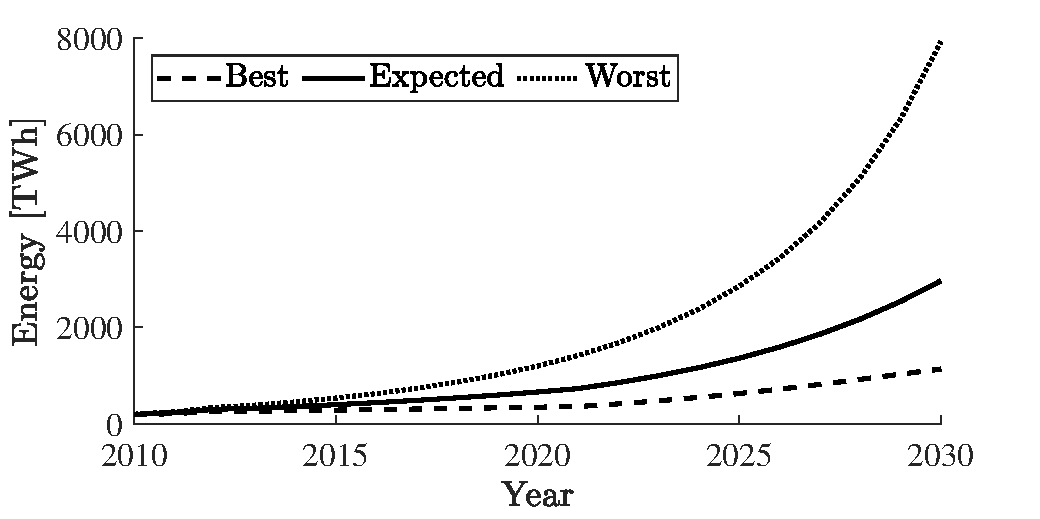
\includegraphics[width=0.9\columnwidth]{fig/data_center_energy_consumption.pdf}
	\caption{Global electricity demand of data centers (adapted from \cite{andrae2015global})}
	\label{fig:dataCenterEnergy}
\end{figure}
% ---
As shown in \cite{Strubell2019EnergyAP}, reference state-of-the-art machine learning algorithms require an incredible amount of computations, especially those requiring constant retraining and re-evaluation, such as neural architecture search \cite{real2019regularized}. A key contribution to increasing the energy consumption of machine learning algorithms emerged because recent techniques allowed data sample complexity to increase from precisely located sensor measurements to full camera images, scaling up the number of computations required in a given architecture iteration \cite{krizhevsky2012imagenet}. The challenge now is to research algorithms capable of reducing the average energy demand despite the increase in processing complexity of the sensory data.

% SUBSECTION ========================================================================================
\subsection{\textbf{CHALLENGE 2} (C2). Energy for the masses}\label{sec:robots_challenge}
As mentioned earlier in Sec.~\ref{sec:energy_in_robotics}, the numbers of robots in service keep increasing. The advent of Industry 4.0 and the smart factory will accentuate this trend, as does the increasing use of robots in service applications. In spite of better robotic systems with improved energy efficiency, analysis tends to focus on individual systems with the aggregate effect of all the active units usually escaping attention. Said succinctly, \emph{more robots, more energy demand}. %In this section we elaborate on this claim and discuss its implications on the global energy landscape.

% ---------------------------------------------------------------------------------------------------
\subsubsection{Industrial robots}
In the last years, the install base of industrial robots has gone from 1,235,389 units in 2012 to an estimate of 3,152,000 units in 2020; signifying a 250 \% increase in only eight years. According to the International Federation of Robotics, the yearly growth has been between 12-15 \% since 2012 \cite{IFR2019}. Based on this rate an astonishing four million robots are estimated to be currently operating in factories around the world. Fig.~\ref{fig:ir_stock} projects this trend until 2025, showing that the install base of industrial robots will be almost three times larger than 2015\footnote{These numbers are in the neighborhood of a slightly more conservative prediction for the robot operational stock presented by \textit{The Boston Consulting Group} in \cite{sirkin2015}.}. Using this projection, and assuming 24/7 operation, we estimate the expected energy demand of industrial robots, i.e., the total \textit{World Robot Energy Consumption} (WREC)\footnote{To determine an estimate of the electric energy consumption derived from the worldwide operational stock of industrial robots, the market distribution per manufacturer was considered as well as an estimate of the average power consumption according to the robot's category (e.g. assembling, processing, welding, etc.). Further details can be found in Appendix~\ref{sec:app_robot_ener_consumption}.}, see Fig.~\ref{fig:ir_energy}. For reference, the WREC in 2025 represents 7.2 \% of the installed electricity generation capacity in Germany (one of the leading industrialized nations) \cite{fraunhofer2016}. 

% ---------------------------------------------------------------------------------------------------
\subsubsection{Collaborative robots and service robots}
Just as industrial robots, the future impact of collaborative and service robots must not be disregarded. As an example, collaborative robots (cobots) jumped from representing only 6 \% of the market in 2017 to about one quarter of the installed base today, see Fig. \ref{fig:industrial_cobot_share} \cite{tobe2015}. Using similar assumptions as for industrial robots, Fig.~\ref{fig:cobot_stock} and \ref{fig:cobot_energy} show the expected growth and corresponding energy consumption for this class of robots. Similar to cobots, service robots are \textit{booming}. The IFR estimated, for example, that the sales of privately used service robots increased to around 35 million units in 2018 \cite{IFR2015}. Applied to a diverse variety of fields including, but not limited to, logistics, defense, public relations, medical applications, etc.; the numbers of service robots exhibit the same increasing trend as industrial and collaborative robots.
%---
\begin{figure}[!t]
	\centering
    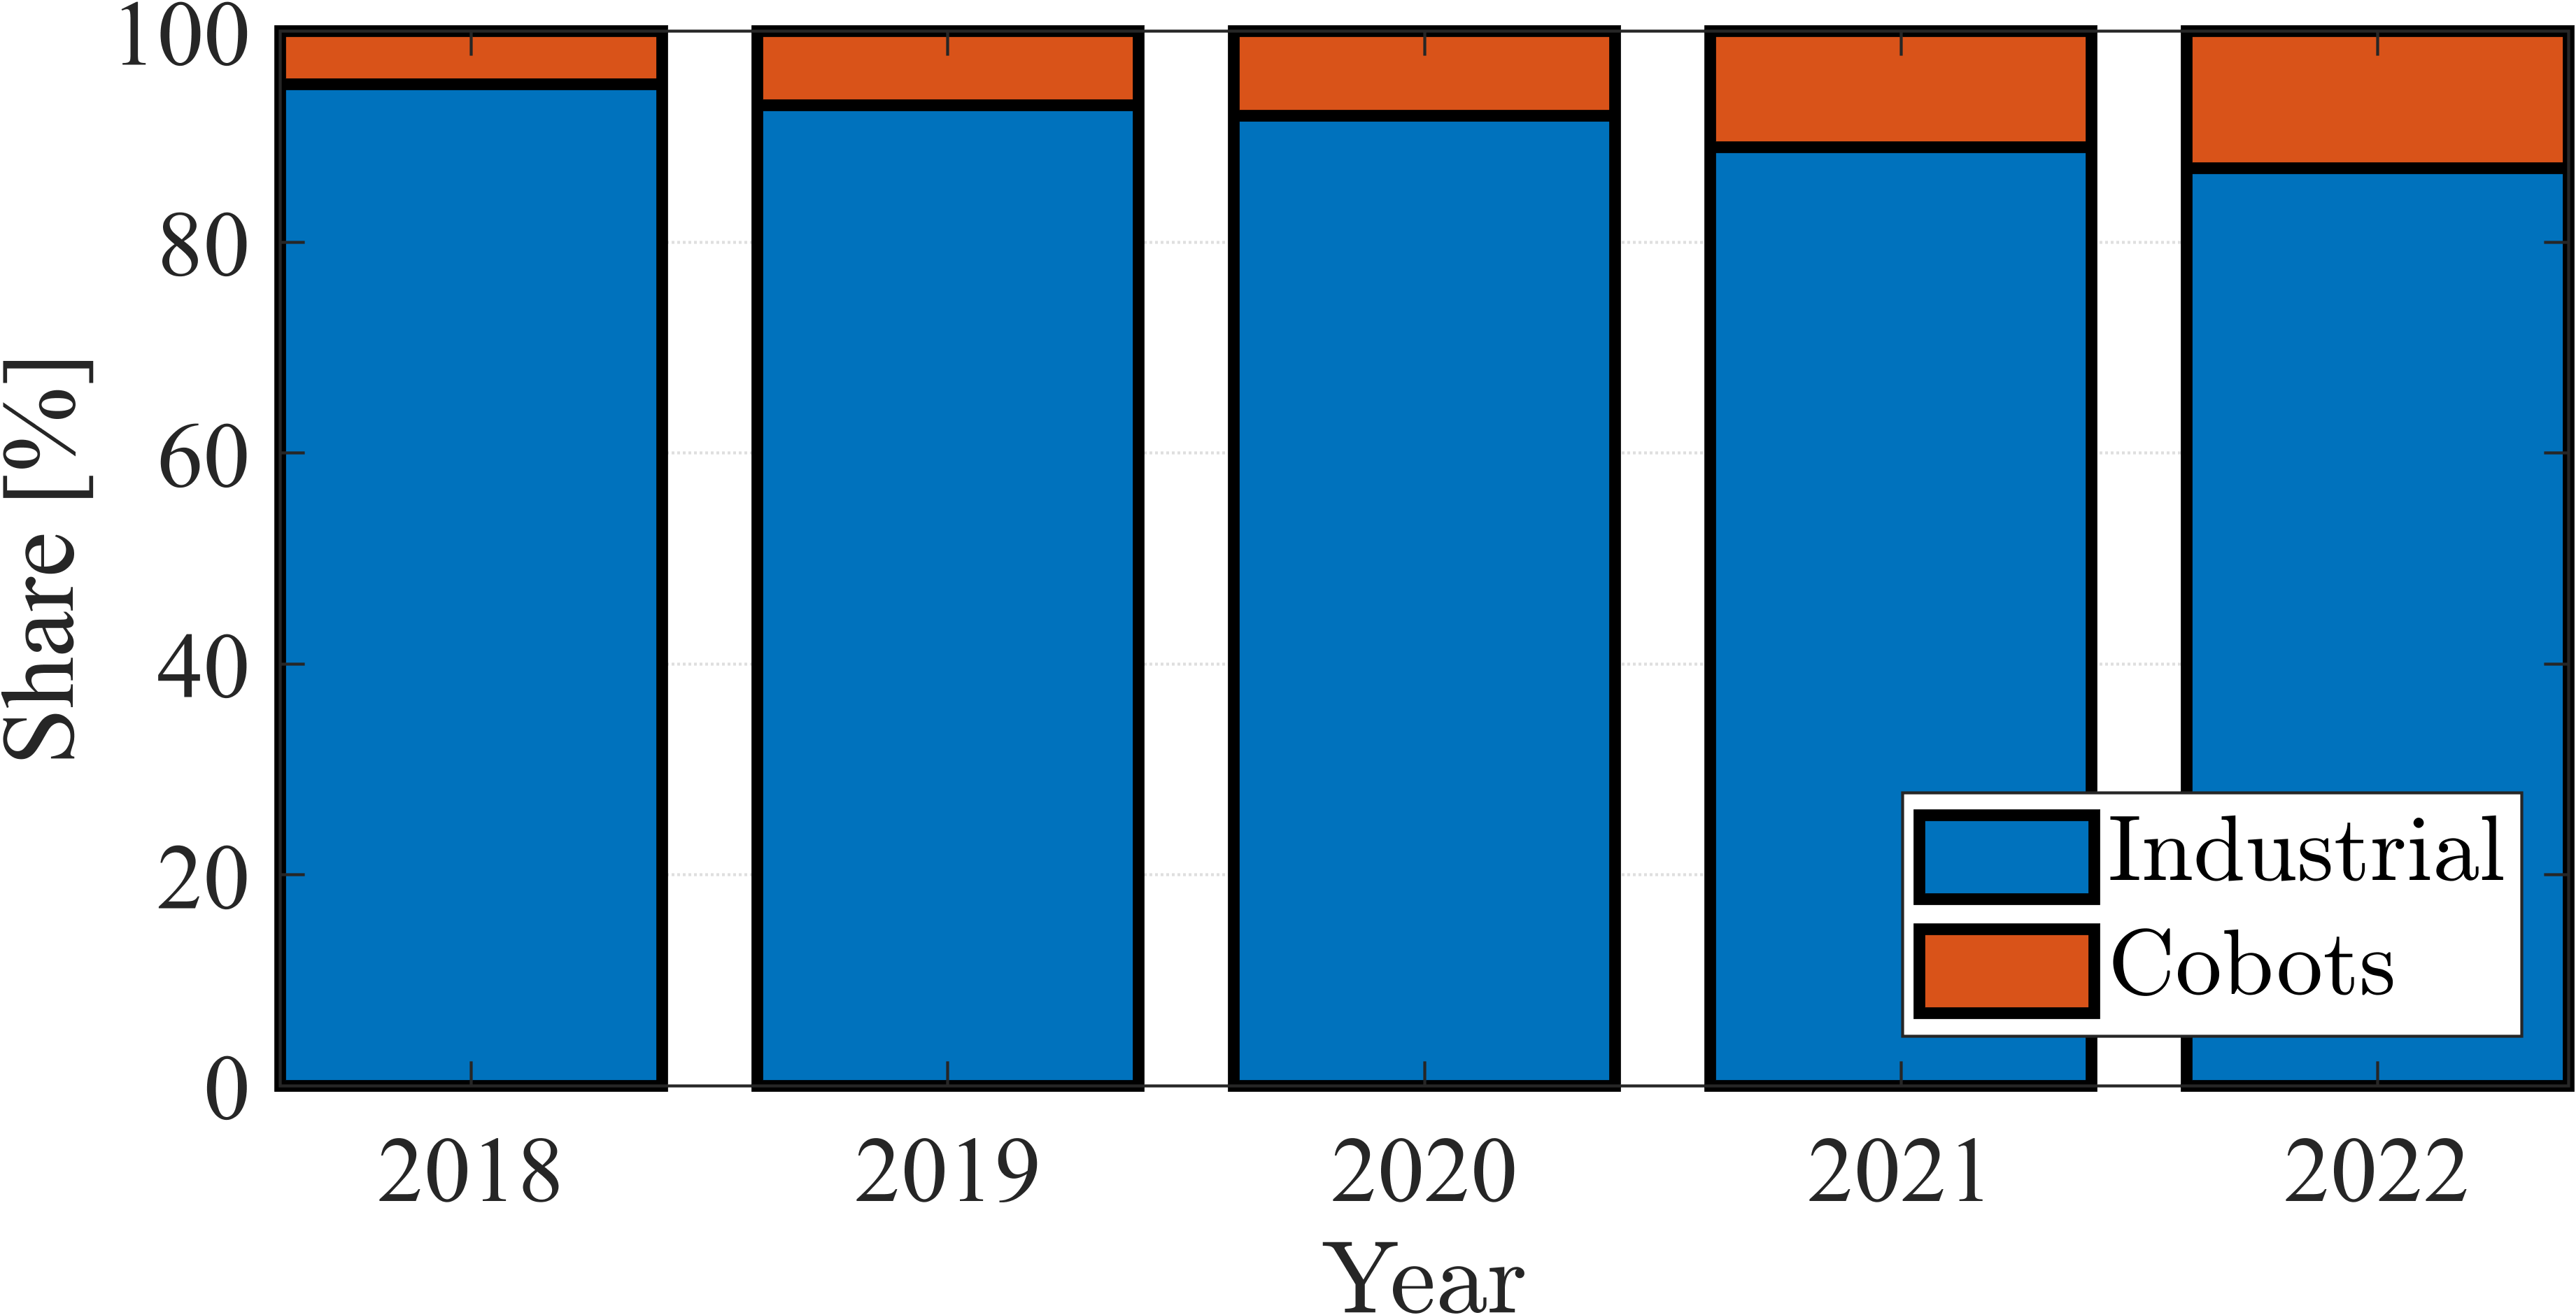
\includegraphics[width= 0.9\columnwidth]{fig/share_industrial_and_cobots} 
	\caption{Ratio of industrial robots to cobots \cite{statista_ir_cobot_share}}
    \label{fig:industrial_cobot_share}
\end{figure}
% ---
% ---------------------------------------------------------------------------------------------------
\subsubsection{Implications}
Modern production paradigms and lifestyle and societal needs will make robots ubiquitous, permeating many aspects of human life. As a consequence, just by their sheer number, industrial, collaborative, and service robots already represent a currently disregarded niche in the global energy landscape. In standard operation, the energy they consume corresponds naturally to the BEE and MI categories in embodied AI systems and thus, the numbers introduced in this section serve as an indication of the base energetic requirements in embodied AI. Concretely, the challenge here consists on devising better strategies for the efficient use of these legions of robots. That is, if the skills that these robots take care of are performed in the most time and energy optimal fashion then BEE and MI energies will also be kept at the optimal minimum.
%---
\begin{figure*}[!t]
	\centering
% 	\hspace*{\fill}
% 	\subfloat[]{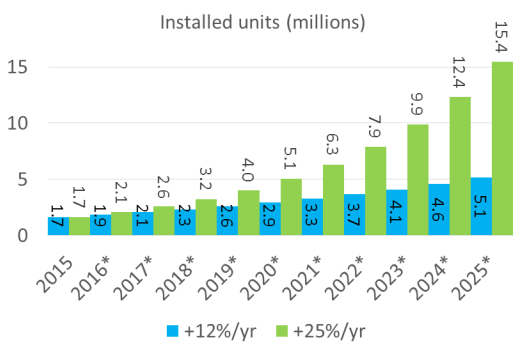
\includegraphics[width= 0.90\columnwidth]{fig/robot_stock} \label{fig:ir_stock}}
% 	\hfill
% 	\subfloat[]{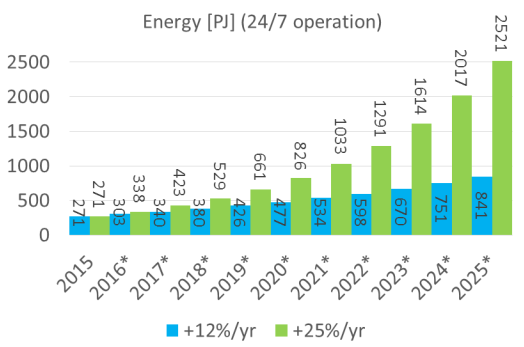
\includegraphics[width= 0.90\columnwidth]{fig/robot_energy} \label{fig:ir_energy}}
% 	\hspace*{\fill}
	\hspace*{\fill}
	\subfloat[]{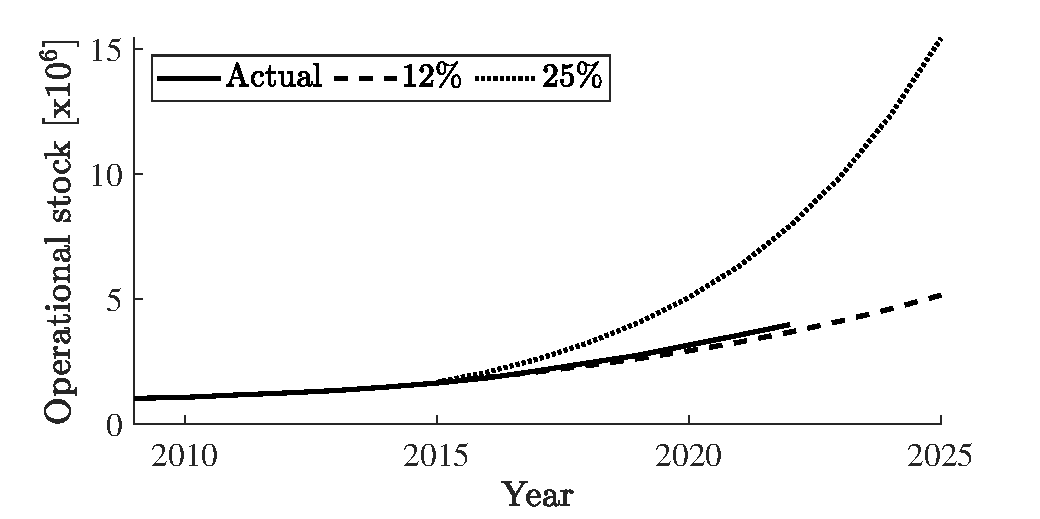
\includegraphics[width= 0.90\columnwidth]{fig/ir_units_projections.pdf} \label{fig:ir_stock}}
	\hfill
	\subfloat[]{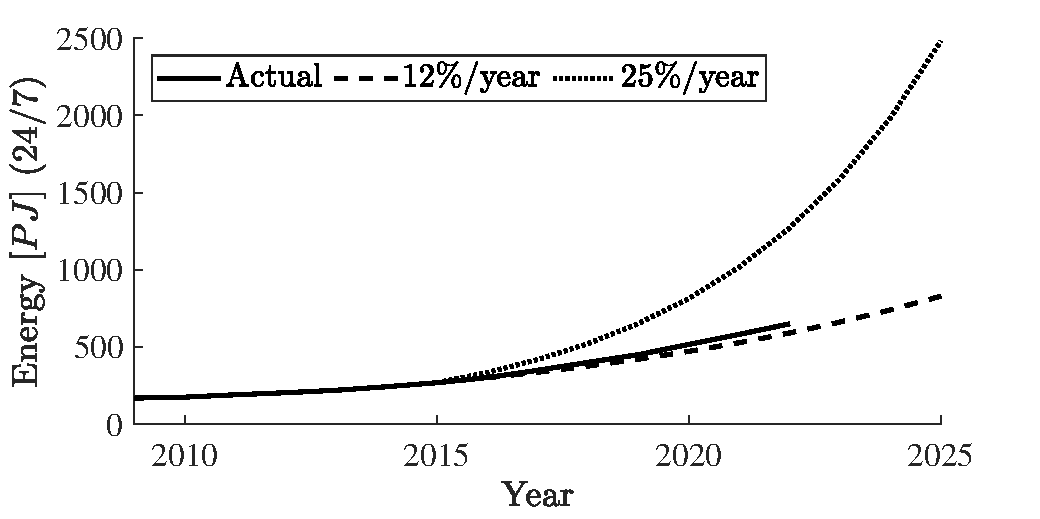
\includegraphics[width= 0.90\columnwidth]{fig/ir_energy_projections.pdf} \label{fig:ir_energy}}
	\hspace*{\fill}
	\\%[-2ex]
	\hspace*{\fill}
	\subfloat[]{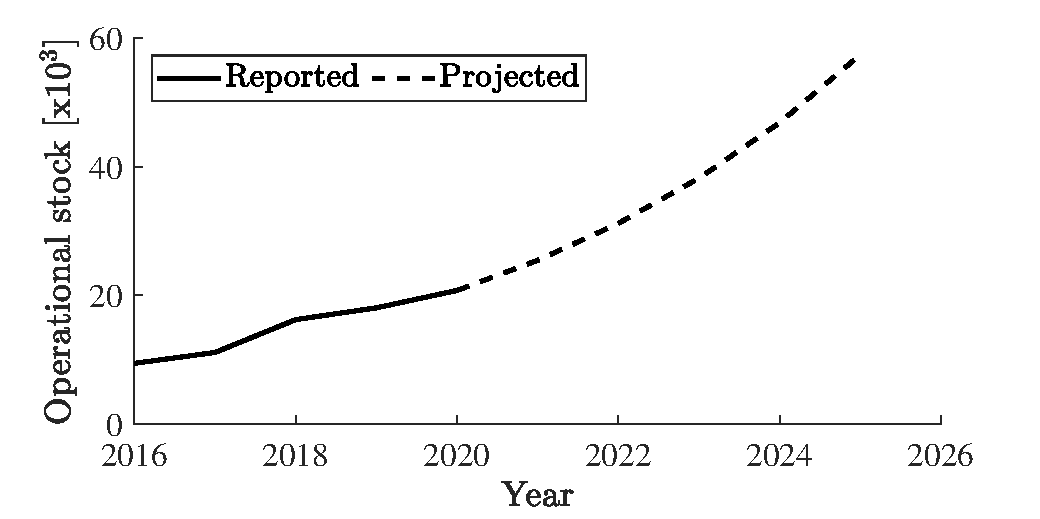
\includegraphics[width= 0.9\columnwidth]{fig/cb_units_projections.pdf}\label{fig:cobot_stock}}
	\hfill    
	\subfloat[]{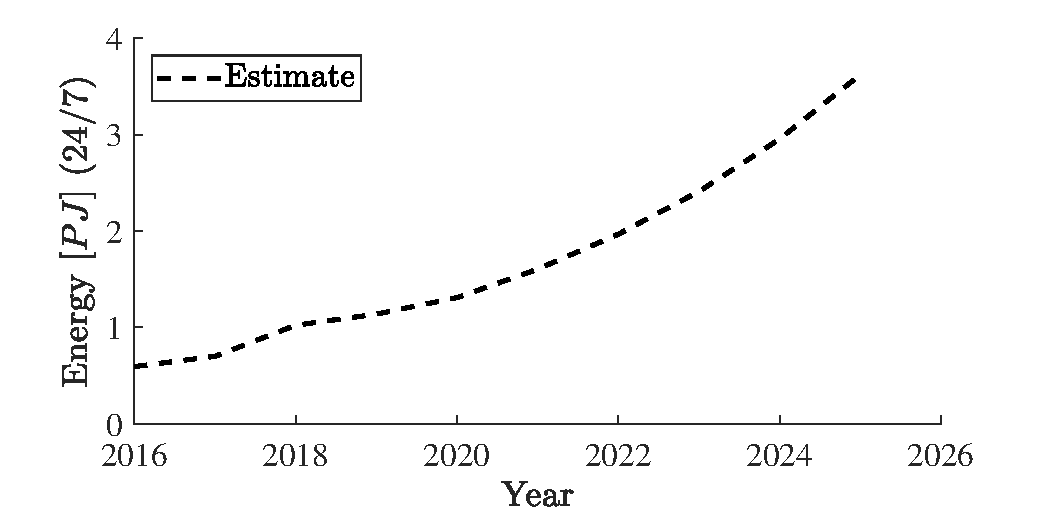
\includegraphics[width= 0.9\columnwidth]{fig/cb_energy_projections.pdf}\label{fig:cobot_energy}}
	\hspace*{\fill}    
	\caption[] {\label{fig:robot_forecasts} Forecasts for robot operational stock reported by the IFR and energy consumption estimates: \subref{fig:ir_stock} industrial robots install base forecast and \subref{fig:ir_energy} estimated worldwide energy consumption,  \subref{fig:cobot_stock} cobots install base forecast and their \subref{fig:cobot_energy} estimated worldwide energy consumption.}
\end{figure*}
%---
% SUBSECTION ========================================================================================
\subsection{\textbf{CHALLENGE 3} (C3). Energy for manufacturing}
Although not the focus of this work we briefly discuss this challenge for completeness and to motivate its study in future works. This last challenge expands the scope and considers the energetic cost pertaining to the manufacturing process of the EAI agents. It involves, firstly, the energy to procure the materials needed for the manufacturing of robots and the computation infrastructure. Secondly, the energy demanded by the manufacturing process itself. As the energy needed for material procurement and the manufacturing process is directly linked to the number of EAI agents being manufactured, it can be logically concluded that if their numbers increase exponentially, so will the energy consumed to produce them. Analysing this demand and devising strategies to handle it are at the center of this challenge. Although no clear solution is apparent, and since  meaningful energy savings in the procurement of the raw materials does not seem to be realistic possibility, we see in robot recycling a large potential strategy for energy savings. As a final thought, it is likely that in the future, the manufacturing of EAI agents will be conducted by other EAI agents (e.g. see Fig.~\ref{fig:franka_builds_franka}); thus connecting this challenge directly with the first two challenges.

%\textcolor{red}{The first two challenges addressed energy demand derived from the main composing elements of embodied AI. This last challenge deals with a broader perspective and considers the manufacturing of the hardware itself. Although not the focus of this work we briefly discuss this challenge for completeness and to motivate its study in future works. The production of EAI agents involves, firstly, energy to procure the materials (e.g. metal and plastic) needed for the manufacturing of robots and the computation infrastructure. Secondly, the energy necessary for the manufacturing process itself needs to be accounted for. Roughly, as the energy needed for material procurement an manufacturing process is directly linked to the number of robots being manufactured, and considering the exponentially increasing number of robots in service, a logical extrapolation is that this energy will also increase substantially. Analysing this demand and devising strategies to handle it are at the center of this challenge. However, to the best of our knowledge, there is a lack of studies that formally address the amount of energy needed to manufacture a robot. To provide a rough estimate of this demand, we leverage numbers from other well researched related areas and transfer them to the robot manufacturing context. In particular, we use records from the car manufacturing industry \cite{sullivan2010energy} and assume the \emph{technological density} of a robot and a car to be similar. As a result, we estimate that energy-wise, the demand to manufacture one ton of robots in analogous to manufacturing one ton one ton of cars. An average car with $\unit[1.5]{t}$ needs up to $\unit[34]{MJ}$ and up to $\unit[70]{t}$ \textcolor{red}{\textbf{[REF]}} of raw material. For example, \textcolor{red}{via direct scaling} one single KUKA 240 weighing $\unit[2]{t}$ \textcolor{red}{\textbf{[REF]}} is estimated to roughly need up to $\unit[45]{MJ}$ of energy and $\unit[90]{t}$ of raw materials. Simply multiplying this result by the numbers shown in Fig.~\ref{fig:ir_stock} gives already an idea of the magnitude of this challenge.  Although no clear solution is apparent, and since  meaningful energy savings in the procurement of the raw materials does not seem to be realistic possibility, we ponder that large potential energy savings would come from robot recycling. Nonetheless, this discussion is left for a latter occasion. As a final thought, it is likely that in the future, the manufacturing of embodied AI systems will be conducted by other embodied AI systems (eg. see Fig.~\ref{fig:franka_builds_franka}); thus connecting this with the first two challenges.}

%---
\begin{figure}[!t]
	\centering
	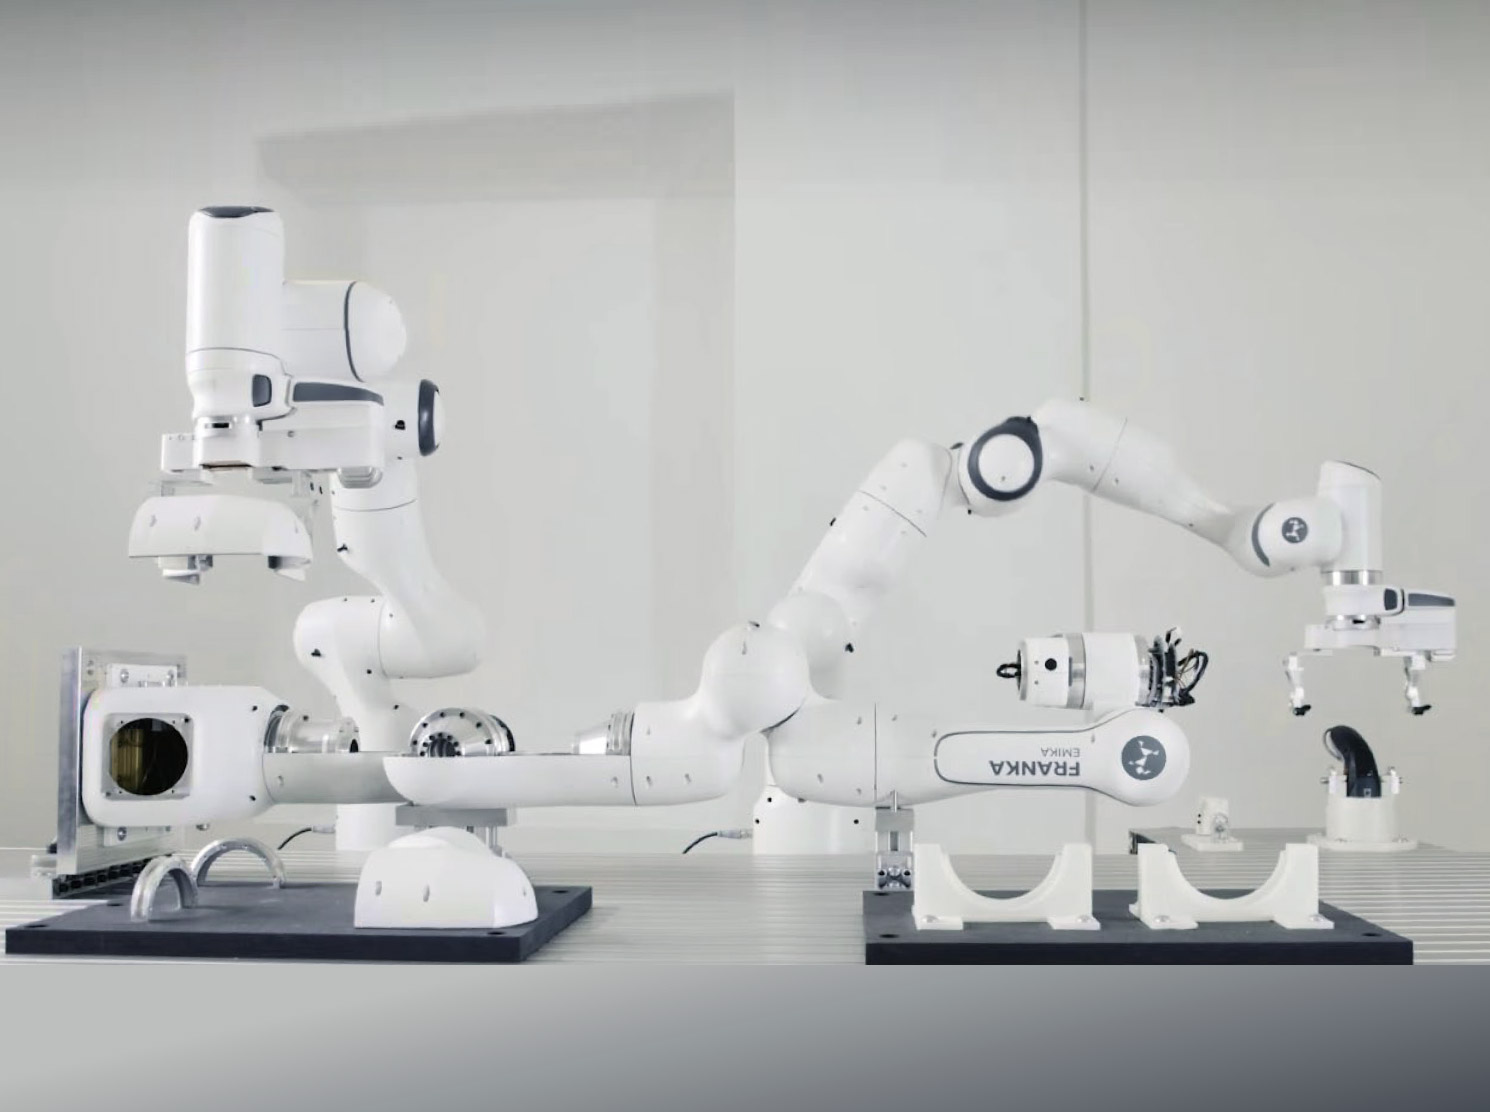
\includegraphics[width=0.75\columnwidth]{fig/franka_builds_franka.jpg}
	\caption{Robots manufacturing more robots}
	\label{fig:franka_builds_franka}
\end{figure}
% ---
% SUBSECTION ========================================================================================
\subsection{Potential research directions}
To identify areas of opportunity given the previously discussed challenges we first need to consider a crucial fact: for any given task, there is a physical limit to the energy that can be saved. To understand this consider the following, let $\tau$ be a desired skill for an EAI agent; for instance, pick-and-place. Additionally, assume that the optimal trajectory $p$ to move the object from origin to destination is known. Then, the properties of the to-be-moved object and the path $p$ fully determine the minimum energy $E^*_{\tau}$ required to execute skill $\tau$. This means that an embodied AI agent attempting to execute $\tau$ will consume at least this amount of energy. In reality, however, the total energy required for learning and executing a skill comprises the sum of $E^*_{\tau}$ plus the accompanying computational $E_{CCE}$, body-related $E_{BEE}$ and motion and interaction $E_{MIE}$ energy requirements during learning and execution; i.e.
% ---
\begin{equation}
     E_{\tau} =  E^*_{\tau} +  E_{CCE} +  E_{BEE} +  E_{MIE}.
\end{equation}
% ---
Fig.~\ref{fig:challengesConnected} depicts the potential connections that exist between the grand challenges and the energy expenditure categories that are relevant for each of them. Related to \textbf{challenge 1} and $E_{CCE}$, one direction that the embodied AI research community should focus is on developing energy-aware algorithms. Either by focusing on more data-efficient approaches, embedding relevant prior knowledge in the architecture, or knowledge sharing capabilities. The last, in particular, would be an ideal candidate solution due to its raw potential. An algorithm capable of sharing knowledge would allow for high efficiency in multi-skill learning and, associated with a cloud-connected library of skills, accelerate new skill learning on every EAI agent connected to it. This approach would, over time, convert the processing requirement of the data centers into mostly database storage and query, which is much less energy demanding. Additionally, better computational algorithms could be defined aided running in more efficient processing and supported by more efficient communication mechanisms. As for \textbf{challenge 2}, most of the problem is attributed to the rapid growth in the numbers of active robots that will power future manufacturing industry but their potentially energy inefficient design and/or wasted capabilities should not be disregarded; thus it is related to $E_{BEE}$ and $E_{MIE}$. Since there is no actual control over the eventual number of robots, new designs with light weight materials and elastic elements that foster the efficient use of the available energy to perform a skill should be pursued. These new mechatronic designs should, in turn, be exploited by embodied AI algorithms researched in \textbf{challenge 1} to find yet better solutions to learn and execute skills. Finally, \textbf{challenge 3}, is highly intertwined with other two challenges and, thus, is linked to three types of energy $E_{CCE}$, $E_{BEE}$ and $E_{MIE}$. This means that improvements in the challenge 1 and 2 will yield improvements in challenge 3. Yet, a vital direction to save energy in manufacturing is recycling. A competent recycling process is coupled with the manufacturing where robots that end their service life can be harvested for materials and parts, a zero waste policy could be implemented. 
% ---
\begin{figure}[!t]
	\centering
	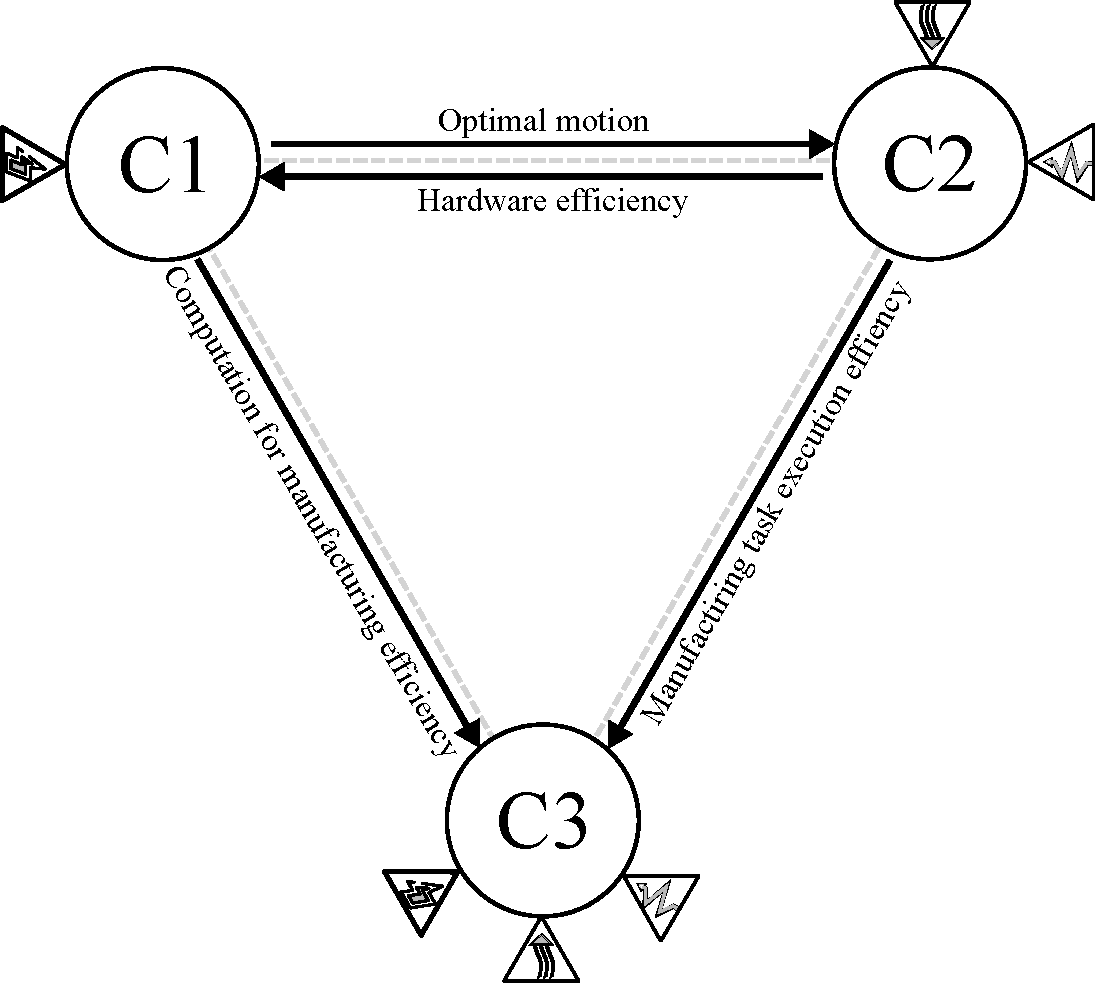
\includegraphics[width=0.9\columnwidth]{fig/grand_challenges_connections_v2.pdf}
	\caption{Interconnection of the different challenges.}
	\label{fig:challengesConnected}
\end{figure}
% ---

% ===================================================================================================
%                                                 |                                                 |
%                                                 |                                                 |
% -------------------------------------------- SECTION ---------------------------------------------|
%                                                 |                                                 |
%                                                 |                                                 |
% ===================================================================================================
% ===================================================================================================
%                                                 |                                                 |
%                                                 |                                                 |
% -------------------------------------------- SECTION ---------------------------------------------|
%                                                 |                                                 |
%                                                 |                                                 |
% ===================================================================================================
\section{Learning paradigms for embodied AI (EAI) agents}\label{sec:learning_paradigms}
In this section we model the scaling of energy and time demand that results from the use of a team of robots learning a universe $\mathcal{S}=\left\lbrace s_1,s_2,\ldots s_j,\ldots, s_{N_\mathcal{S}}\right\rbrace$ of skills, with $|\mathcal{S}| = N_\mathcal{S}$.

% ===================================================================================================
\subsection{Energy and time demand for learning skills}
%---
\begin{tcolorbox}
	\begin{definition}\label{definition:complexity}
		The complexity $c_j$ of a skill $ s_j $  is the number of trial episodes $n$ needed to successfully learn the skill; i.e., all actions and states visited until a stopping criterion is reached. 
	\end{definition}
\end{tcolorbox}
% ---

%To simplify the analysis we make the conservative assumption that the power $P_0$ required by any given robot to learn of a skill is constant. Furthermore,% ---
To simplify the analysis consider the following conservative assumption
% ---
\begin{tcolorbox}
	\begin{assumption}\label{assumption:time}
		Given a large number of robots performing a large number of skills, the average power $P_0$ required by any given robot during learning and the average time $\Delta t$ allocated to the execution of every trial episode $n$ are constant, see Fig.~\ref{fig:power_per_episode}.
	\end{assumption}
\end{tcolorbox}
% ---
% ---------------------------------------------------------------------------------------------------
\subsubsection{\textbf{Episode, skill, and skill set energy requirements}}
% ---
\begin{figure}[!t]
	\centering
	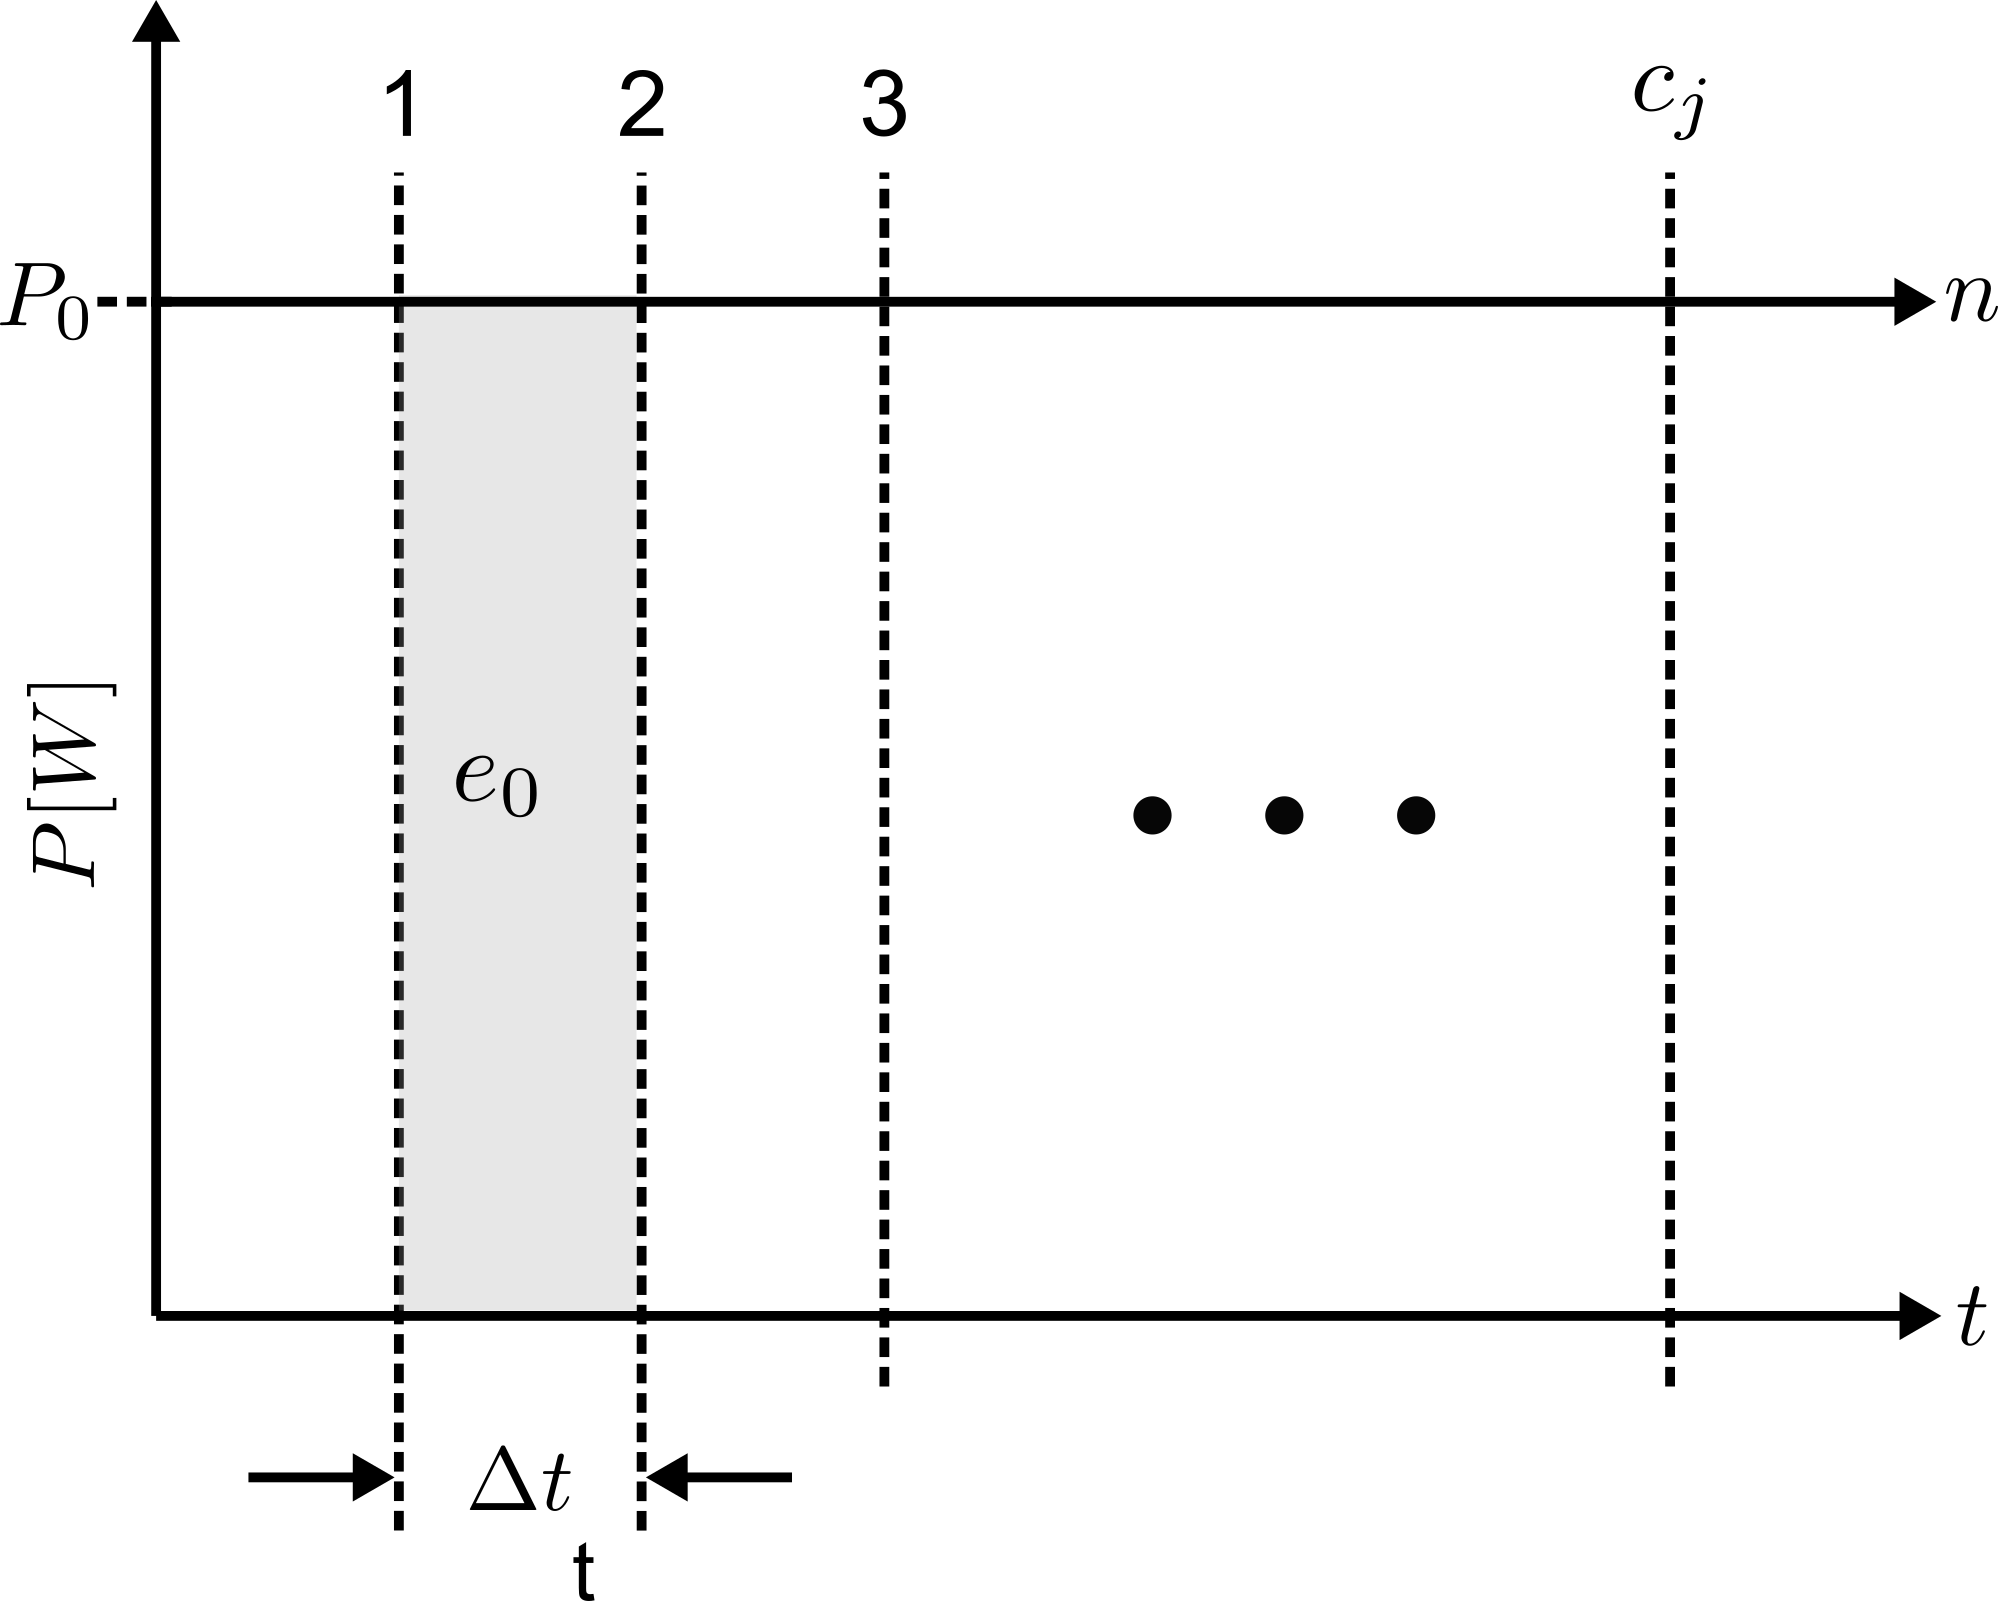
\includegraphics[width=0.95\columnwidth]{fig/power_per_episode.png}
	\caption{Power consumption per episode.}
	\label{fig:power_per_episode}
\end{figure}
% ---
Under Asm.~\ref{assumption:time}, the energy consumption of the $n$-th episode $e_j(n)$ is the constant product
% ---
\begin{equation}\label{eq:energy_per_episode}
    e_j(n) = \underbrace{P_0 \Delta t}_{\text{constant}} = e_0.
\end{equation}
% ---
Consequently, the energy consumed by a robot learning a skill $ s_j $ is directly proportional to the skill complexity $c_j$; i.e.
% ---
\begin{equation}\label{eq:energy_per_skill}
    E_j =\sum_{n=1}^{c_j} e_j(n) = e_0c_j.
\end{equation}
% ---
The energy spent on learning $\mathcal{S}$ under the absence of knowledge transfer is
% ---
\begin{equation}\label{eq:total_energy}
	E_{\mathcal{S}} = \sum_{j=1}^{{N_{\mathcal{S}}}} E_j = e_0 \sum_{j=1}^{{N_{\mathcal{S}}}} c_j%N_{\mathcal{T}} \cdot e_0 \cdot c_j 
\end{equation}
% ---
% ---------------------------------------------------------------------------------------------------
\subsubsection{\textbf{Time requirement}}
Similarly, the total learning time $T_{\mathcal{S}}$ for a simple agent is
% ---
\begin{equation}\label{eq:total_energy}
	T_{\mathcal{S}} = \Delta t \sum_{j=1}^{{N_{\mathcal{S}}}} c_j.
\end{equation}
% ---
As a consequence of Asm.~\ref{assumption:time} and \eqref{eq:energy_per_skill}, in the remaining of this section analyzing the complexity of a skill or set of skills is equivalent to analyzing the energy demand of its learning process.
% ===================================================================================================

\subsection{Similarity and knowledge}
%---
\begin{tcolorbox}
	\begin{assumption}\label{assumption:skill_clustering} If the similarity among a set of skills is significant, the exchange of acquired knowledge from these skills expedites the overall learning process.
		\end{assumption}
\end{tcolorbox}
% ---
Let $\mathcal{Z}_k \subset \mathcal{S}$ be a subset of $N_{\mathcal{Z}_k}$ skills that share high similarity; i.e. a \emph{cluster} of similar skills, see Fig.~\ref{fig:skill_similarity}. Furthermore, consider a second set $\mathcal{\zeta}_k \subset \mathcal{Z}_k$ that denotes already learned skills from $\mathcal{Z}_k$. Asm.~\ref{assumption:skill_clustering} implies that the $j$-th skill in the $k$-th cluster $s_{j,k} \in \mathcal{Z}_k$ can always benefit from the knowledge contained in $\mathcal{\zeta}_k$. This implies that the more skills enter $\mathcal{\zeta}_k$, the less knowledge about $ s_{j,k} $ will remain to be learned.
% ---
\begin{figure}[!t]
	\centering
	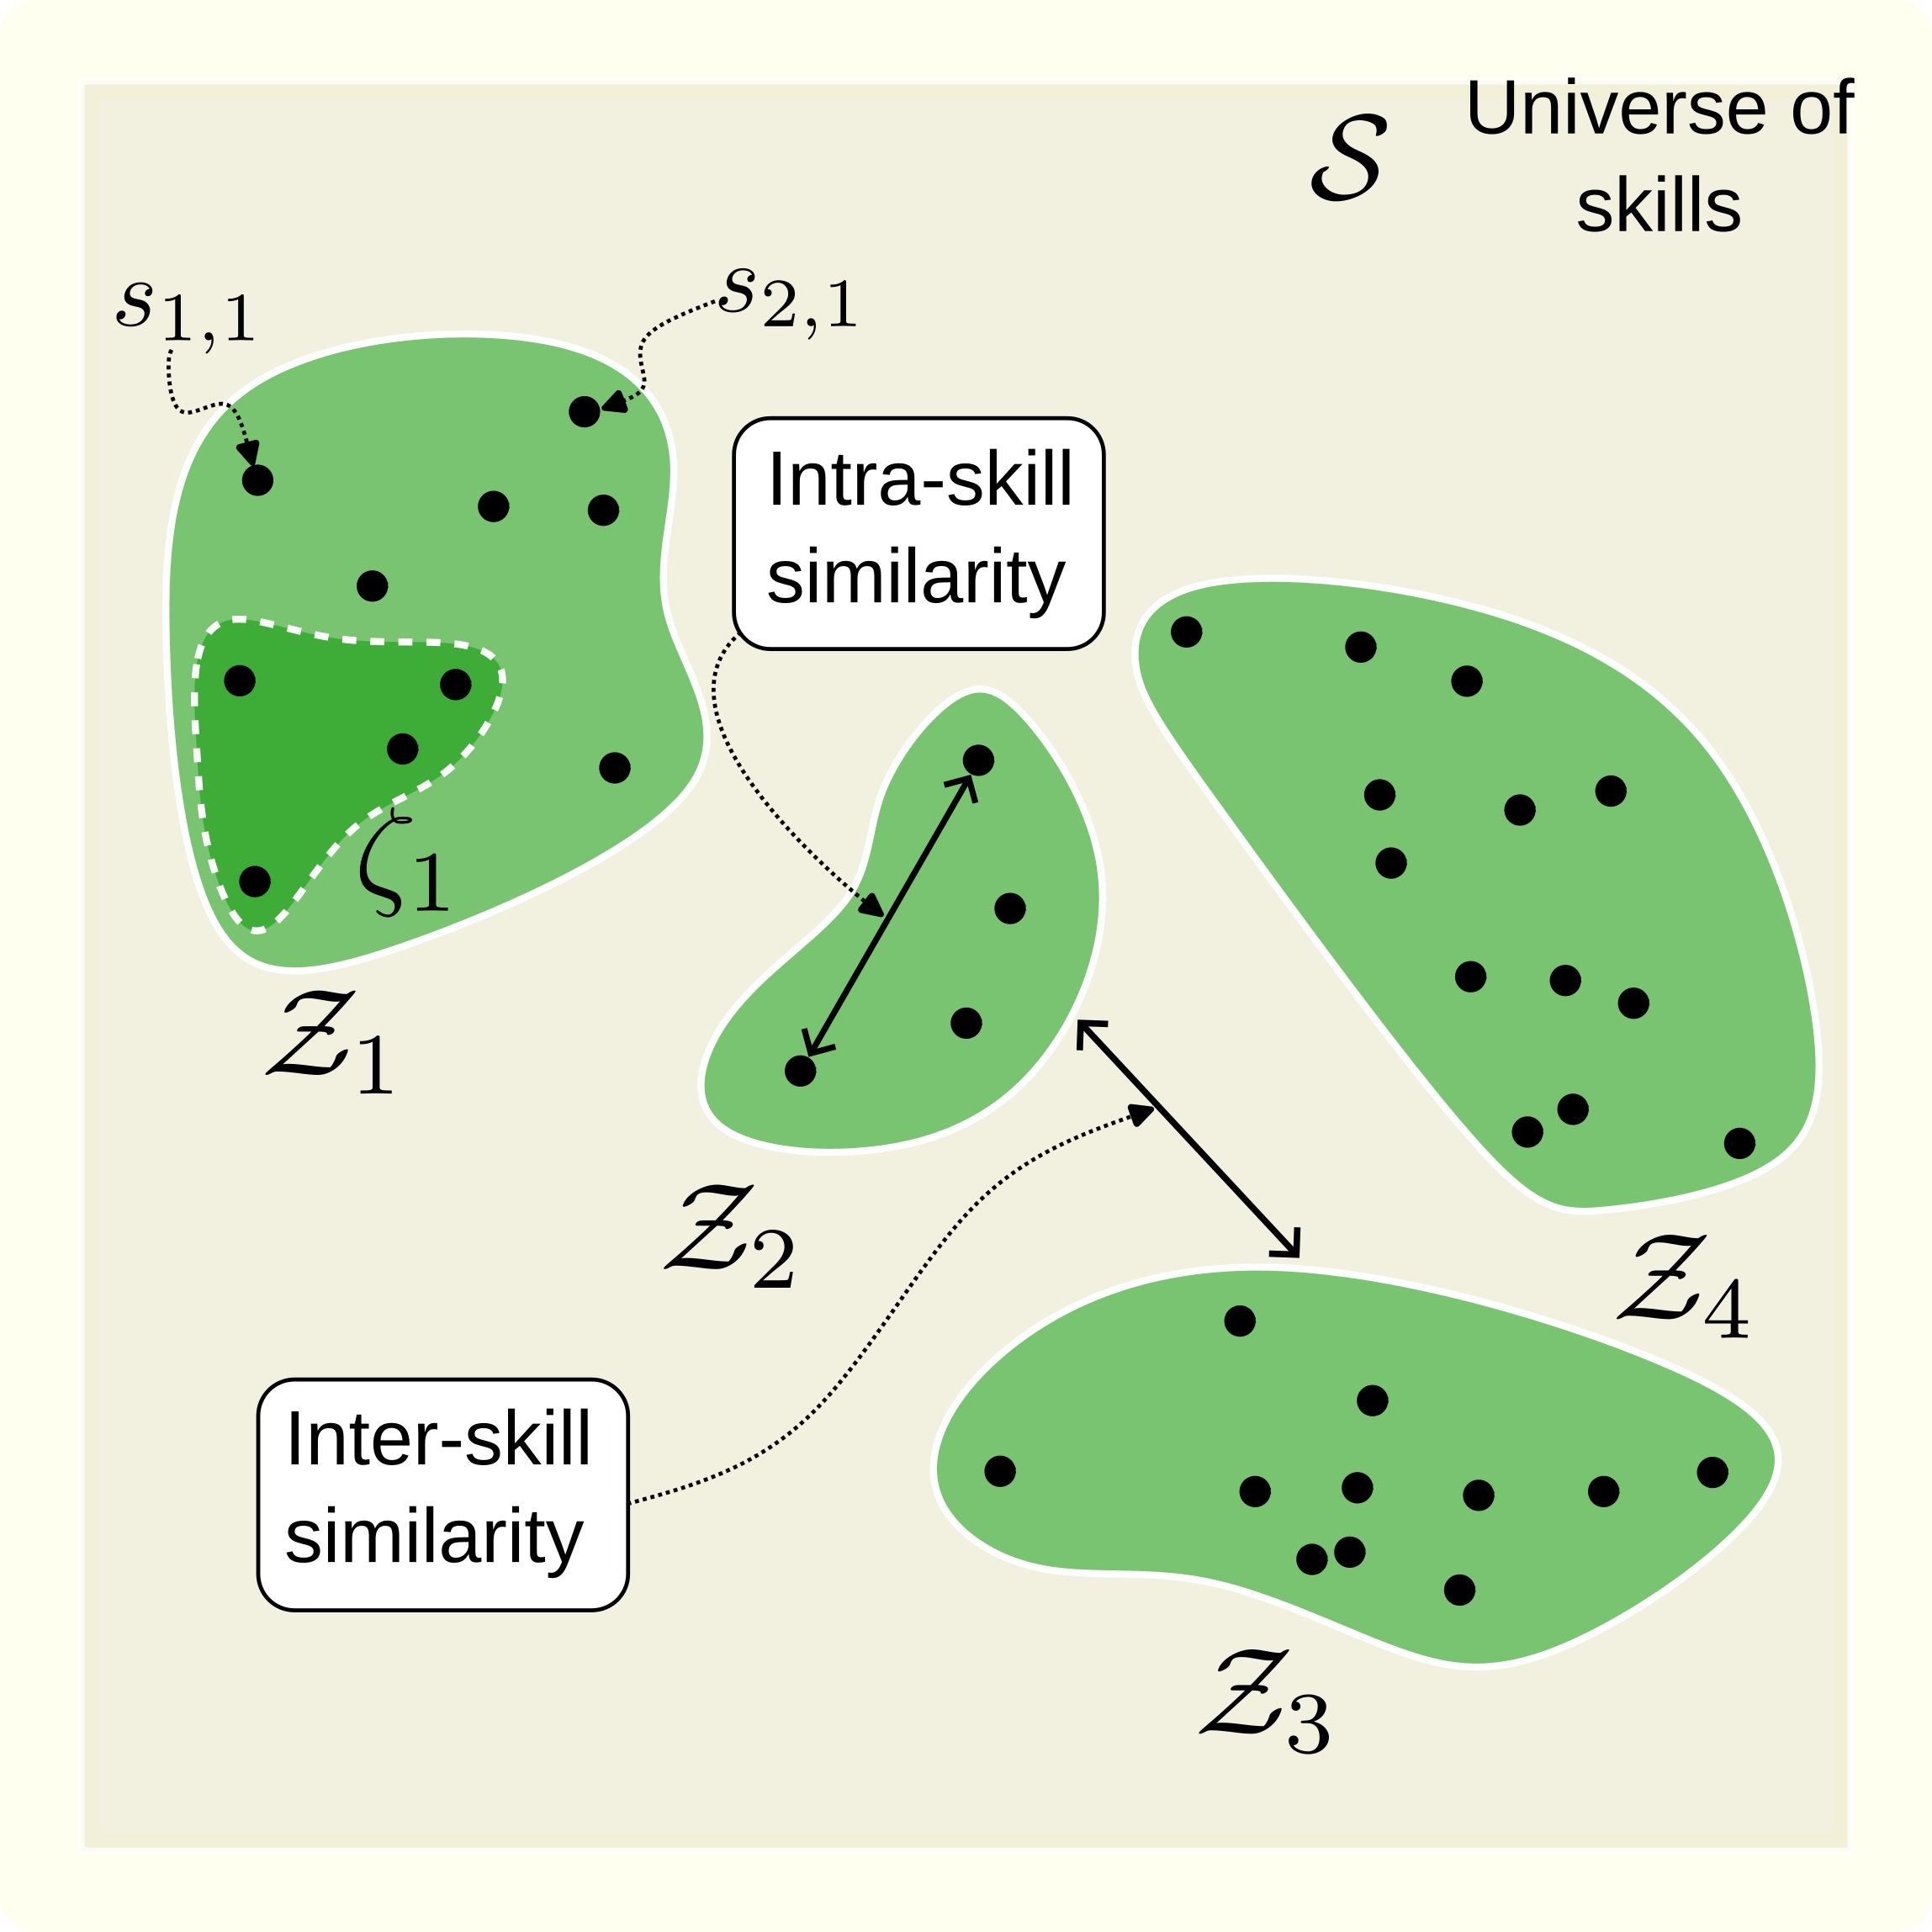
\includegraphics[width=0.95\columnwidth]{fig/skill_similarity.png}
	\caption{Similar skills in $\mathcal{S}$ can be grouped into clusters $\mathcal{Z}_k$.}
	\label{fig:skill_similarity}
\end{figure}
% ---
Now, we introduce a function $\bar{\sigma}_{j,k}\left(n\right)\in [0,1]$ that expresses the knowledge about a skill $s_{j,k} \in \mathcal{Z}_k\textbackslash \mathcal{\zeta}_k$ that \textbf{is not} contained in $\mathcal{\zeta}_k$. The function $\bar{\sigma}_{j,k}(\cdot)$ satisfies:
% ---
%\begin{itemize}
%	\item $\bar{\sigma}_{j,k}\left(n\right) = 1$, if $\mathcal{\zeta}_k=\emptyset$ or if it does not contain knowledge about the skill $s_{j,k}$
%	\item $\bar{\sigma}_{j,k}\left(n\right) = 0$, if \emph{all} the knowledge about skill $s_{j,k}$ is contained in $\mathcal{\zeta}_k$
%\end{itemize} 
% ---
\begin{equation}\label{eq:sigma_bar_conditions}
	\bar{\sigma}_{j,k}\left(n\right) = 
	\begin{cases}
		1 & \text{$\mathcal{\zeta}_k=\emptyset$}\\
		0 &\text{$\mathcal{\zeta}_k$ has \emph{all} knowledge of $s_{j,k}$}
	\end{cases}
\end{equation}
Conceptually, $\bar{\sigma}_ {j,k}\left(\cdot\right)$ is the fraction of knowledge from ${\mathcal{Z}_k}$ that remains to be learned.

% ---------------------------------------------------------------------------------------------------
\subsubsection{\textbf{Leveraging the acquired knowledge}}
To evaluate the effect of knowledge exchange during learning we introduce an upper bound called the skill \textit{fundamental complexity}.
% ---
\begin{tcolorbox}
	\begin{definition}\label{assumption:fundamental_complexity}
		The fundamental complexity $c_0$ describes the maximum number of trial episodes required to learn \emph{any} skill.
	\end{definition}
\end{tcolorbox}
% ---
If, in learning a skill $ s_{j,k} $, a robot uses the knowledge contained in $\mathcal{\zeta}_k$; then, two effects take place:
% ---
\begin{enumerate}
	\item There is less remaining knowledge, reflected in the initial value; i.e. $\bar{\sigma}_{j,k}(0) < 1$
	\item The knowledge acquisition rate increases
\end{enumerate}
% ---
%associated complexity $ c_{j,k} $ is necessarily smaller than the fundamental complexity $c_{0}$; i.e. $c_{j,k} < c_0~\forall j>1$.
This implies that the remaining knowledge scales down as a function of the number of learned skills $N_{\zeta_k}=|\mathcal{\zeta}_k|$. As a consequence, the complexity $c_{j,k}$ of said skill is smaller than the fundamental complexity $c_0$.%, as exemplified in Fig.~\ref{fig:complexity_per_cardinality}. 

The effects of knowledge exchange lead us to introduce another assumption.
% ---
\begin{tcolorbox}
	\begin{assumption}\label{assumption:exponential_decrease} The remaining knowledge function $\bar{\sigma}_{j,k}(\cdot)$ has a monotonically decreasing behavior.
	\end{assumption}
\end{tcolorbox} 
% ---
\noindent

% ---
%\begin{subequations}\label{eq:simple_knowledge_dynamics}
%	\begin{alignat}{2}
%		\dot{\bar{\sigma}}_{j,k}\left(n\right) &= -\alpha r f\left(N_{\zeta_k}\right) \bar{\sigma}_{j,k}\left(n\right)\\
%		\bar{\sigma}_{j,k}(0) &= g\left(N_{\zeta_k}\right)
%	\end{alignat}
%\end{subequations}
An idealization of the behavior satisfying Asm.~\ref{assumption:exponential_decrease} and \eqref{eq:sigma_bar_conditions} can be modeled via a differential equation.
\begin{tcolorbox}
	\begin{definition}\label{assumption:ode_model}
		The remaining knowledge function $\bar{\sigma}_{j,k}$ is modeled as the first order linear differential equation
		\begin{subequations}\label{eq:simple_knowledge_dynamics}
			\begin{alignat}{2}
				\dot{\bar{\sigma}}_{j,k}\left(n\right) &= -f_{j,k} \left(N_{\zeta_k} \right) \bar{\sigma}_{j,k}\left(n\right),\\
				\bar{\sigma}_{j,k}(0) &= g_{j,k} \left(N_{\zeta_k}\right).
			\end{alignat}
		\end{subequations}
	\end{definition}
\end{tcolorbox} 
% ---
Eq.~\eqref{eq:simple_knowledge_dynamics} depends on the trial episodes $n$ and is parameterized by the number of already learned skills $N_{\zeta_k}$. Its solution
% ---
\begin{equation}\label{eq:knowledge_exponential_form}
	\boxed{\bar{\sigma}_{j,k}(n) = g_{j,k}\left(N_{\zeta_k}\right) e ^{-f_{j,k}\left(N_{\zeta_k}\right) n} \in (0,1]},
\end{equation}
% ---
exhibits the desired, shown in Fig.~\ref{fig:knowledge_idealization}. The function $f_{j,k}\left(N_{\zeta_k}, r\right)$ models one of the effects resulting from the exploitation of the knowledge available in $\zeta_k$, namely, the increase of the learning rate. The second effect, i.e. the reduction in the initial remaining knowledge $\bar{\sigma}_{j,k}(0)$ is controlled by the term $g_{j,k}\left(N_{\zeta_k}\right)$, which is also dependent on the number of learned skills. The learning threshold $\epsilon$ indicates when the remaining knowledge is negligible and $s_{j,k}$ is considered as learned.
% ---
\begin{figure}[!t]
	\centering
	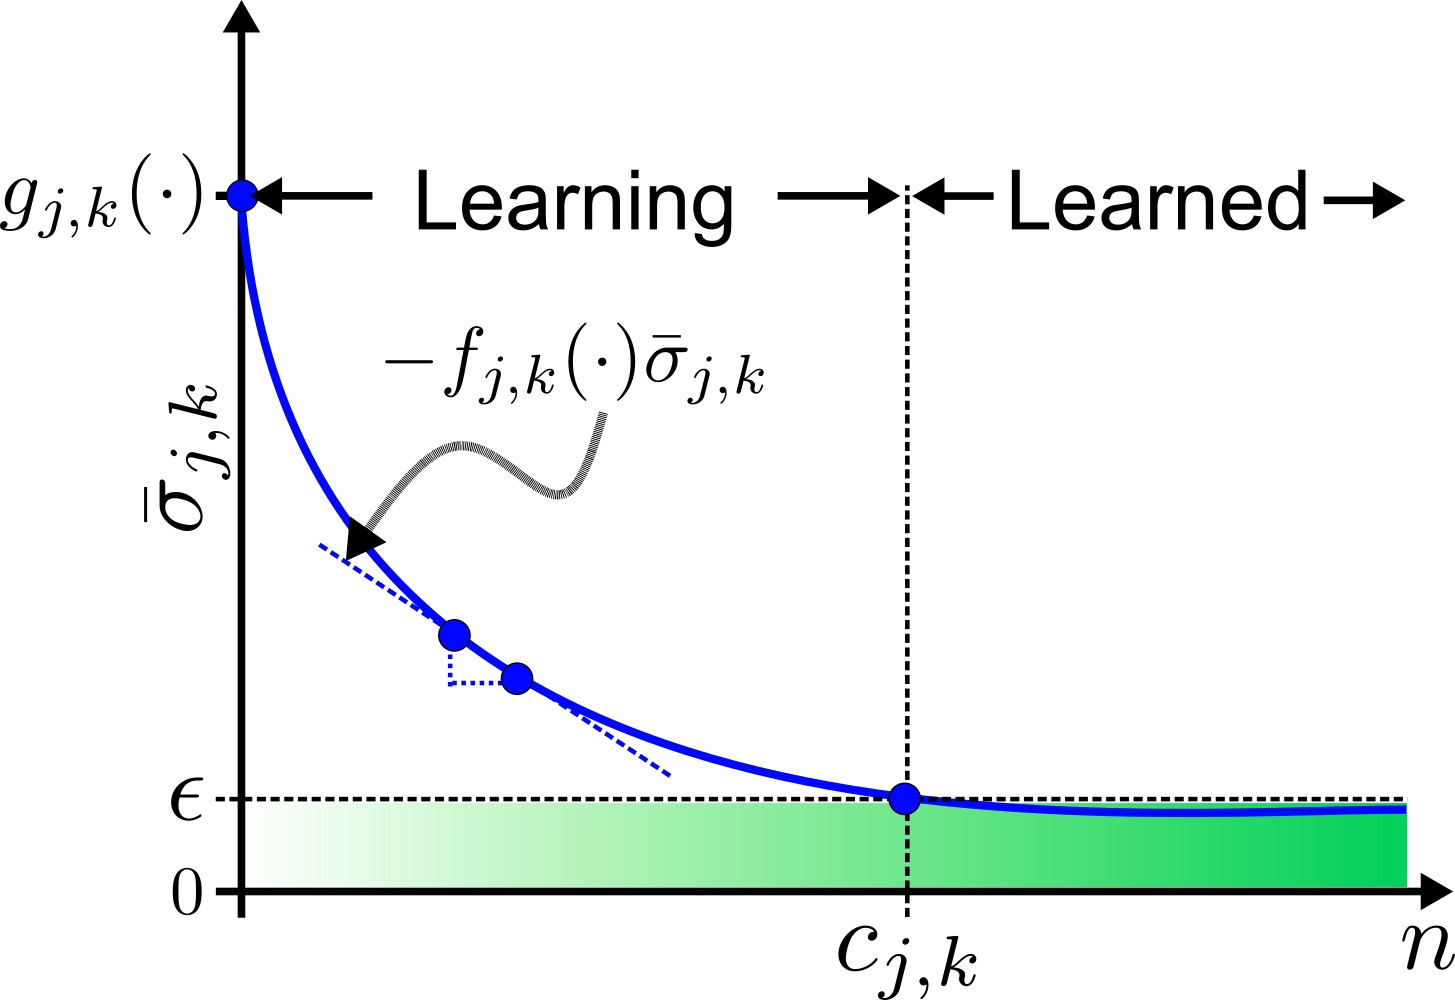
\includegraphics[width=0.95\columnwidth]{fig/knowledge_idealization.png}
	\caption{Remaining knowledge to learn a new skill $s_{j,k}$.}
	\label{fig:knowledge_idealization}
\end{figure}
% ---
% ===================================================================================================
\subsection{Knowledge sharing and transfer under different learning paradigms}
%The following assumptions are analogous to average behavior and imply that a suitable scaling strategy is available and executed.
%Before tacking the different learning schemes let us define the idealized reference system in which a large number of robots coexists learning a large number of skills.

For the upcoming analysis we consider an idealized reference system in which a large number of robots coexist learning a large number of skills. Such system exhibits
% ---
\begin{tcolorbox}
	\begin{assumption}\label{assumption:average_behavior}
		An average behavior that results from comparable EAI agents learning and executing the skills in $\mathcal{S}$ ordered and segregated according to their similarity.
	\end{assumption}
\end{tcolorbox}
%---
Each of the EAI agents in the system
\begin{tcolorbox}
	\begin{assumption}\label{assumption:agent_similarity}
		Has the same capabilities with highly similar BEE and MIE expenditures.
	\end{assumption}
\end{tcolorbox}
%---
The large number of skills in $\mathcal{S}$ implies that
% ---
\begin{tcolorbox}
	\begin{assumption}\label{assumption:cluster_size}
		Every cluster $\mathcal{Z}_{k}$ contains the same number $N_{\mathcal{Z}} $ of skills.
	\end{assumption}
\end{tcolorbox}
% ---
By virtue of the optimal ordering of the skills and the balanced size of the clusters,
% ---
\begin{tcolorbox}
	\begin{assumption}\label{assumption:cluster_transferability}
		The knowledge transferability between in-cluster skills ---modeled by \eqref{eq:f_function_incremental} and \eqref{eq:g_function_incremental}--- is assumed to be equal; as is transferability between clusters, see \eqref{eq:f_function_transfer} and \eqref{eq:g_function_transfer}.
	\end{assumption}
\end{tcolorbox}
% ---
Finally, the different learning paradigms that exploit the collected knowledge by the EAI agents rely on the fact that
% ---
\begin{tcolorbox}
	\begin{assumption}\label{assumption:enabling_agorithms}
	There are advanced control and machine learning algorithms designed to inherently use this knowledge.
	\end{assumption}
\end{tcolorbox}

% ---------------------------------------------------------------------------------------------------
\subsubsection{\textbf{Isolated Learning (IsL)}} A robot learns each skill in $\mathcal{Z}_k$ one after another from the ground up, disregarding the accumulating knowledge from already learned skills. In such a case the rate of convergence and the initial remaining knowledge for all skills are given by
% ---		
\begin{subequations}\label{eq:fg_isolated}
	\begin{alignat}{2}
		f_{j,k}\left(\cdot \right) &=  -\alpha \\
		g_{j,k}\left(\cdot \right) &= 1,
	\end{alignat}
\end{subequations}
% ---
where $ \alpha>0$ models the rate at which a robot in isolation learns any given skill. Relying on Asm.~\ref{assumption:agent_similarity} we can assign a value to $\alpha$ by using the fundamental complexity $c_0$ as follows
% ---
\begin{equation}\label{eq:isolated_learning_rate}
	\alpha = -\frac{1}{c_0}\text{log}(\epsilon).
\end{equation}
% ---
Since in isolated learning $c^{(IsL)}_{j,k} = c_0$, the trial episodes required by one single robot to learn the skills in the cluster $\mathcal{Z}_k$ is given by
% ---
\begin{align}
	\begin{split}
		C^{(IsL)}_{k} &= \sum_{j=1}^{N_{\mathcal{Z}}} c^{(IsL)}_{j,k}= N_{\mathcal{Z}}  \cancelto{c_{0}}{c^{(IsL)}_{j,k}} = N_{\mathcal{Z}} c_0
	\end{split}
\end{align}
%-- 
Similarly, the total trial episodes to learn the universe of skills is simply
% ---
\begin{equation}
	C^{(IsL)}_{\mathcal{S}} = N_\mathcal{K} N_{\mathcal{Z}} c_0.
\end{equation}
% ---
\paragraph*{Multi agent case}
Suppose that a batch of $m$ robots is used to learn the same number of skills in parallel in a given cluster $\mathcal{Z}_k$. Such a strategy only distributes equally the total number of episodes by the number of available robots; i.e.
% ---
\begin{equation}
	^{\lvert \lvert}C^{(IsL)}_k=  \overbrace{\frac{1}{m}C^{(IsL)}_k}^{\text{episodes per robot}}.
\end{equation}
% ---




%The energy required by one single robot to learn the skills in the cluster $\mathcal{Z}_k$ is given by
%% ---
% \begin{align}
%     \begin{split}
%       E^{(Iso)}_{\mathcal{Z}_k} &= \sum_{j=1}^{N_{\mathcal{Z}}} E^{(Iso)}_j= N_{\mathcal{Z}_k}  e_{0} \cancelto{c_{0}}{c_{j,k}} = N_{\mathcal{Z}} e_{0}  c_0
%     \end{split}
% \end{align}
%%-- 
%If $\mathcal{S}$ is divided into $\left\lbrace \mathcal{Z}_k \right\rbrace^{N_\mathcal{K}}_{k=1} $ clusters, the total energy to learn the universe of skills is simply
%% ---
%\begin{equation}
%	E^{(Iso)}_{\mathcal{S}} = N_\mathcal{K} N_{\mathcal{Z}} e_{0}  c_0.
%\end{equation}
%% ---
%\paragraph*{Multi agent case}
%Notice that using a batch of $m$ robots to learn the same number of skills in parallel does not bring about any energy reductions since
%% ---
%\begin{equation}
%    ^{\lvert \lvert}E^{(Iso)}_\mathcal{S}= \underbrace{m}_{\text{robots}}\cdot \overbrace{\frac{1}{m}E^{(Iso)}_\mathcal{S}}^{\text{energy per robot}} = E^{(Iso)}_\mathcal{S}.
%\end{equation}
%% ---


%---
% \begin{figure}[!ht]
% 	\centering
% 	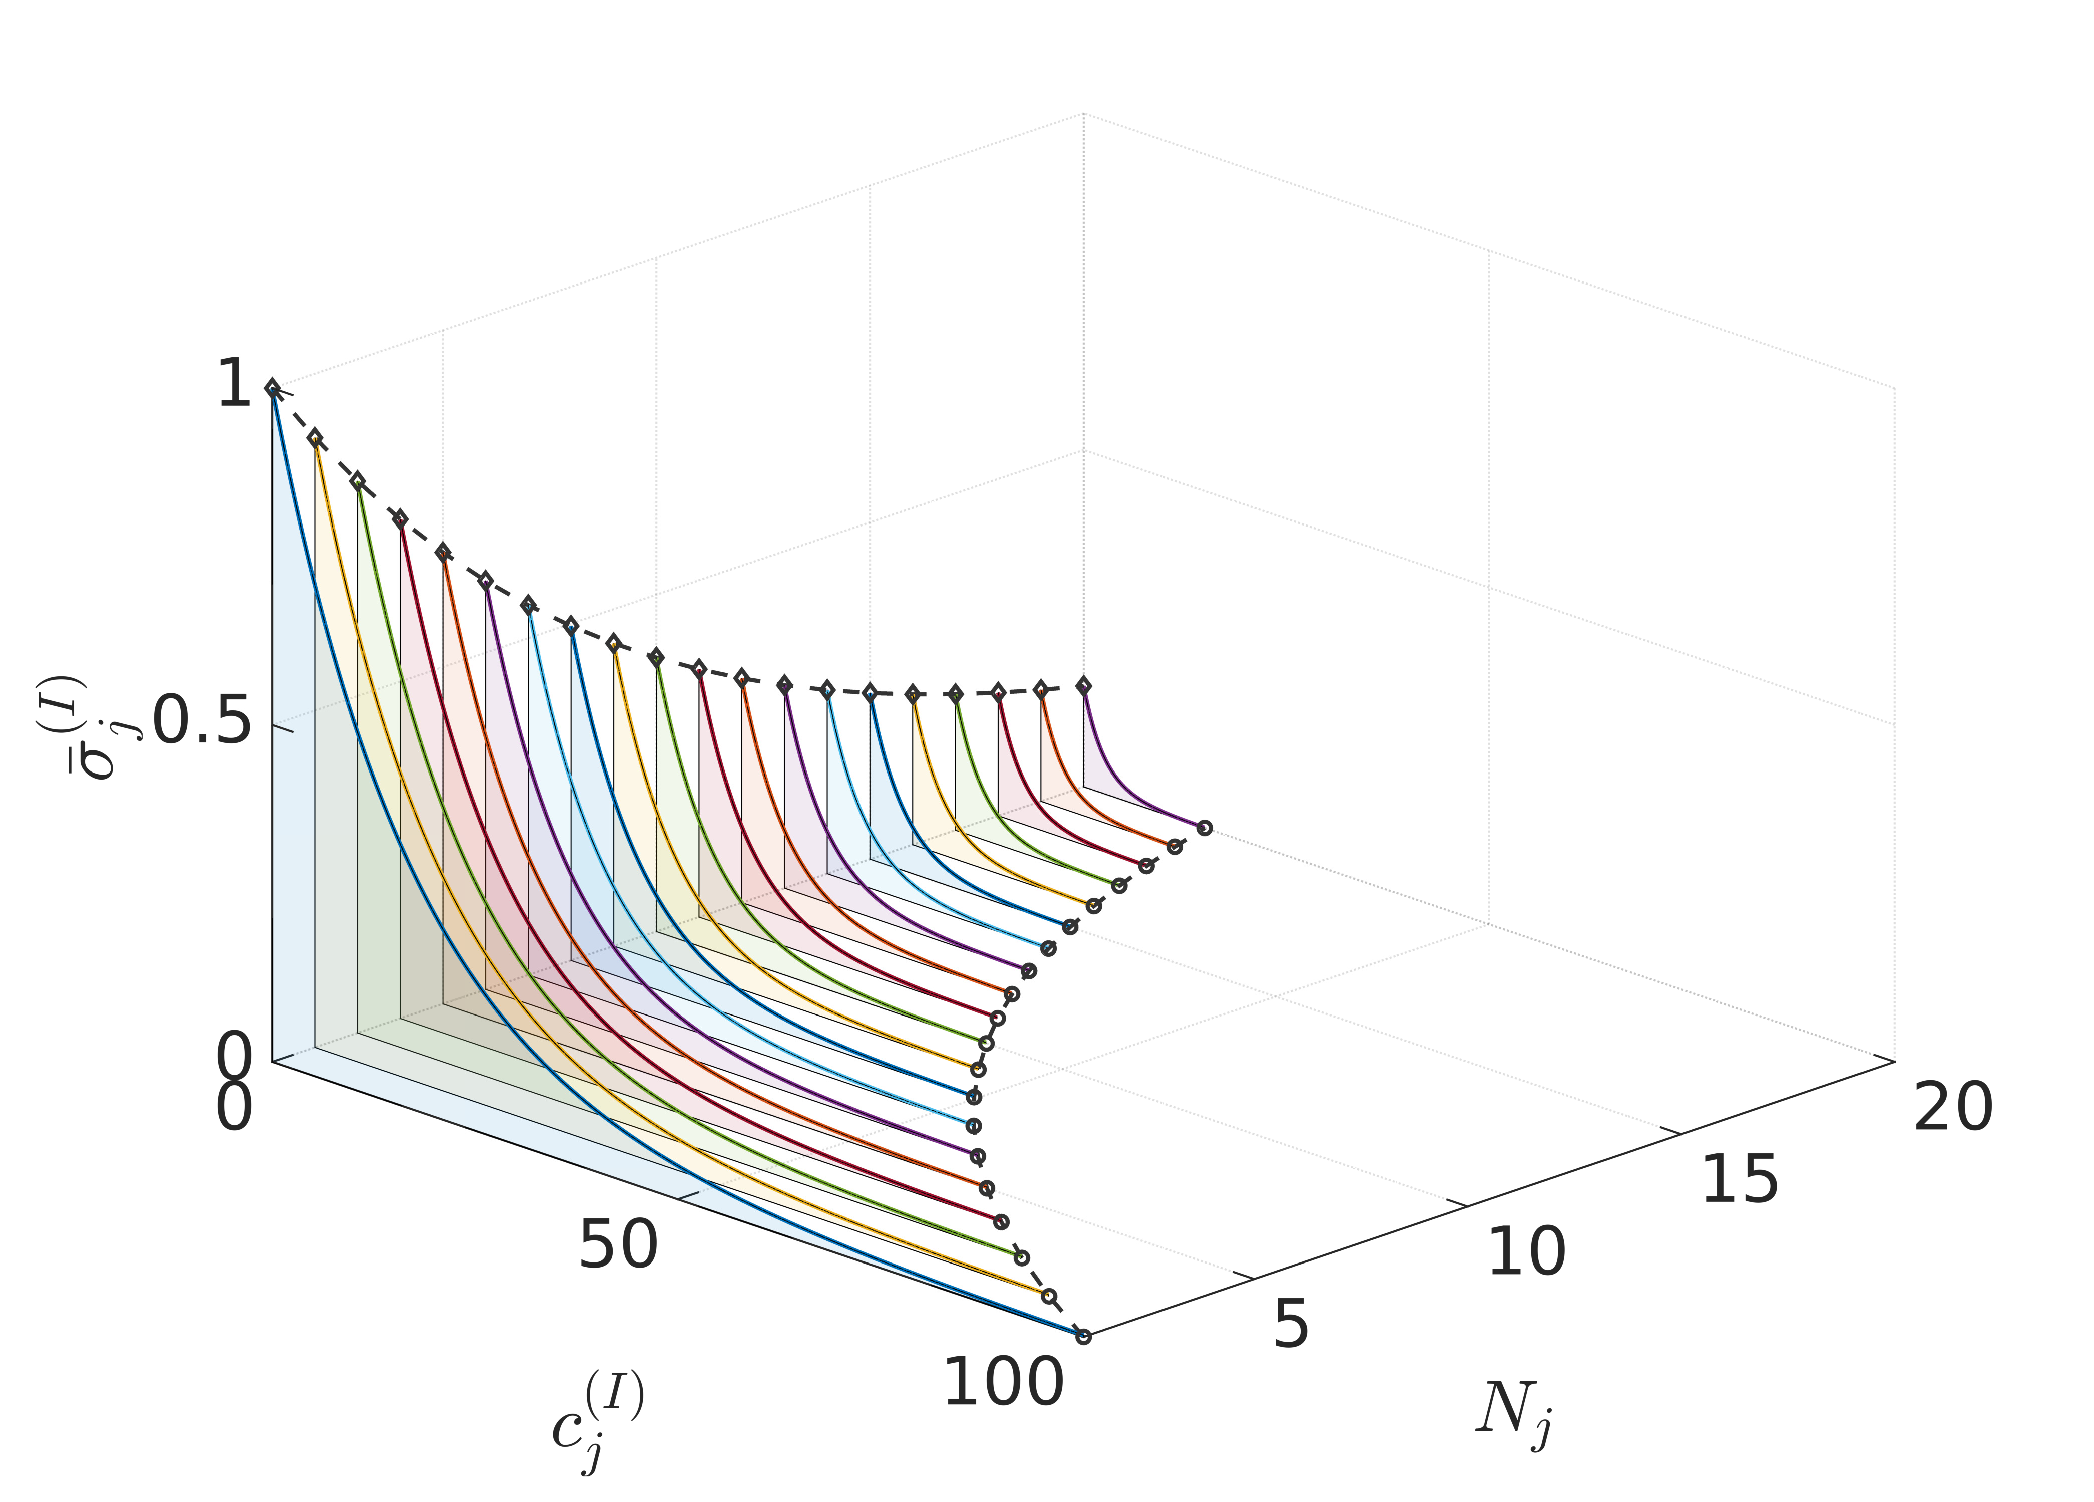
\includegraphics[width=0.99\columnwidth]{tex/fig/single_incremental_knowledge.pdf}
% 	\caption{Knowledge sharing in incremental learning. A single agent leverages previously acquired knowledge from other learned skills in $\mathcal{Z}$.}
% 	\label{fig:single_incremental_knowledge}
% \end{figure}

% ---
\begin{figure}[!t]
	\centering
	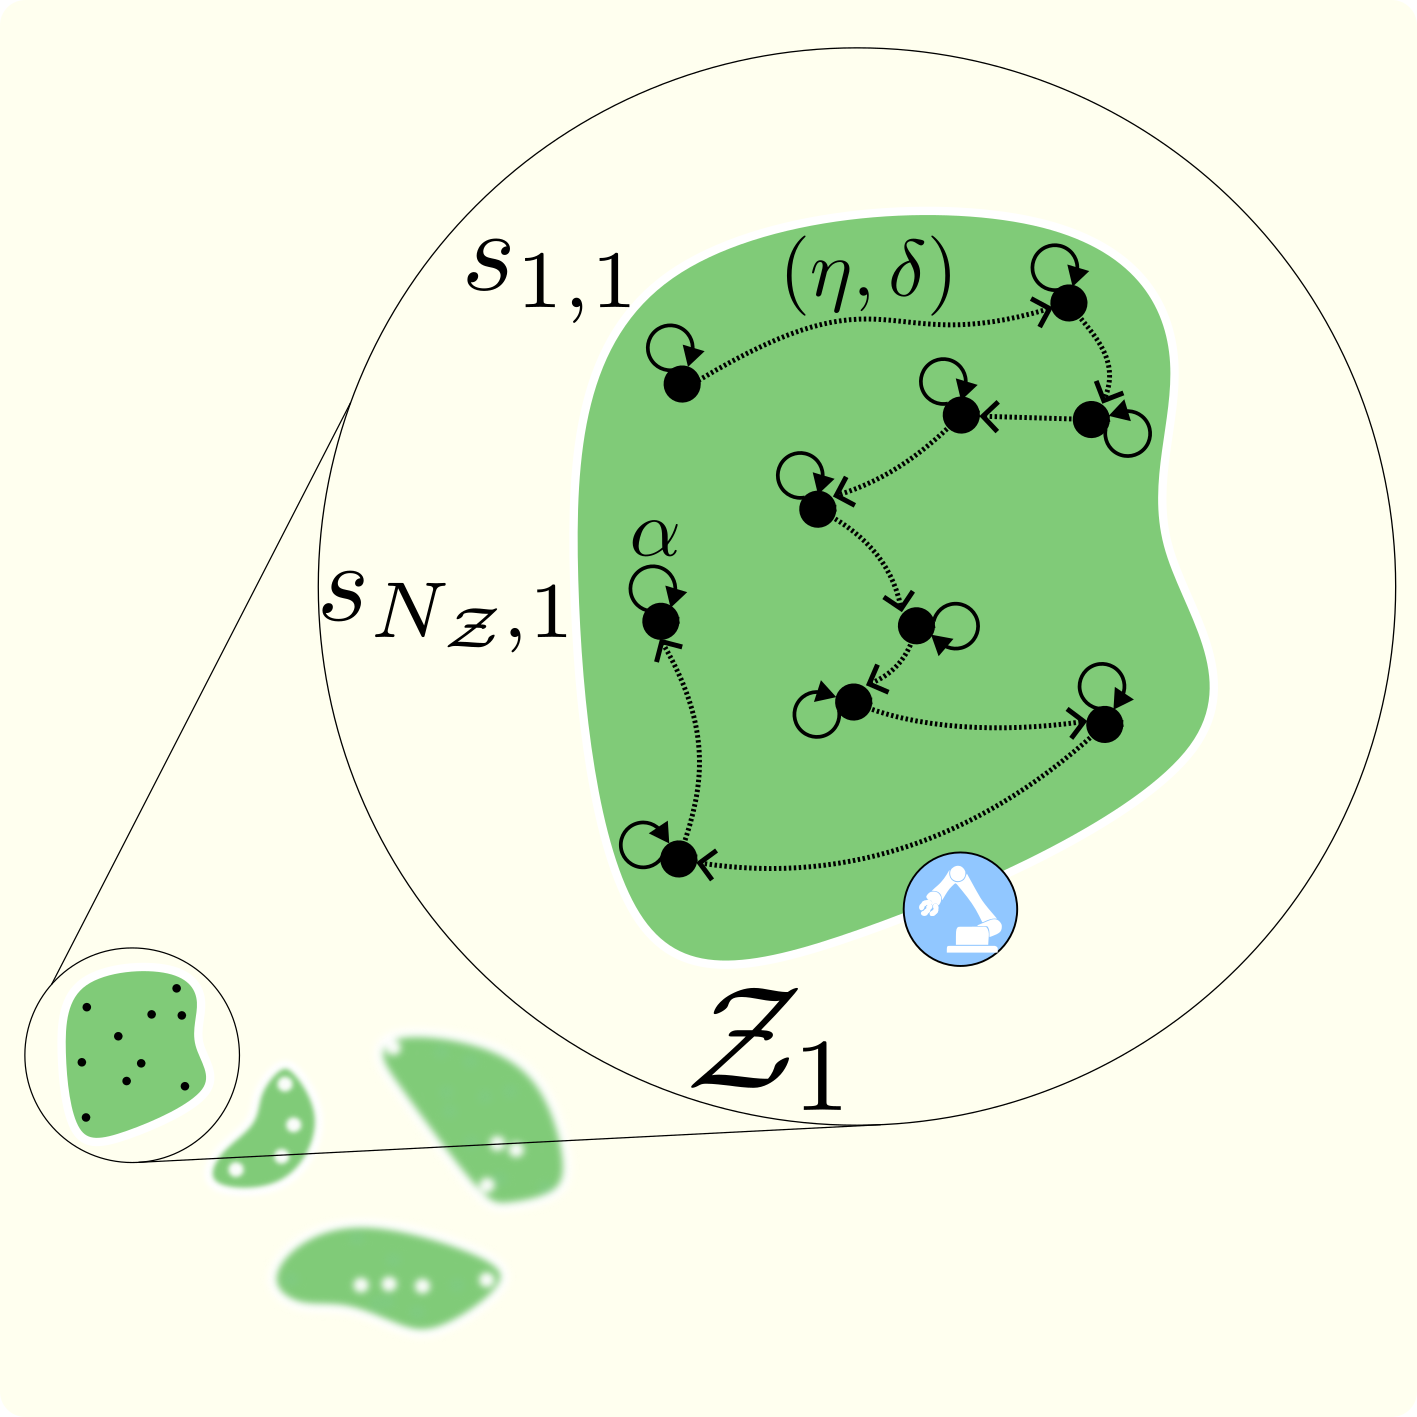
\includegraphics[width=0.95\columnwidth]{fig/intra_skill_learning.png}
	\caption{Incremental learning benefits from the significant similarity of skills belonging to the same cluster.}
	\label{fig:intra_skill_learning}
\end{figure}
% ---
% ---
\begin{figure*}[!htb]
	\centering
	\hspace*{\fill}
	\subfloat[]{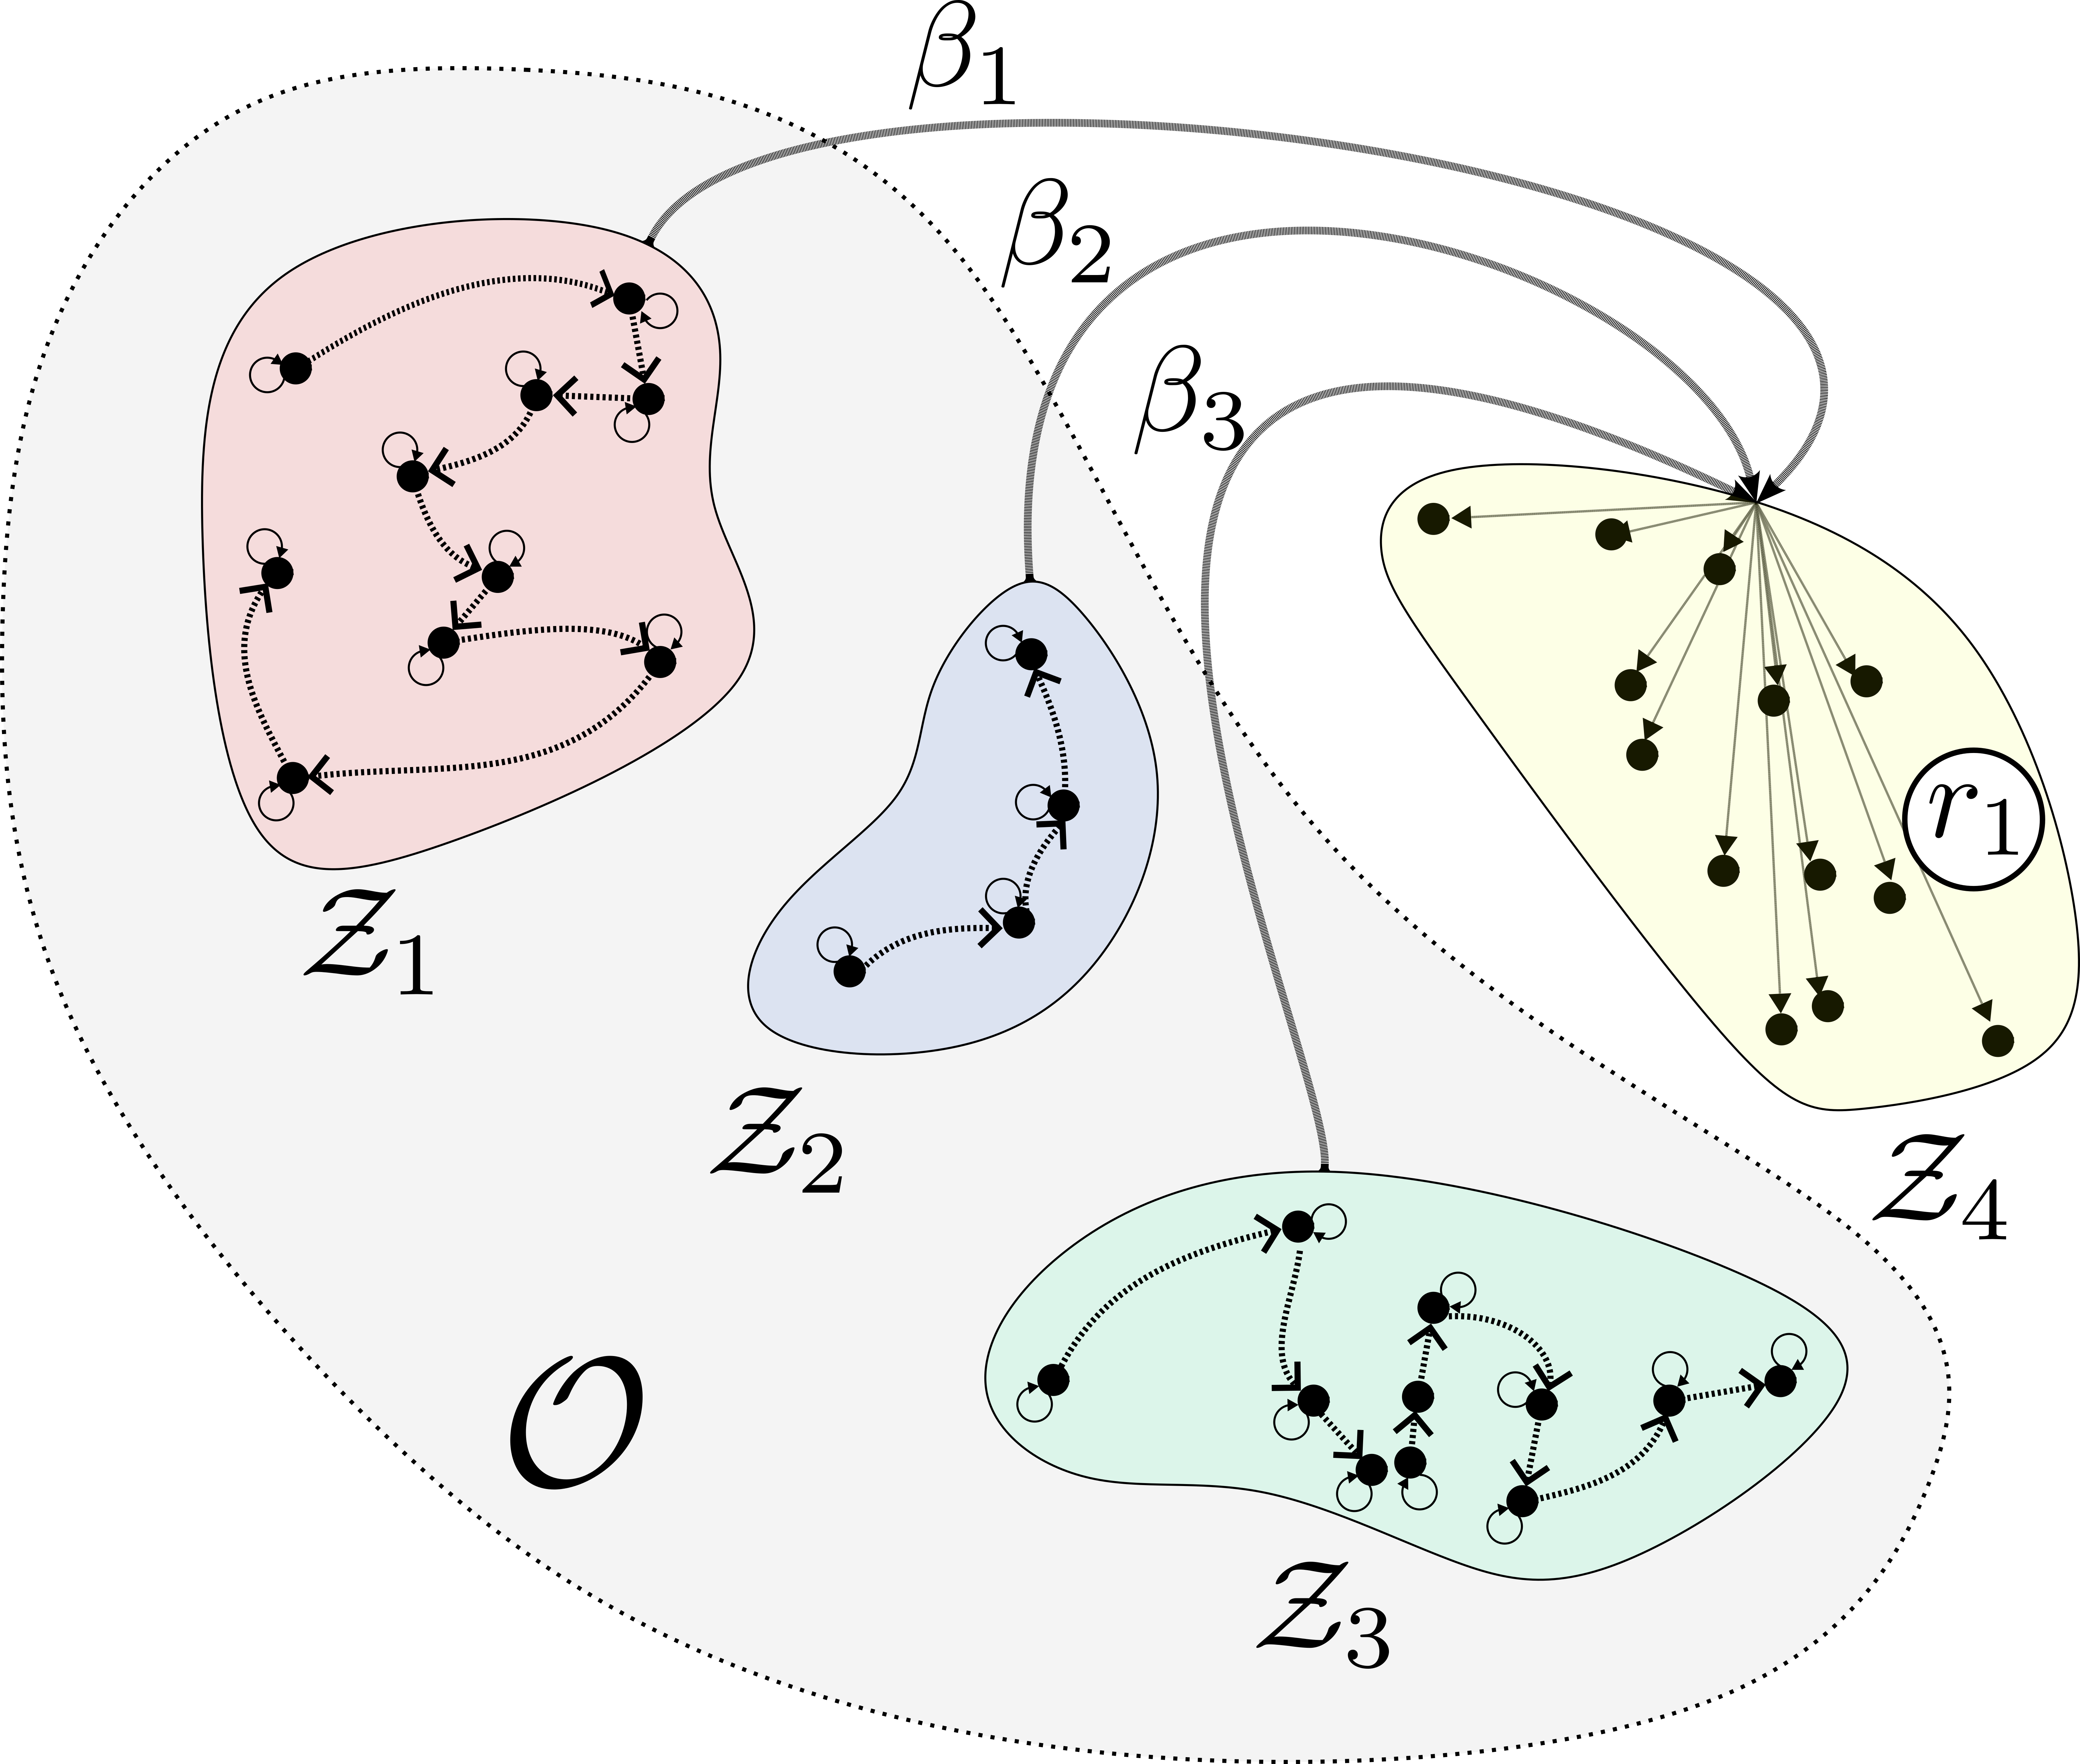
\includegraphics[width= 0.45\textwidth]{fig/cluster_to_cluster_knowledge_transfer.png} \label{fig:cluster_to_cluster_knowledge_transfer}}  
	\hfill	
	\subfloat[]{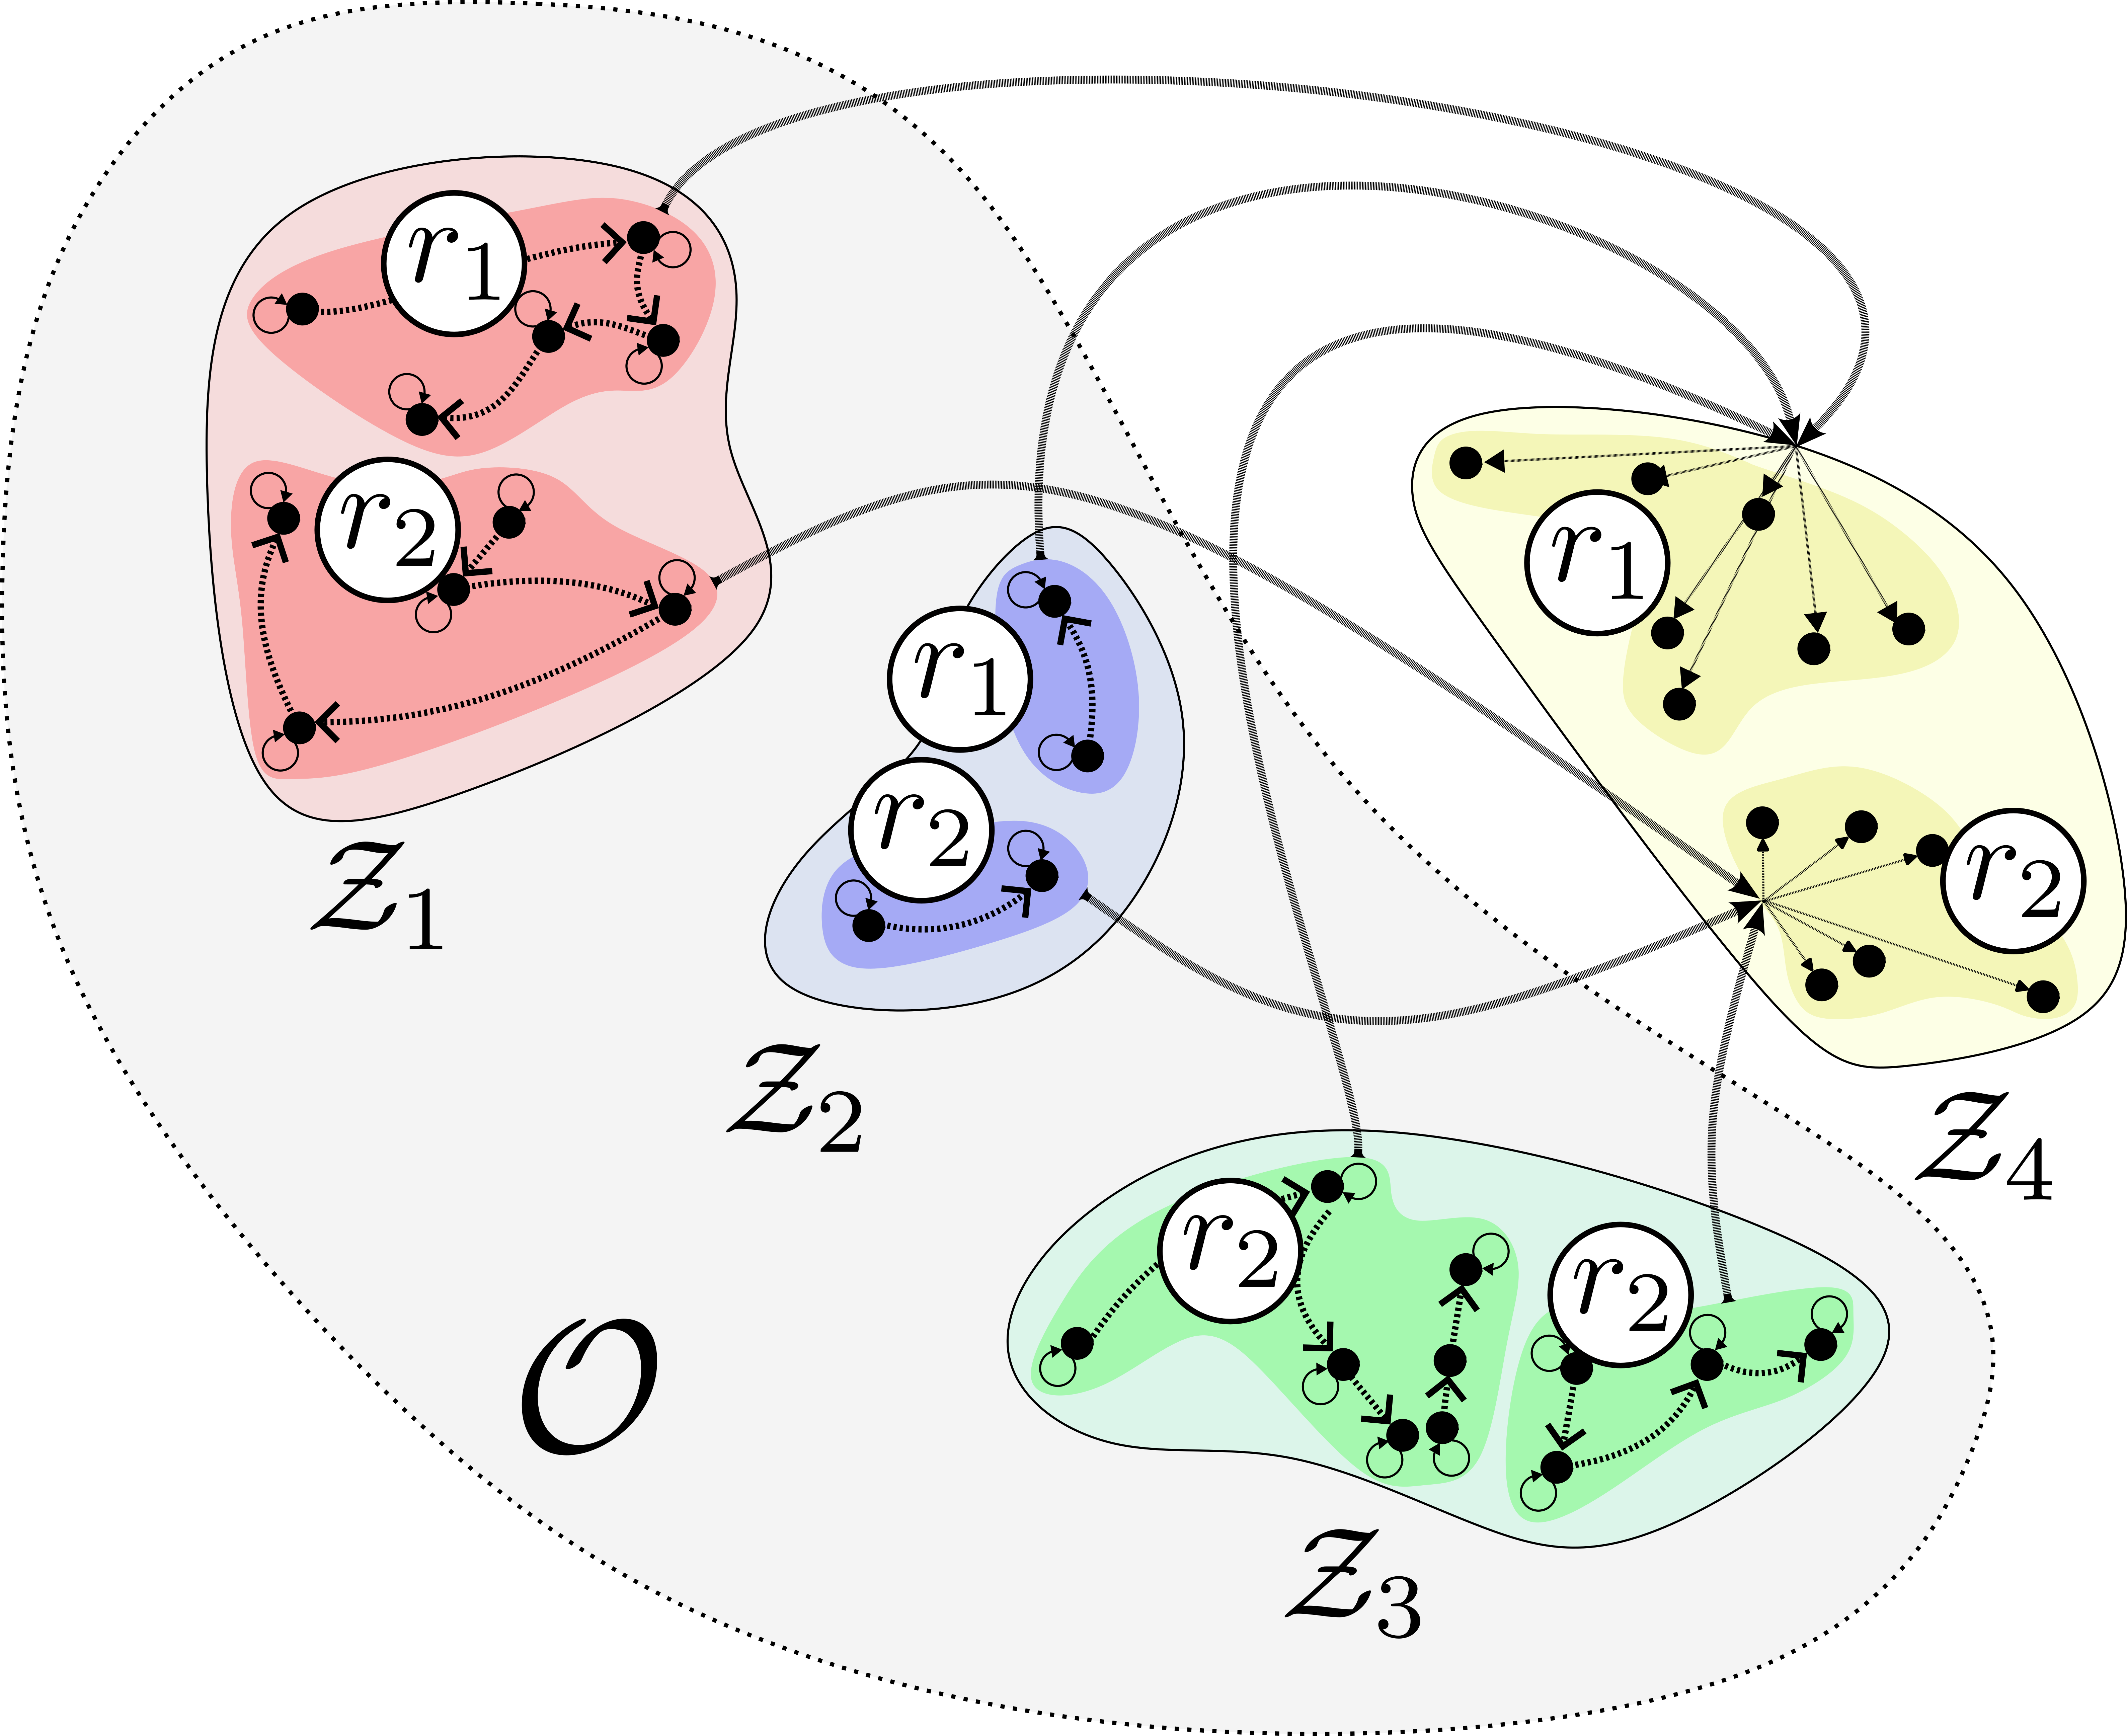
\includegraphics[width= 0.45\textwidth]{fig/cluster_to_cluster_knowledge_transfer_parallel.png} \label{fig:cluster_to_cluster_knowledge_transfer_parallel}}
	\hspace*{\fill}
	\caption[] {\label{fig:tranfer_learninhg} Transfer learning. \subref{fig:cluster_to_cluster_knowledge_transfer} Transfer of knowledge from different origin clusters to the target cluster,  \subref{fig:cluster_to_cluster_knowledge_transfer_parallel} using many robots (e.g. two robots $r_1$ and $r_2$) without knowledge exchange among them only subdivides the problem.}
\end{figure*}
% ---
% ---------------------------------------------------------------------------------------------------
\subsubsection{\textbf{Incremental Learning (IL)}}
It corresponds to the continuous aggregation and exchange of knowledge from \emph{intra-cluster} skills. Referring back to Asm.~\ref{assumption:skill_clustering}, the knowledge from skills belonging to a cluster ${\mathcal{Z}_k}$ can be be leveraged by an agent in virtue of their significant similarity. As depicted in Fig.~\ref{fig:intra_skill_learning}, a robot ($r_1$ in this case) learns every skill in $\mathcal{Z}_1$ with a rate $\alpha$ ---the self loops--- but also retains and uses the acquired knowledge to learn subsequent skills. The effect of incremental learning on the knowledge collection rate can be modeled to be directly proportional to the number of learned skills as
% ---
\begin{equation}\label{eq:f_function_incremental}
	f_{j,k}\left(N_{\zeta_k}\right) = -\alpha\left(\eta N_{\zeta_k} + 1 \right), 
\end{equation}
% ---
where $\eta>0$ represents the efficiency of knowledge exchange from $\zeta_k$ to $s_{j,k}$. Different potential models might be used to model the depletion of the initial remaining knowledge represented by $g_{j,k}\left(N_{\zeta_k}\right)$, e.g. a linear decay rate, our expectation is that, under the assumption that a learning strategy involving the ordering of skills according to similarity and their balanced distribution in the different clusters, $g_{j,k}\left(N_{\zeta_k}\right)$ might naturally resemble an exponential decay that is strongly dependent on $N_{\zeta_k}$. Such considerations motivate our choice of the following function
% ---
\begin{equation}\label{eq:g_function_incremental}
	g_{j,k}\left(N_{\zeta_k}\right) = e^{-\delta N_{\zeta_k}},
\end{equation}
%---
again with a factor $\delta>0$ controlling the rate at which the exponential converges. Similar to $\alpha$, using Asm.~\ref{assumption:cluster_size} $\delta$ can be defined as 
% ---
\begin{equation}\label{eq:delta}
	\delta = -\frac{1}{N_\mathcal{Z}}\text{log}(\epsilon).
\end{equation}
% ---
Essentially, such choice of $\delta$ implies that the remaining knowledge in a cluster after seeing all its skills is negligible. Via the exchange factors $(\eta,\delta)$, in incremental learning the knowledge about every new skill gets gradually increased by leveraging previous knowledge, resulting in
% ---
\begin{equation*}\label{eq:remaining_knowledge__IL}
	\bar{\sigma}^{(IL)}_{i,j}(n) = e^{-\alpha  \left(\eta N_{\zeta_k}+1\right) n} e^{-\delta N_{\zeta_k}}.
\end{equation*}
% ---
As the complexity $c_{j,k}$ of a skill can also be interpreted as the number of trial episodes required for the remaining knowledge to go below a threshold $\epsilon$; i.e.
% ---
\begin{equation*}
	\bar{\sigma}^{(IL)}_{i,j}(n) \Big \rvert_{n \ge c^{(IL)}_{j,k}} \leq \epsilon.
\end{equation*}
% ---
Then, under this scheme the complexity $c^{(IL)}_{j,k}$ to learn a new is skill in the cluster results in
%\begin{equation}\label{eq:complexity_IL}
%	c^{(I)}_{j,k} = -\frac{\text{log}(\epsilon)}{\alpha \eta (N_{\zeta_k}+ 1)}.
%\end{equation}
\begin{equation}\label{eq:complexity_IL}
	c^{(IL)}_{j,k} = -\frac{\text{log}(\epsilon) - \text{log}\left(\bar{\sigma}^{(IL)}_{j,k}(0)\right)}{\alpha (\eta N_{\zeta_k}+ 1)} = -\frac{\text{log}(\epsilon) + \delta N_{\zeta_k}}{\alpha (\eta N_{\zeta_k}+ 1)}  .
\end{equation}
% ---
The total number of trial episodes $ C_k $ that an agent following an incremental learning strategy needs to learn the $N_{\mathcal{Z}_k}$ skills in a cluster $ \mathcal{Z}_k $ is given by
% ---
\begin{align}\label{eq:total_episodes_incremental}
	\begin{split}
		C^{(IL)}_k &= \sum^{N_{\mathcal{Z}}}_{j=1} c^{(IL)}_{j,k}.
	\end{split}
\end{align}
% ---

\paragraph*{Multi-agent case}
If $m$ robots are used in parallel to divide the load of learning the tasks then
% ---
\begin{align}
	\begin{split}
		{}^{\lvert \rvert}C^{(IL)}_k &= \sum^{\frac{N_{\mathcal{Z}}}{m}}_{j=1} c^{(IL)}_{j,k}.
	\end{split}
\end{align}
% --
In essence, using $m$ robots without exchanging knowledge only subdivides the learning in every cluster into $m$ smaller problems \emph{without adding any additional benefit to the rate at which knowledge is acquired}. 

\subsubsection{\textbf{Transfer + Incremental Learning (TIL)}}
Transfer learning (TL) alone refers to the one-time \emph{inter-cluster} exchange of knowledge. Considering $\mathcal{K} = \{ \mathcal{Z}_k \}^{N_\mathcal{K}}_{k=1}$ to be the set of all available skill clusters, TL represents the exchange of knowledge from the skills learned in different \emph{origin} clusters $\mathcal{O} = \{ \mathcal{Z}_1,\mathcal{Z}_2,\ldots,\mathcal{Z}_{k-1} \}$ to the skills that will be learned in a \emph{destination} cluster $\mathcal{Z}_k$ (see Fig.~\ref{fig:cluster_to_cluster_knowledge_transfer}). Concretely, the effect that TL has on the skills of the destination cluster is the reduction of the initial remaining knowledge and the increase of the initial learning rate for all the skills in the $k$-th cluster via the parameter $\beta_k$; i.e.
% ---
\begin{equation}\label{eq:f_function_transfer}
	f_{j,k}\left(N_{\zeta_k}\right) = -\alpha \left( \frac{\eta N_{\zeta_k} + 1}{1 - \beta_k} \right),
\end{equation}
% ---
and
% ---
\begin{equation}\label{eq:g_function_transfer}
	g_{j,k}\left(N_{\zeta_k}\right) = (1-\beta_k) e^{-\delta N_{\zeta_k}}.
\end{equation}
%---
In essence, $\beta_k$ is the head start granted by knowledge transfer from other clusters to the skills in $\mathcal{Z}_k$. We argue that  $0<\beta_{k} < 1$ since it represents the \emph{aggregated} knowledge exchange factor from the different origin clusters $\mathcal{Z}_{c}$ to the target cluster $\mathcal{Z}_{k}$. Let $0<\beta_{c} < 1$ be the transfer contribution factor of a single origin cluster $\mathcal{Z}_c$. Additionally, consider that
% ---
\begin{equation}
	\sum\limits_{c=1}^{N_\mathcal{K}}\beta_{c} \leq 1,
\end{equation}
% --
as $1$ represents all the knowledge in $\mathcal{S}$. Asm.~\ref{assumption:cluster_transferability} implies that $\beta_c$ is equal for all the clusters. In this work we select $\beta_c = 1/N_\mathcal{K}$ for simplicity. The aggregated transfer factor $\beta_k$ is the sum of the individual factors from the already-visited clusters; i.e.
% ---
\begin{equation}\label{eq:beta_k_transfer}
	\beta_{k}= \left(k-1\right)\beta_c = \left(k-1\right)\frac{1}{N_\mathcal{K}}.
\end{equation}
% ---

Consequently, the remaining knowledge when transfer and incremental learning are used in conjunction is
% ---
\begin{equation}\label{eq:remaining_knowledge__ITL}
	\bar{\sigma}^{(TIL)}_{j,k}(n) = \left(1- \beta_k\right) e^{-\alpha  \left(\frac{ \eta N_{\zeta_k}+1}{1 - \beta_k}\right) n} e^{-\delta N_{\zeta_k}}.
\end{equation}
% ---
Similar to incremental learning, the complexity to learn a skill in transfer learning is
\begin{equation}\label{eq:skill_complexity_TL}
	c^{(TIL)}_{j,k} = -\frac{1 - \beta_{k}}{\alpha (\eta N_{\zeta_k}+ 1)}\left[\text{log}(\epsilon) + \delta N_{\zeta_k} - \text{log}(1 - \beta_{k})\right]
\end{equation}
% ---
and the total number of episodes  $ C_k $ that an agent requires to learn the $N_{\mathcal{Z}_k}$ skills is merely their sum
% ---
\begin{align}\label{eq:total_episodes_transfer}
	\begin{split}
		C^{(TIL)}_k &= \sum^{N_{\mathcal{Z}}}_{j=1} c^{(TIL)}_{j,k}.
	\end{split}
\end{align}
% --- 

\paragraph*{Multi-agent case}
If $m$ robots are used in parallel to divide the load of learning the tasks then, the transfer of knowledge from cluster to cluster is also divided by the number of robots, this implies that \eqref{eq:beta_k_transfer} changes to
% ---
\begin{equation}\label{eq:beta_k_transfer_parallel}
	{}^{\lvert \rvert}\beta_{k}= \frac{1}{m}\beta_{k}.
\end{equation}
% ---
Correspondingly, when using transfer learning in parallel $\beta_k$ is replaced by ${}^{\lvert \rvert}\beta_{k}$ in \eqref{eq:skill_complexity_TL}. Then, similar to IL, the total number of episodes to learn the skills in a cluster is
% ---
\begin{align}
	\begin{split}
		{}^{\lvert \rvert}C^{(TIL)}_k &= \sum^{\frac{N_{\mathcal{Z}}}{m}}_{j=1} c^{(TIL)}_{j,k}.
	\end{split}
\end{align}
% ---
This case is depicted on Fig.~\ref{fig:cluster_to_cluster_knowledge_transfer_parallel}, where two robots $ r_1$ and $r_2$ learn skills in four different clusters. The shaded areas are the subclusters of skills learned by each robot. Since they do not share knowledge between them, each robot has access only to the knowledge it has collected and cannot benefit from one another. 

% ---------------------------------------------------------------------------------------------------
\subsubsection{\textbf{Collective learning (CL)}}
As mentioned in Sec.~\ref{sec:intro}, EAI agents will be a core element of industrial, healthcare, and domestic ecosystems with advanced communication and remote processing capabilities. Given the anticipated legions of EAI agents executing and learning several different skills at any given time in those environments, it is immediately evident that the previous learning paradigms are not meant to exploit these large number of agents together with the advanced communication and processing infrastructure to take full advantage of the potential for concurrent knowledge exchange among the agents. Therefore, the use of isolated, incremental, and transfer learning by these many agents 
would directly aggravate computational demand (see \textbf{challenge 1} in Sec.~\ref{sec:robots_challenge}). As discussed in \cite{Kaelbling2020foundationefficientrobot} an leaning algorithm that would allow an agent to learn new tasks on-the-fly would need to be sample-efficient, generalizable, compositional, and (truly) incremental. Collective learning is the natural paradigm that meets this requirements exploiting the full communication potential of the networked EAI agents to leverage the real-time synergistic exchange and aggregation of collected knowledge to make the learning of tasks energy- and time-efficient.

To formalize this idea, let $ \left\lbrace \rho_i \right\rbrace_{i=1}^{m} $ be a set of robotic agents that defines a community of robots. In collective learning, the different robotic agents $ \rho_i $ develop and accumulate dynamically a common mind (body of knowledge) via networked interactions where individual experience, knowledge and skills are disseminated to all the other elements in the collective. Information flows vertically as previous knowledge is passed on, as well as horizontally by sharing concurrent experience between agents. Via these mechanisms, knowledge can be replicated, complimented and further developed. We take from \cite{Garavan2012CollectiveLearning} two notions central in collective learning that are applicable to the embodied AI agents:
% ---
\begin{enumerate}
	\item Capability to restructure and meet changing conditions
	\item Aggregation of skills, knowledge, and behaviors
\end{enumerate}
% ---
Collective learning contrasts with the previously discussed incremental learning in that a single agent $ r_i $ can aggregate only so much knowledge via trial and error and is limited by a sequential learning structure. Learning collectively, on the other hand, enforces parallelization of knowledge acquisition via the concurrent learning and sharing of all agents as they acquire new skills, knowledge. Moreover, collective learning involves not only the information acquisition, but also how this information is brought to use to form and develop knowledge. 

CL is not only a promising research direction but, in our opinion, has the potential to be a unifying solution to the grand challenges posed by embodied AI. Furthermore, by incorporating new mechanical designs as elements of the learning pipeline it is possible to iteratively evaluate the energy efficiency of proposed solutions and select the best ones as reference designs for future manufacturing processes with underlying learning, therefore, promoting a cyclical optimization towards a semi-optimal general design.
% ---
\begin{figure}[!th]
	\centering
	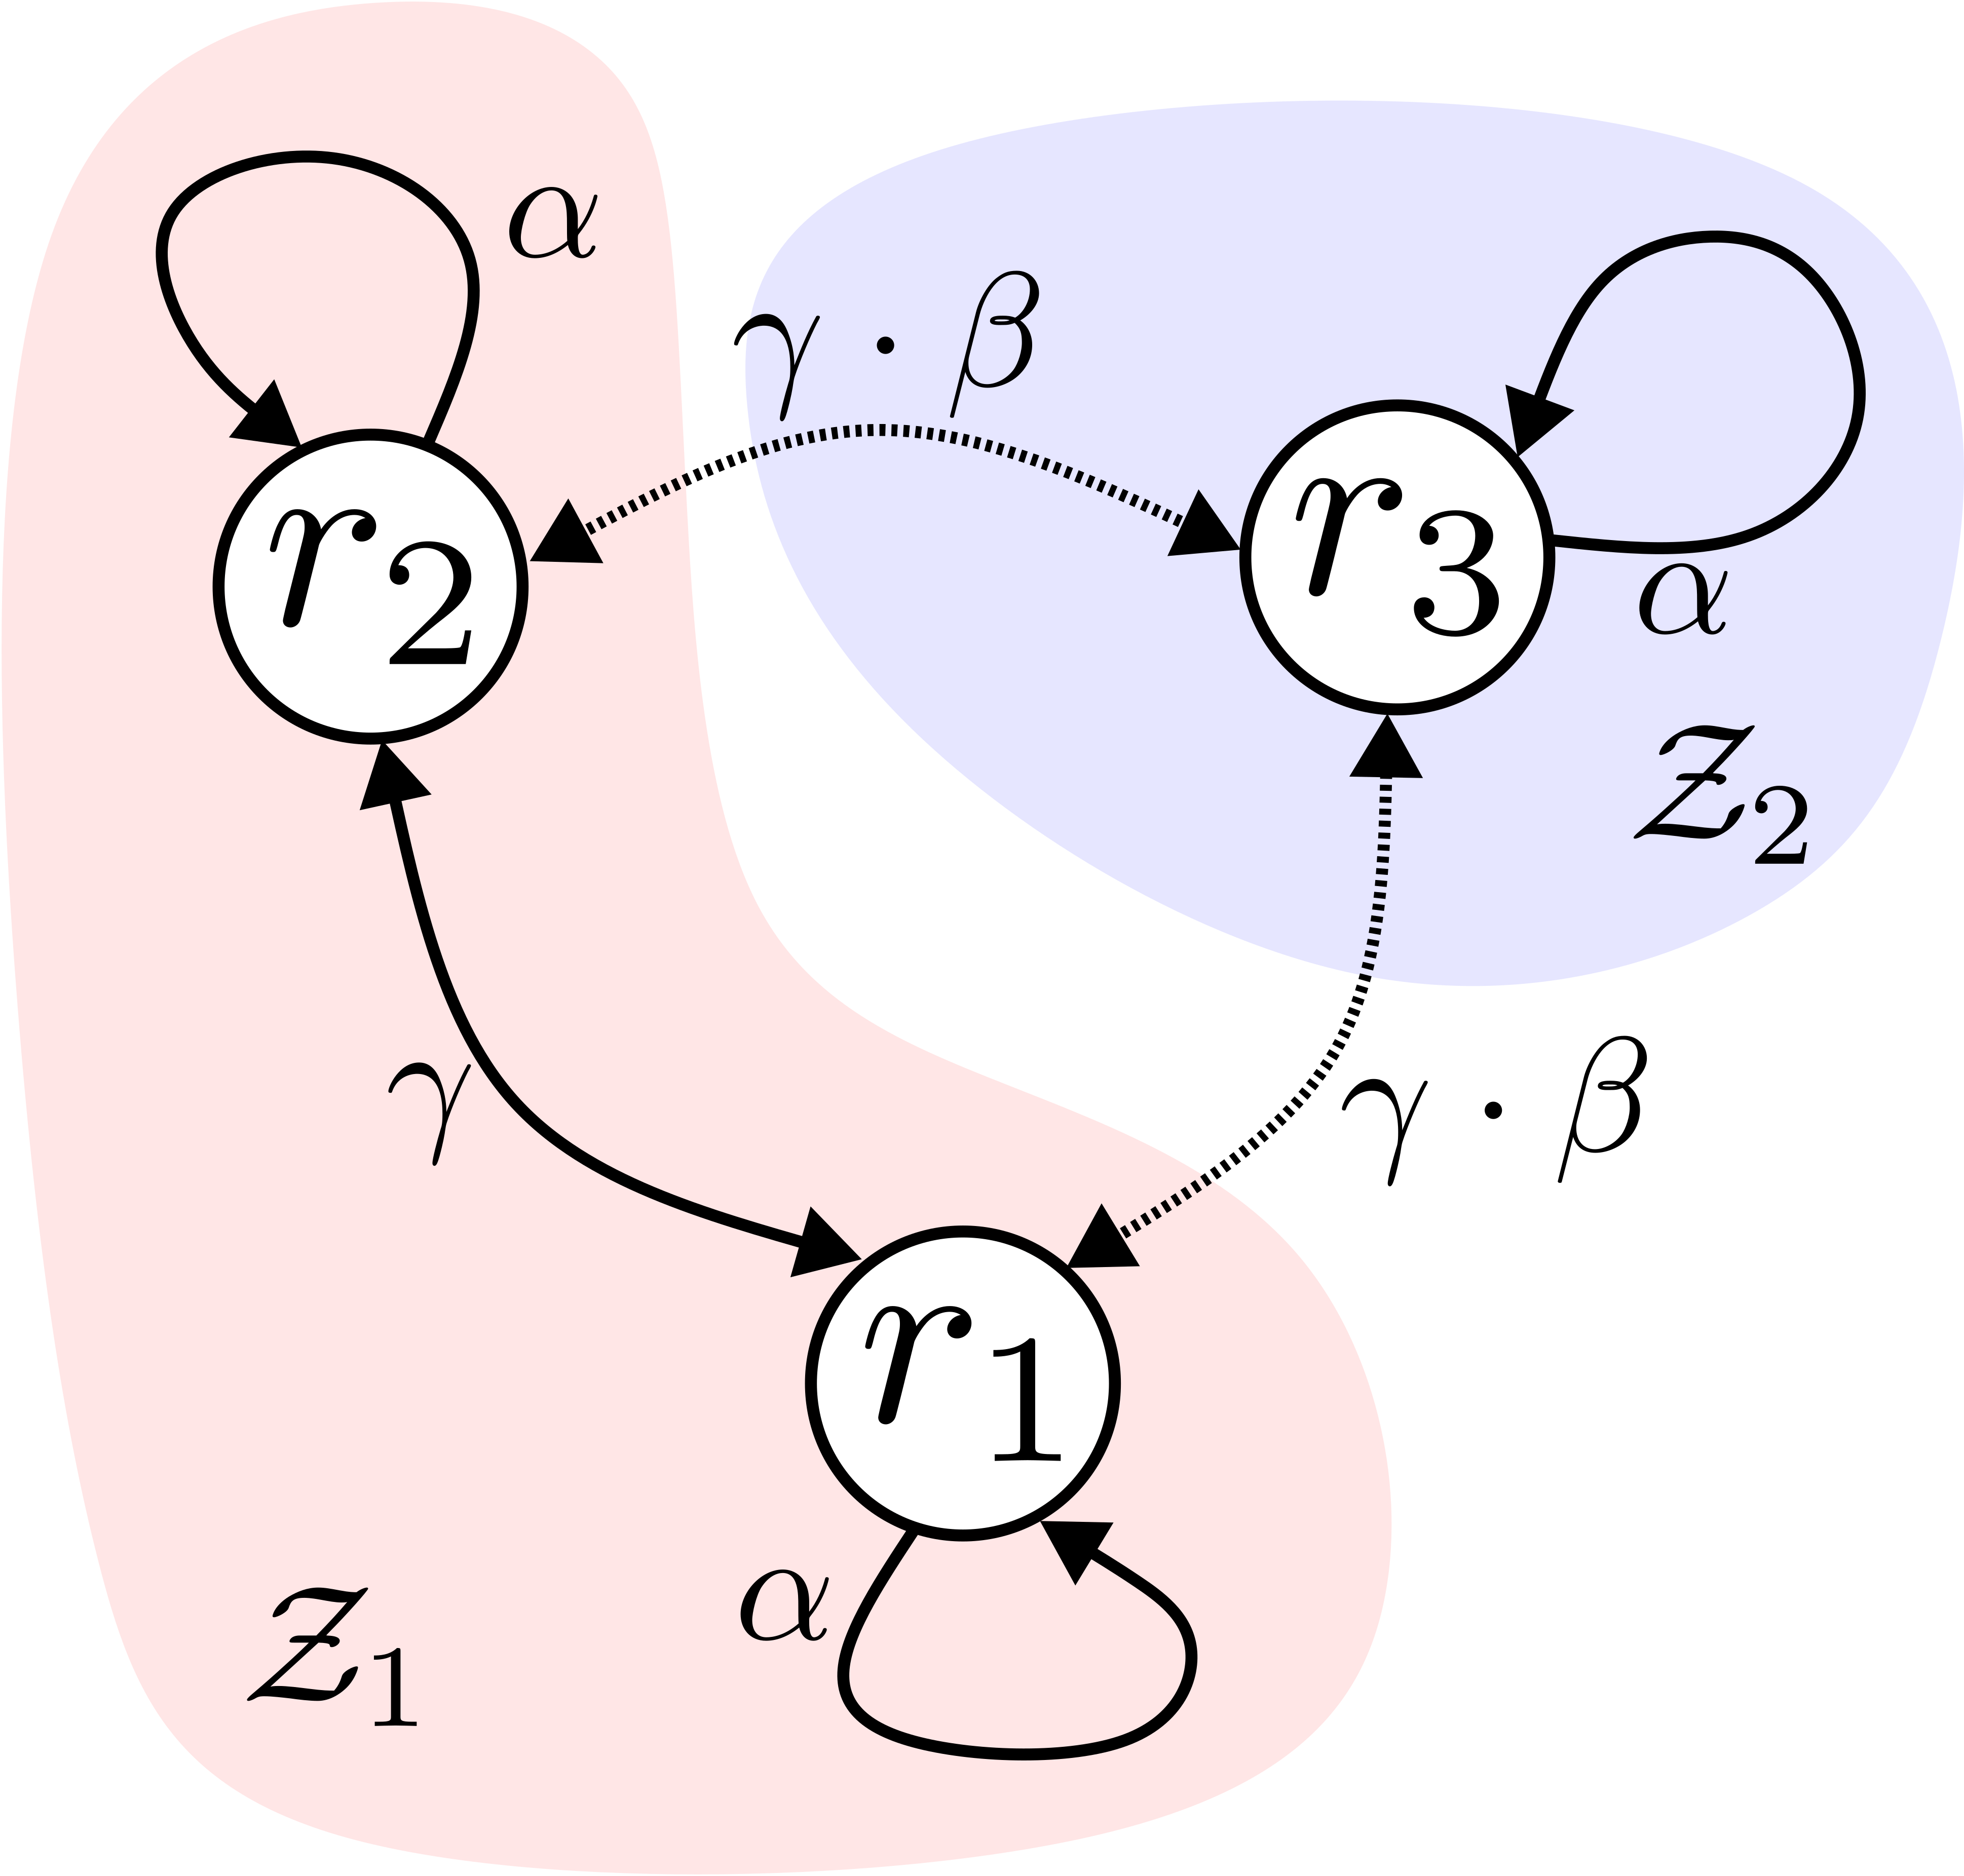
\includegraphics[width=0.7\columnwidth]{fig/cl_example_figure.png}
	\caption{Exchange of knowledge between EAI agents enables collective learning.}
	\label{fig:cl_example_figure}
\end{figure}
% ---

Unlike isolated and transfer learning, in this paradigm a batch of robots $\left \lbrace r_i \right \rbrace^m_{1}$ not only learn different skills concurrently but also exchange the acquired knowledge between each other and are actually able to leverage it. To enable CL, it is assumed that
\begin{itemize}
	\item an inter-agent communication protocol/infrastructure is in place that
	\item enables agents to concurrently exchange and integrate the self-acquired and received knowledge to
	\item incrementally speed up the learning of all the agents as a whole.
\end{itemize}
% ---
As a result, the intra- and inter-cluster knowledge transfer is possible. Naturally, the CL paradigm involves a complex scheduling problem to determine the optimal skill distribution and inter-agent knowledge sharing strategy. Since we have not tackled this problem yet, we ground the subsequent discussion on Assumptions~\ref{assumption:average_behavior}, \ref{assumption:agent_similarity},~\ref{assumption:cluster_size}, and~\ref{assumption:cluster_transferability} that suggest an average behavior given a suitable scheduling.

Fig.~\ref{fig:cl_example_figure} illustrates the CL concept, where the self loop represents the dynamics of a single robot learning (at a rate $\alpha$). The exchange of knowledge across agents is represented via the cross-couplings weighted by a parameter $\gamma$ that models how efficient is the bidirectional pairwise knowledge exchange. Similar to transfer learning, if two robots exchange knowledge about skills with low similarity (i.e. skills in different clusters), then $\gamma$ is scaled by the inter-cluster transferability parameter $\beta$. In CL \eqref{eq:simple_knowledge_dynamics} is extended to 
% ---
\begin{subequations}\label{eq:collective_knowledge_dynamics}
	\begin{alignat}{2}
		\dot{\bar{\bm{\sigma}}}^{(CL)}_{j,k}\left(n\right) &= \overbrace{\left[  f_{j,k}\left(N_{\zeta_k},r\right) \bm{I} + \gamma \bm{A} \odot \bm{B}  \right]}^{\bar{\bm{A}}\left(N_{\zeta_k}\right)} \bar{\bm{\sigma}}^{(CL)}_{j,k}\left(n\right)\\
		\bar{\bm{\sigma}}^{(CL)}_{j,k}(0) &= g_{j,k}\left( N_{\zeta_k}, r\right) \bm{I},
	\end{alignat}
\end{subequations}
% ---
where $r=m$ is the number of robots that exchange knowledge among them. This implies that now $\bar{\bm{\sigma}}^{}_{j,k} \in \mathbb{R}^r$ is a vector that represents the dynamics of the remaining knowledge of all the $m$ skills being concurrently learned. $\bm{A} \in \mathbb{R}^{r \times r}$ is a zero-diagonal symmetric adjacency matrix whose entry $(\bm{A})_{i,j} = 1$ if robot $i$ exchanges knowledge with robot $j$ and $(\bm{A})_{i,j} = 0$ if it does not. The term $\gamma \in \mathbb{R}_+ $ weighs the knowledge exchange strength among robots. Furthermore, since there may be robots learning skills in different clusters at the same time, the matrix $\bm{B}$, whose entries are $\left(\bm{B}\right)_{i,j} \in \left \lbrace 1, \beta_{k} \right \rbrace$, with
% ---
\begin{equation}
	%\beta_{k} = 1/N_\mathcal{K}, 
	\beta_{k} = r\frac{ N_{\zeta_k}}{N_\mathcal{S}}, 
\end{equation}
% ---
scales down the knowledge contributions between robots from different clusters. Finally, the operator $\odot$ represents the Hadamard product of matrices. The functions $ f(\cdot)$ and $g(\cdot)$ are now also dependent on the number of robots that exchange knowledge, which directly impacts the number of skills that enter $\zeta_k$ after a learning cycle; i.e.
% ---
\begin{equation}\label{eq:f_function_collective}
	f_{j,k}\left(N_{\zeta_k},r\right) = -\alpha \left( \frac{\eta r N_{\zeta_k} + 1}{1 - \beta_k} \right),
\end{equation}
% ---
and
% ---
\begin{equation}\label{eq:g_function_collective}
	g_{j,k}\left(N_{\zeta_k},r\right) = (1-\beta_k) e^{-\delta r N_{\zeta_k}}.
\end{equation}
%---
Some considerations need to be taken when selecting the value of $\gamma$ given that the dynamics matrix of the collective system
% ---
\begin{equation}
	\bar{\bm{A}}\left(N_{\zeta_k}\right) = f\left(N_{\zeta_k},r\right) \bm{I} + \gamma \bm{A} \odot \bm{B} 
\end{equation} 
% ---
exhibits a dependency on the number of seen skills $N_{\zeta_k}$, which is directly influenced by the number of robots $r$ in the collective. Yet, it can be proven that there is a coupling strength $\gamma$ for a given connectivity $\bm{A}$ that ensures that the remaining knowledge for all skills converges asymptotically to zero.

\TODO \textcolor{red}{is there an approximation of the convergence rate of all the skills?}






% ===================================================================================================
%                                                 |                                                 |
%                                                 |                                                 |
% -------------------------------------------- SECTION ---------------------------------------------|
%                                                 |                                                 |
%                                                 |                                                 |
% ===================================================================================================
% ===================================================================================================
%                                                 |                                                 |
%                                                 |                                                 |
% -------------------------------------------- SECTION ---------------------------------------------|
%                                                 |                                                 |
%                                                 |                                                 |
% ===================================================================================================
\section{Use case: Smart factory}\label{sec_use_case}
% ---
%\begin{figure*}[!h]
%	\centering
%	\hspace*{\fill}
%	\subfloat[]{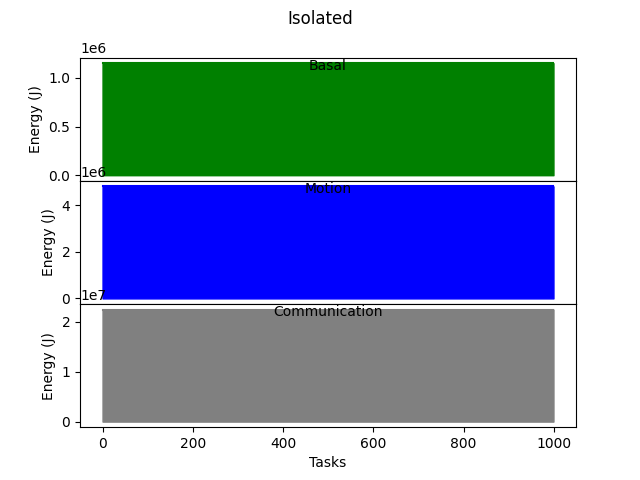
\includegraphics[width= 0.90\columnwidth]{fig/isolated_corrected.png} \label{fig:iso_energy}}
%	\hfill
%	\subfloat[]{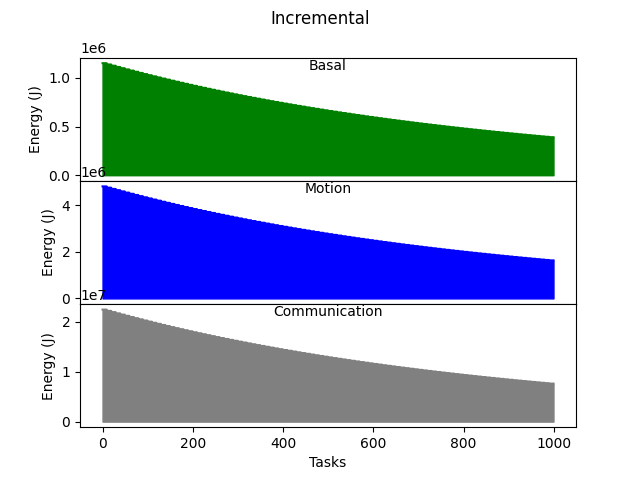
\includegraphics[width= 0.90\columnwidth]{fig/incremental_corrected.png} \label{fig:itl_energy}}
%	\hspace*{\fill}
%	\\%[-2ex]
%	\hspace*{\fill}
%	\subfloat[]{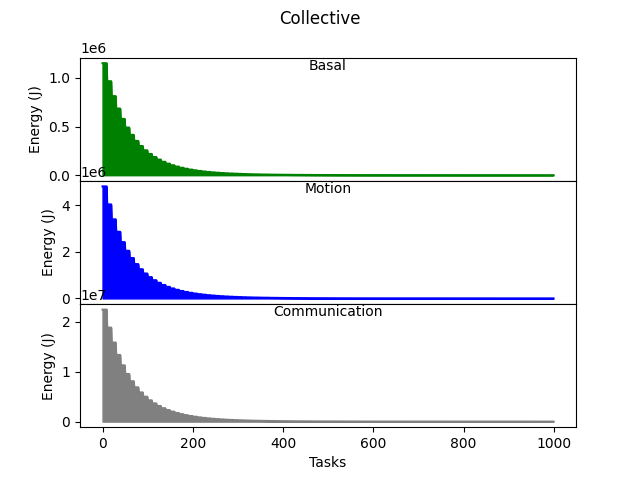
\includegraphics[width= 0.9\columnwidth]{fig/collective_corrected.png}\label{fig:cl_energy}}
%	\hfill    
%	\subfloat[]{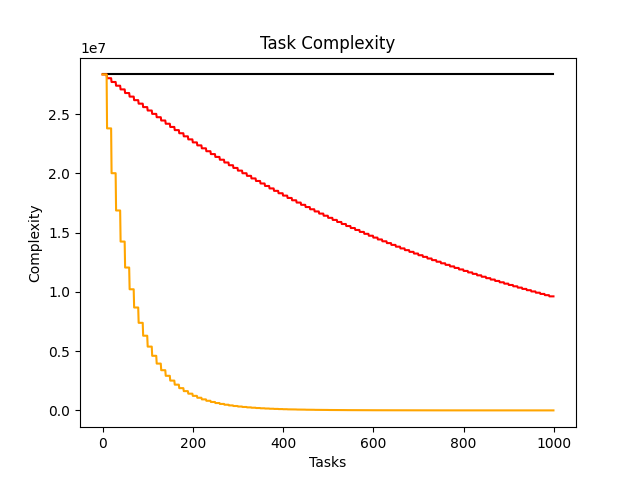
\includegraphics[width= 0.9\columnwidth]{fig/task_complexity.png}\label{fig:use_case_complexity}}
%	\hspace*{\fill}    
%	\caption[] {\label{fig:use_case_results} Energy expenditure per task: \subref{fig:iso_energy} isolated learning, \subref{fig:itl_energy} incremental+transfer learning,  \subref{fig:cl_energy} collective learning. \subref{fig:use_case_complexity} Scaling of the task complexity.}
%\end{figure*}
% ---
The goal of this section is to forecast the energy demand that EAI agents following the learning paradigms discussed in Sec.~\ref{sec:learning_paradigms} would have in a prototypical instance of a hypothetical smart factory. In this mock factory a pool $\mathcal{S}$ of $N_\mathcal{S}= 512$ industry relevant skills is divided into $N_\mathcal{K}=4$ clusters of $N_\mathcal{Z} = 128$ skills each. Additionally, consider that $m=32$ robots are available to learn the skills and that a skill is considered learned once the remaining knowledge goes below $\epsilon = 0.01$. For all the skills, the fundamental skill complexity is $c_0 = 100$ episodes.
% whose purpose is to execute a series of tasks, drawn from a pool $ \mathcal{T} $ of . In the example we consider \hl{a set of $N_{\mathcal{T}}=1,000$ related and similar tasks}; that is $ \mathcal{T}=\left\lbrace \tau_1,\ldots, \tau_{1000} \right\rbrace$, where we assume $ \tau_i \sim \tau_j $. These tasks will need to be learned by an embodied AI agent so that they can be executed and used in production. We will explore what would be the consequences of the isolated (what we call inefficient) learning paradigm and the envisioned, and arguably desired, collective learning paradigm. 

The power in \eqref{eq:energy_per_episode} is composed by the sum of the power required for basal processes, the power for motion and interaction, and the power for computation and communication; i.e.
% ---
\begin{equation}
    P_0 = P_{BEE}+P_{MIE} + P_{CCE}.
\end{equation}
% ---
To choose $P_{BEE}$, we consider that the smart factory will be populated with state-of-the-art cobots, like the Franka Emika Panda, which requires a typical power of about $\unit[72]{W}$. To approximate $P_{MIE}$, we use the fact that, in demanding tasks, the power demand of the cobot can go up to a maximum of about $ \unit[300] {W} $. Finally, to determine $P_{CCE}$, we make the assumption that, to deal with the computing effort that learning new skills will have on the robots' local processors, the smart factory will delegate the computational burden to a remote computing unit (i.e. cloud computing). Thus, we take as reference the work in \cite{Strubell2019EnergyAP}, where a state-of-the-art machine learning algorithm executed in a cluster required $\unit[1,415.78]{W}$ to solve a task. Additionally, without loss of generality, we can assume that each trial episode takes $\Delta t = 60$ seconds to execute. Using these reference values, we can estimate that, when learning a skill, a trial episode has en energetic demand of:
% ---
\begin{equation}
	e_0 = P_0 \Delta t = \left(70 + 300 + 1,415.78\right) \left(60\right) \approx 105~\text{kJ}
\end{equation}
% ---
Regarding the knowledge exchange efficiency constants, they are chosen as follows
% ---
% ---
\begin{itemize}
	\item $\alpha =  0.0461$ (in accordance to \eqref{eq:isolated_learning_rate})
	\item $\delta =  0.0360$ (see \eqref{eq:delta})
	\item $\eta= 0.1$
\end{itemize} 
% ---
%\begin{align}\label{eq:transfer_constants}¸
%\begin{split}
%    \alpha &=1\times10^{-3}\\
%    \beta &=1\times10^{-5}\\
%    \gamma &=1\times10^{-7}    
%\end{split}
%\end{align}
% ---
%Finally, we assume that each episode $n$ contains $k=10,000$ iterations.

% ===================================================================================================

%\subsection{Summary}
%
%The equation for incremental learning is equivalent to \eqref{eq:knowledge_exponential_form} with $r=1$ since no inter-agent exchange of knowledge occurs and $\beta_k = 0$,¸ as knowledge from other cluster cannot be used.
% ---
%\begin{figure*}[!th]
%	\centering
%	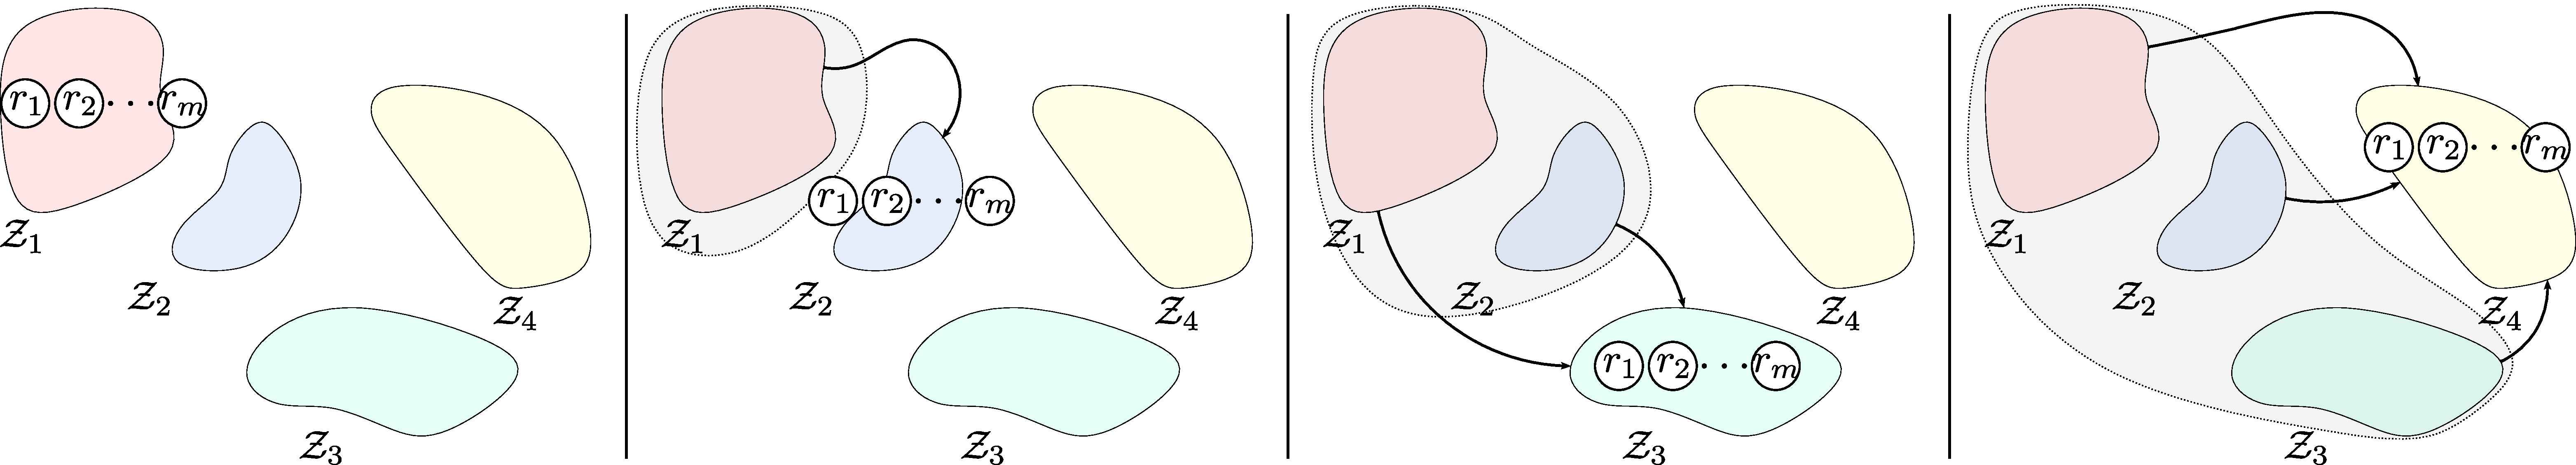
\includegraphics[width=0.95\textwidth]{fig/cluster_learning_sequence.pdf}
%	\caption{The sequence followed to learn the clusters.}
%	\label{fig:cluster_learning_sequence}
%\end{figure*}
% ---
%---
\begin{figure*}[!t]
	\centering
	\hspace*{\fill}
	\subfloat[]{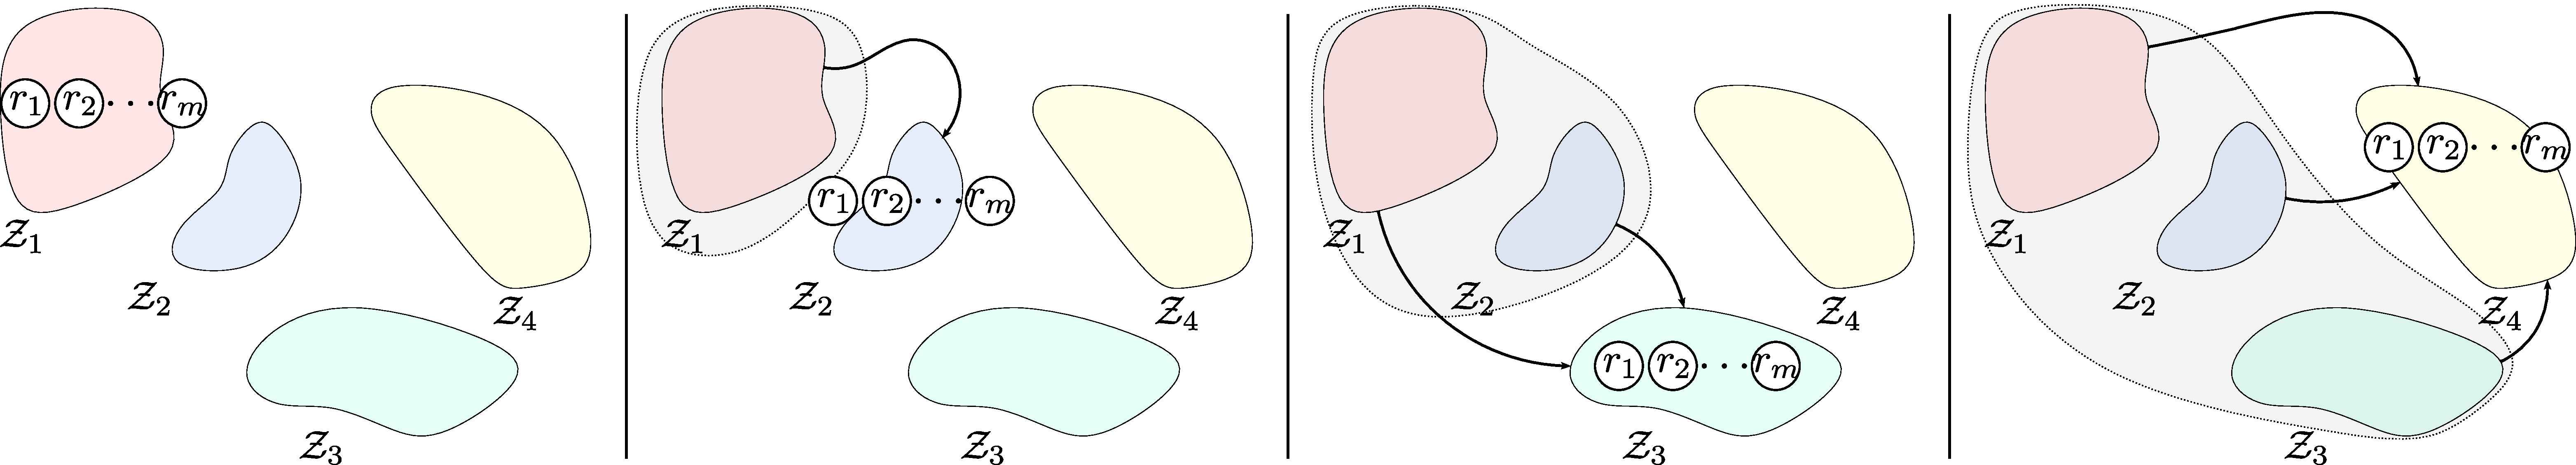
\includegraphics[width= 0.8\textwidth]{fig/cluster_learning_sequence.pdf} \label{fig:cluster_learning_sequence}}
	\hspace*{\fill}
	\\	
	\hspace*{\fill}
	\subfloat[]{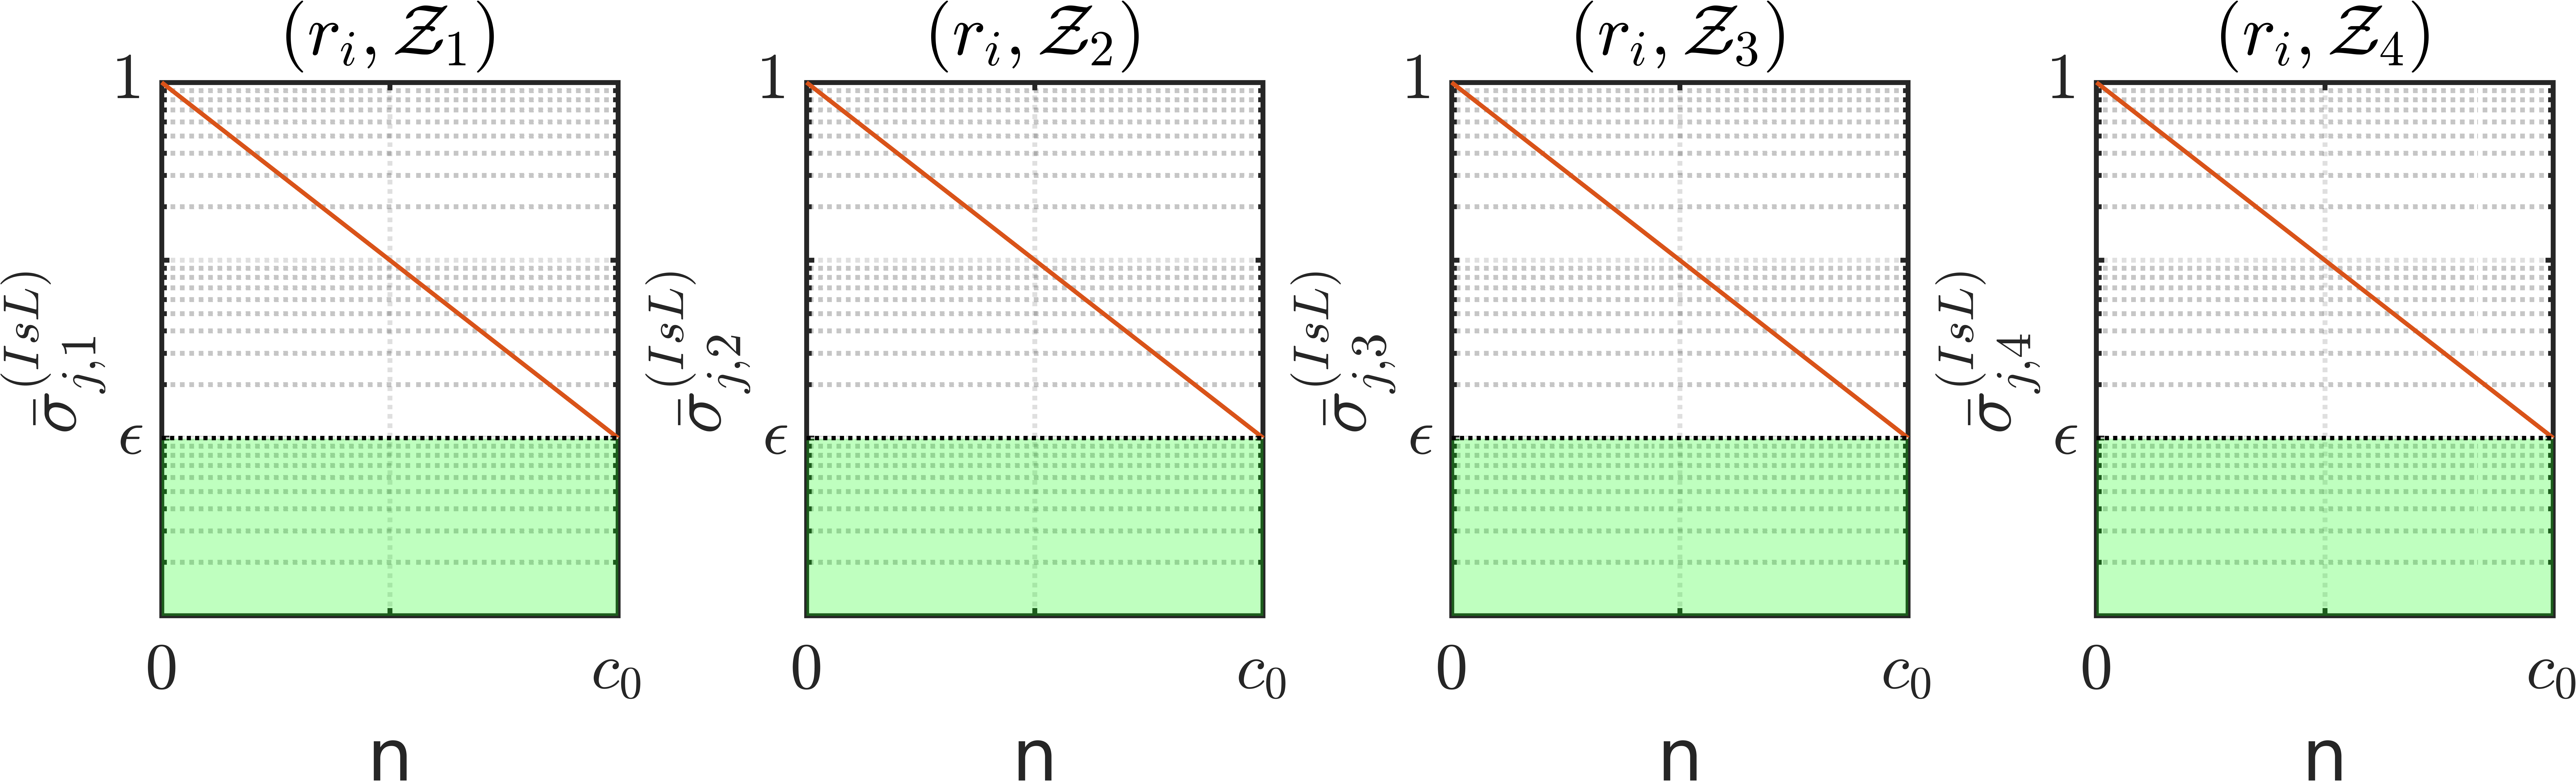
\includegraphics[width= 0.8\textwidth]{fig/dynamics_isolated_learning.pdf} \label{fig:dynamics_isolated_learning}}  
	\hspace*{\fill}
	\\	
	\hspace*{\fill}
	\subfloat[]{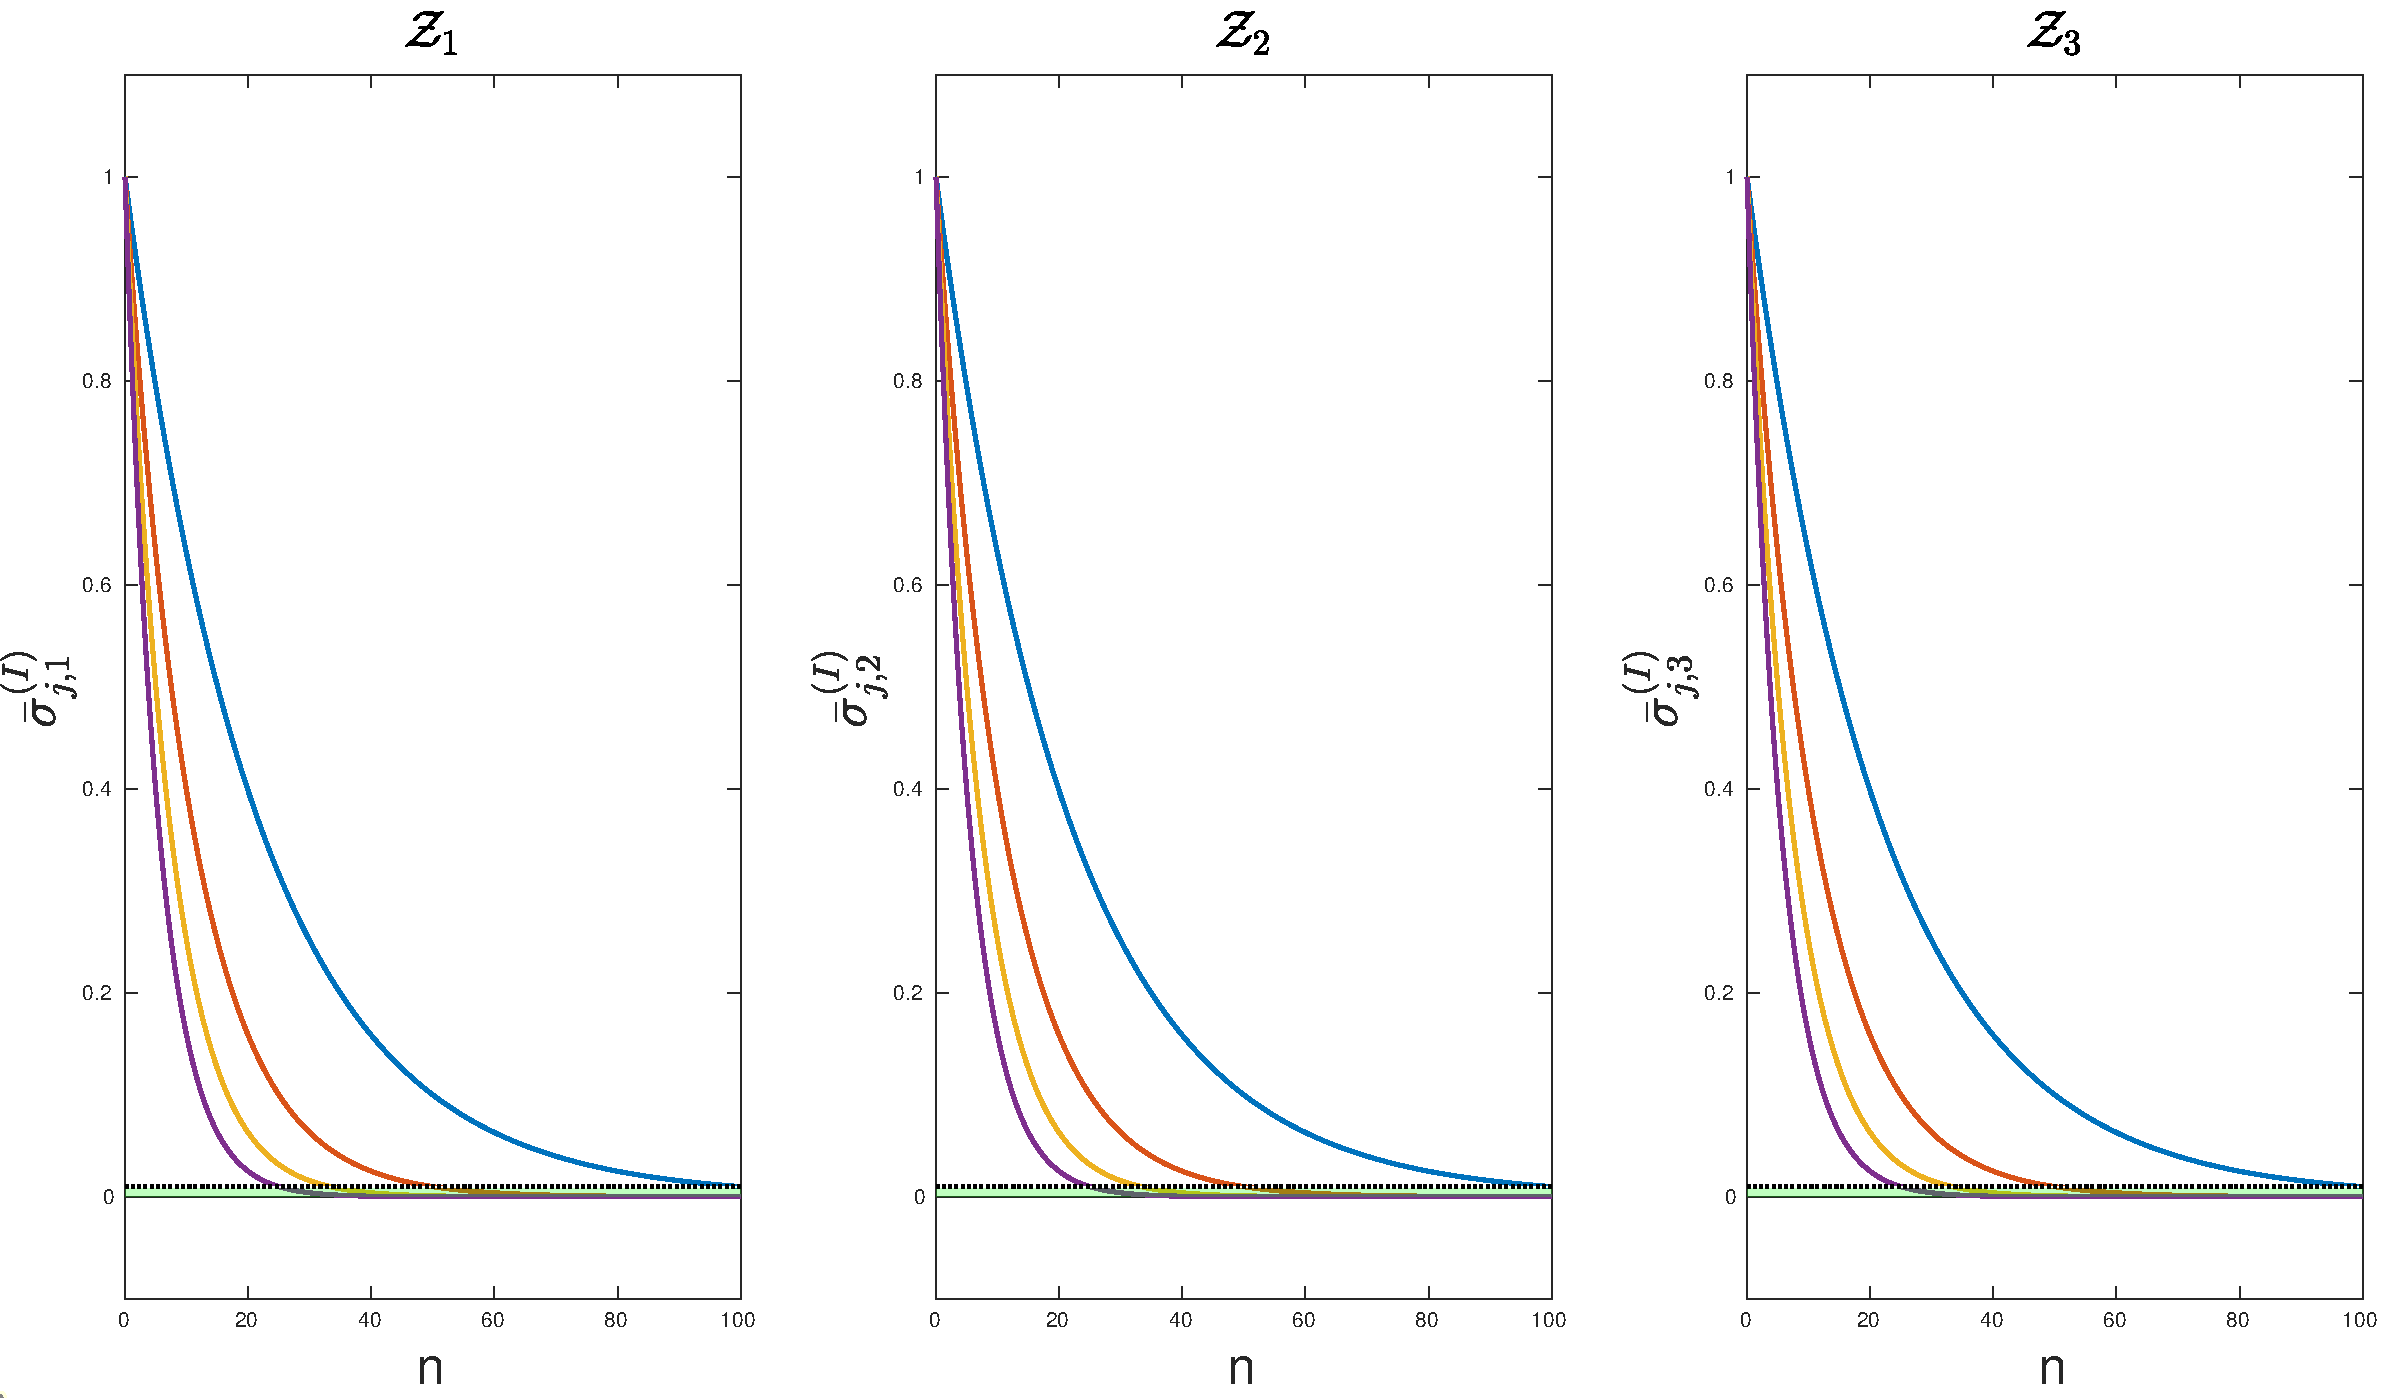
\includegraphics[width= 0.8\textwidth]{fig/dynamics_incremental_learning.pdf} \label{fig:dynamics_incremental_learning}}  
	\hspace*{\fill}	
	\\
	\hspace*{\fill}
	\subfloat[]{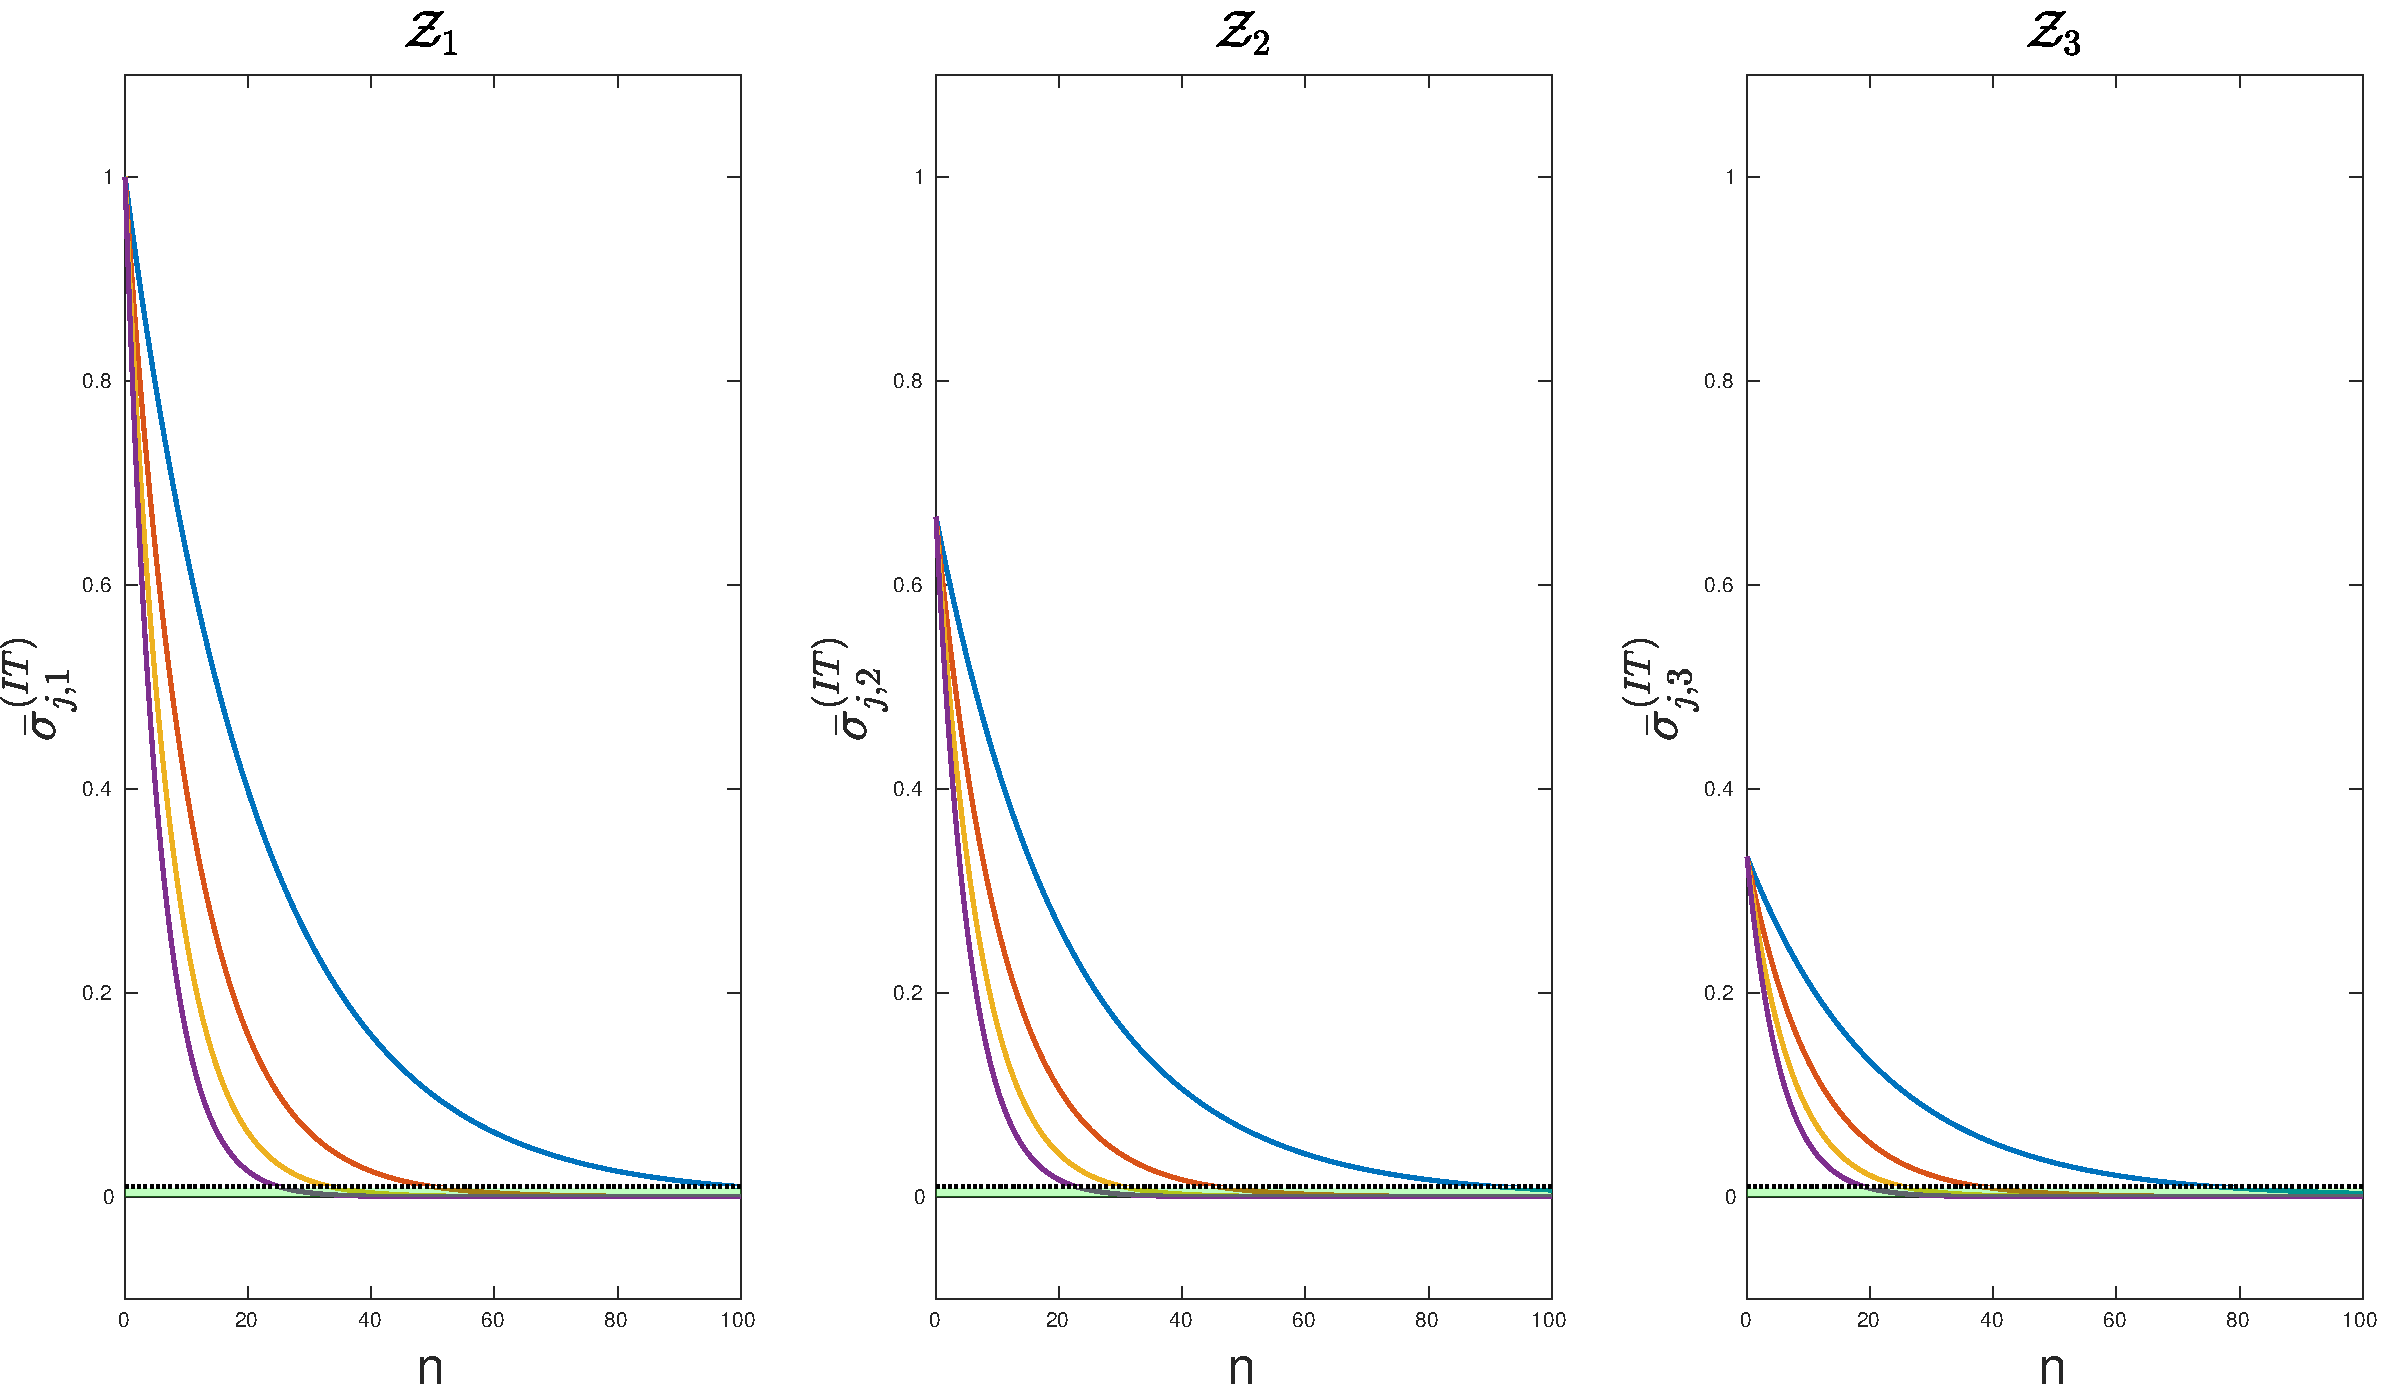
\includegraphics[width= 0.8\textwidth]{fig/dynamics_incremental_transfer_learning.pdf} \label{fig:dynamics_incremental_transfer_learning}}  
	\hspace*{\fill}
	\\
	\hspace*{\fill}
	\subfloat[]{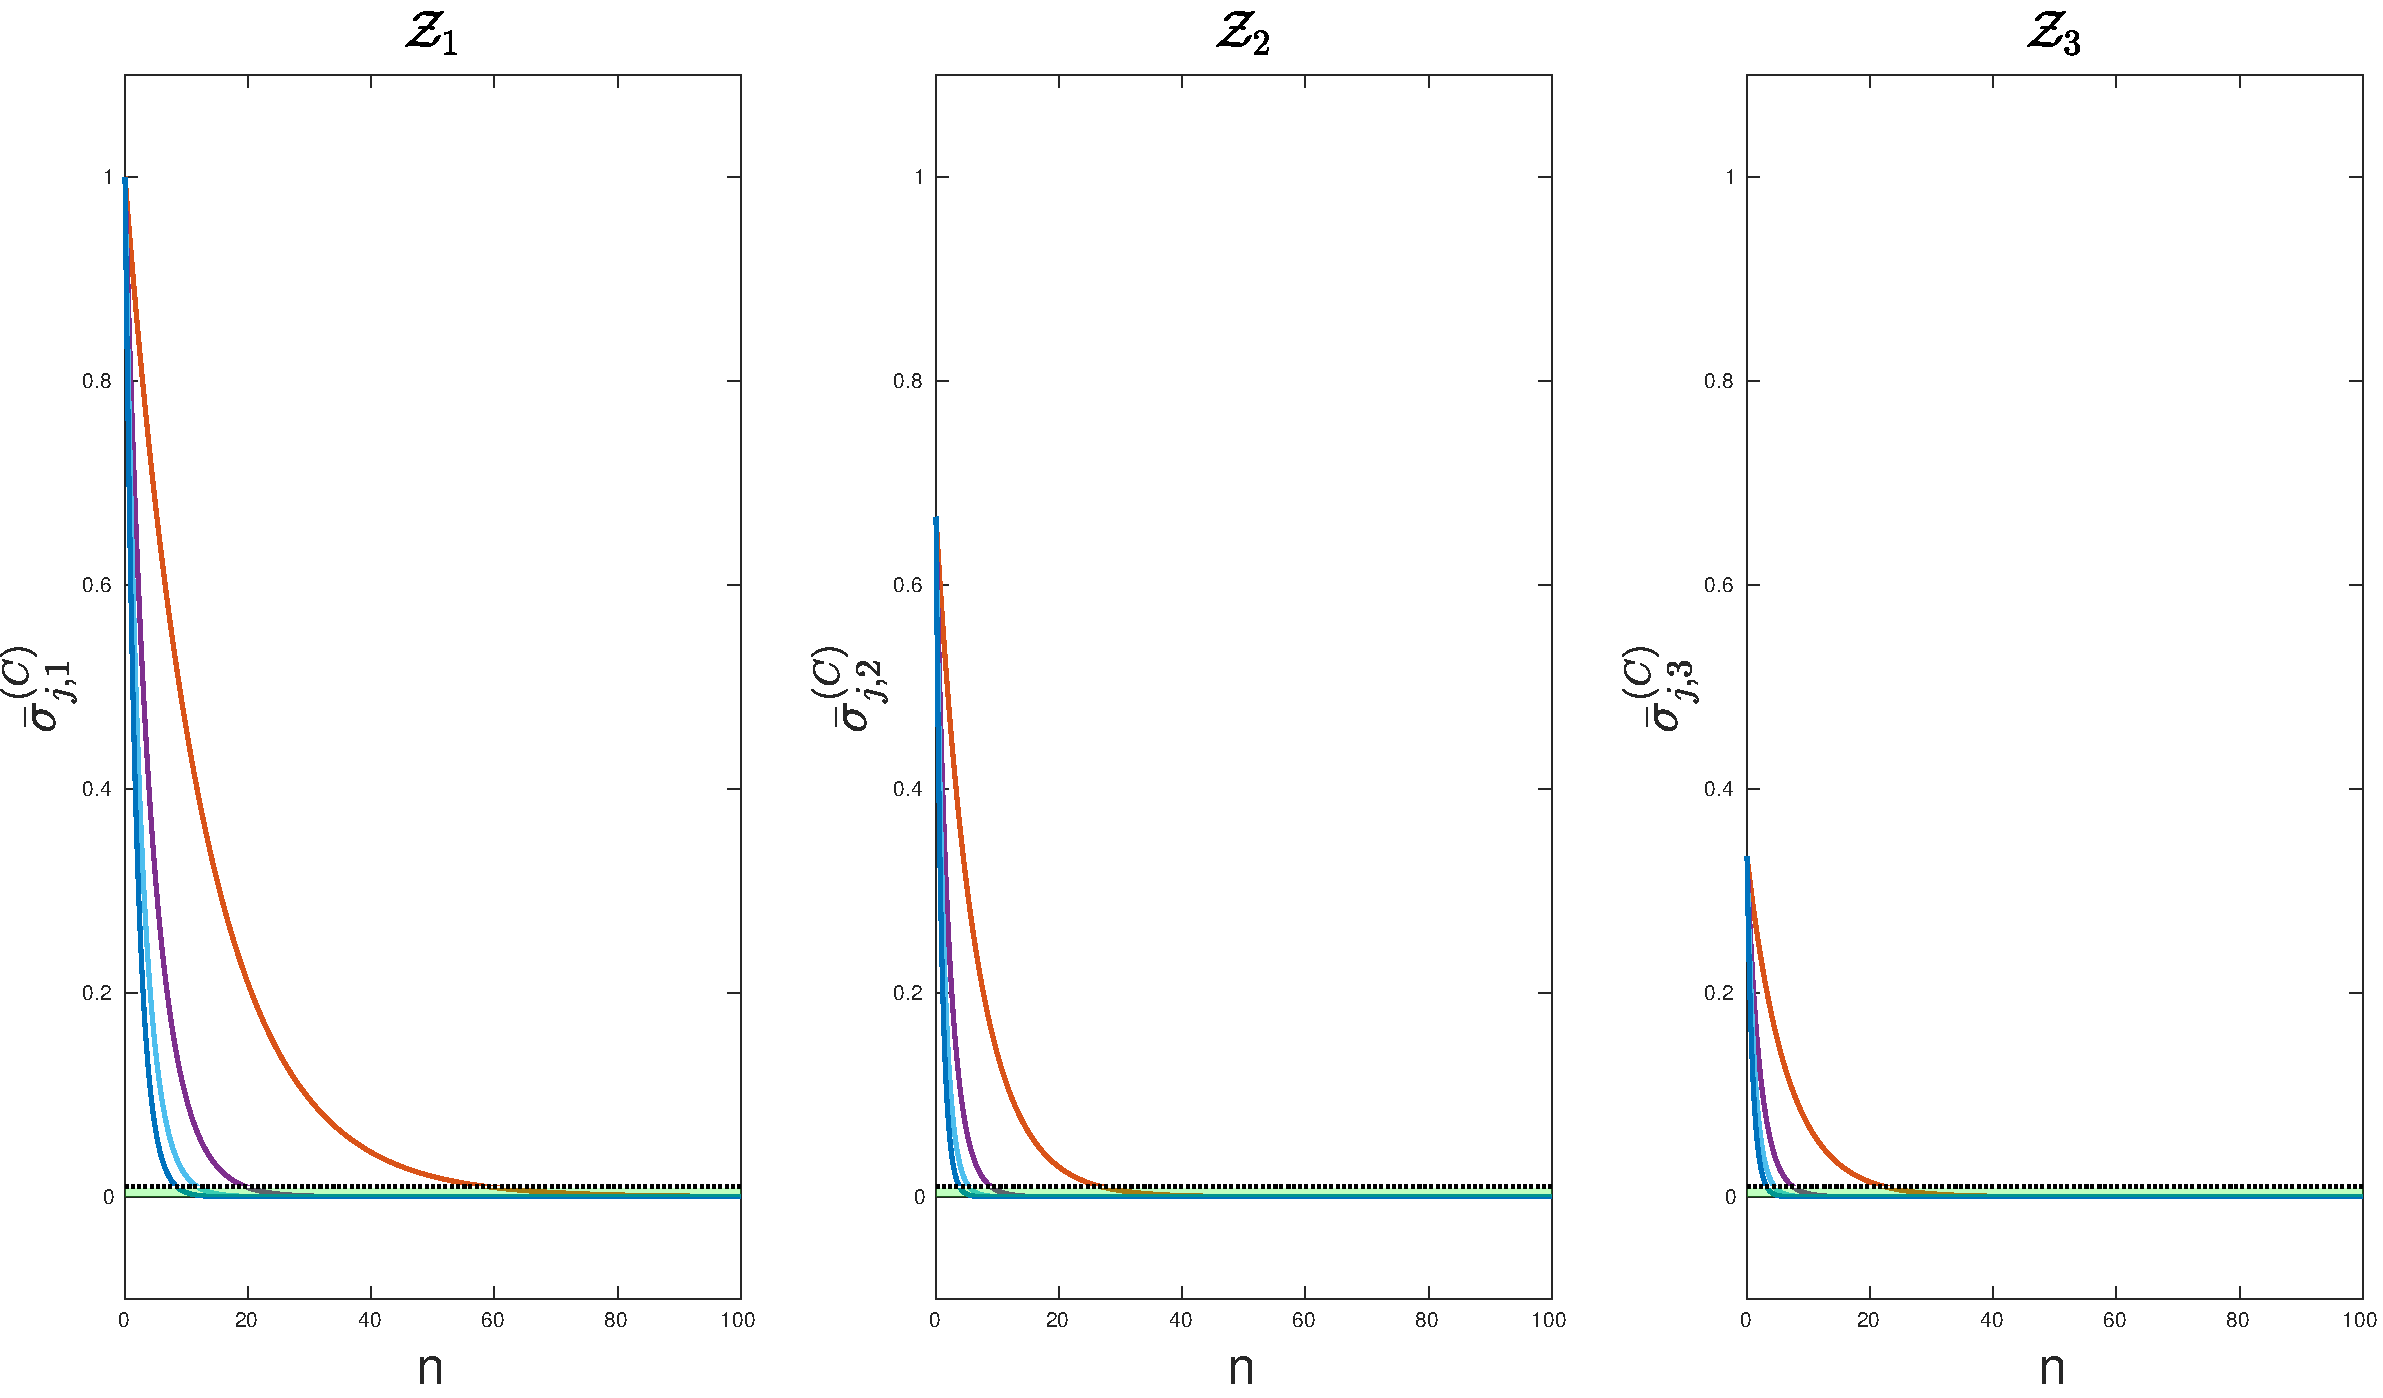
\includegraphics[width= 0.8\textwidth]{fig/dynamics_collective_learning.pdf} \label{fig:dynamics_collective_learning}}
	\hspace*{\fill}
	\caption[] {\label{fig:collective_learning} Scenario 1: \subref{fig:cluster_learning_sequence} the skills of each cluster are learned by the $ m$ robots in succession, \subref{fig:dynamics_isolated_learning} isolated learning,  \subref{fig:dynamics_incremental_learning} incremental learning,  \subref{fig:dynamics_incremental_transfer_learning} incremental + transfer learning, \subref{fig:dynamics_collective_learning} collective learning.}
\end{figure*}
% ---

% ===================================================================================================
\subsection{The skill complexity of the different paradigms}
The remaining knowledge for the four skills learned per robot are shown in Fig.~\ref{fig:collective_learning} in logarithmic scale. With the parameters discussed previously the $m$ robots are used to learn in parallel the $N_\mathcal{Z}$ skills of each cluster in succession, as shown in Fig.~\ref{fig:cluster_learning_sequence}. Notice that as expected, isolated learning (Fig.~\ref{fig:dynamics_isolated_learning}) exhibits the worst performance, always requiring $c_0$ episodes to learn every single skill. Since incremental learning (Fig.~\ref{fig:dynamics_incremental_learning}) does not benefit from the knowledge from the previously visited clusters, a robot $r_i$ needs to start accumulating knowledge from the beginning every time it moves to a different cluster. This is not the case in transfer learning (Fig.~\ref{fig:dynamics_incremental_transfer_learning}), as the more clusters a robot has visited the faster a new skill is learned. The speed of knowledge collection is clearly exponentiated with collective learning (Fig.~\ref{fig:dynamics_collective_learning}) thanks to the exchange of knowledge among the $m$ robots. In comparison to the other learning paradigms, with CL the skills are learned within a few trial episodes in every cluster. 

To assess how the number $m$ of robots affects the total number of trial episodes $C_\mathcal{S}$ required to learn all the $N_\mathcal{S}$ skills we use the same parameters as before but vary $m \in \left \lbrace 2,4,8,16,32,64,128\right \rbrace$. Moreover, we considered an additional collective learning scenario in which, unlike the previous case, the total number of available robots is distributed equally among the clusters to benefit from transfer learning at an earlier time during learning. The results are shown in Fig.~\ref{fig:total_episodes_per_n_robots}. From it, it can be seen that, at first, incremental learning is better than the trivial isolated learning case; however, as the number or robots increases, the skill knowledge is divided among the available robots which implies that less knowledge can be passed, as the pool of learned sills $\zeta_k$ per robot gets smaller. This explains why the total number of trial episodes for IsL and IL approach each other in the limit. TIL exhibits a similar behavior, as the number of robots grows, less cluster knowledge can be collected by each robot and transferred to the next cluster. Indeed, TIL rapidly converges to IL and eventually to IsL. In CL, a similar effect shows that when all robots are learning skills in from the same clusters, as the number of robots grows, the total complexity approaches that of the same number of robots distributed across clusters.
% ---
%\begin{figure}[!th]
%	\centering
%	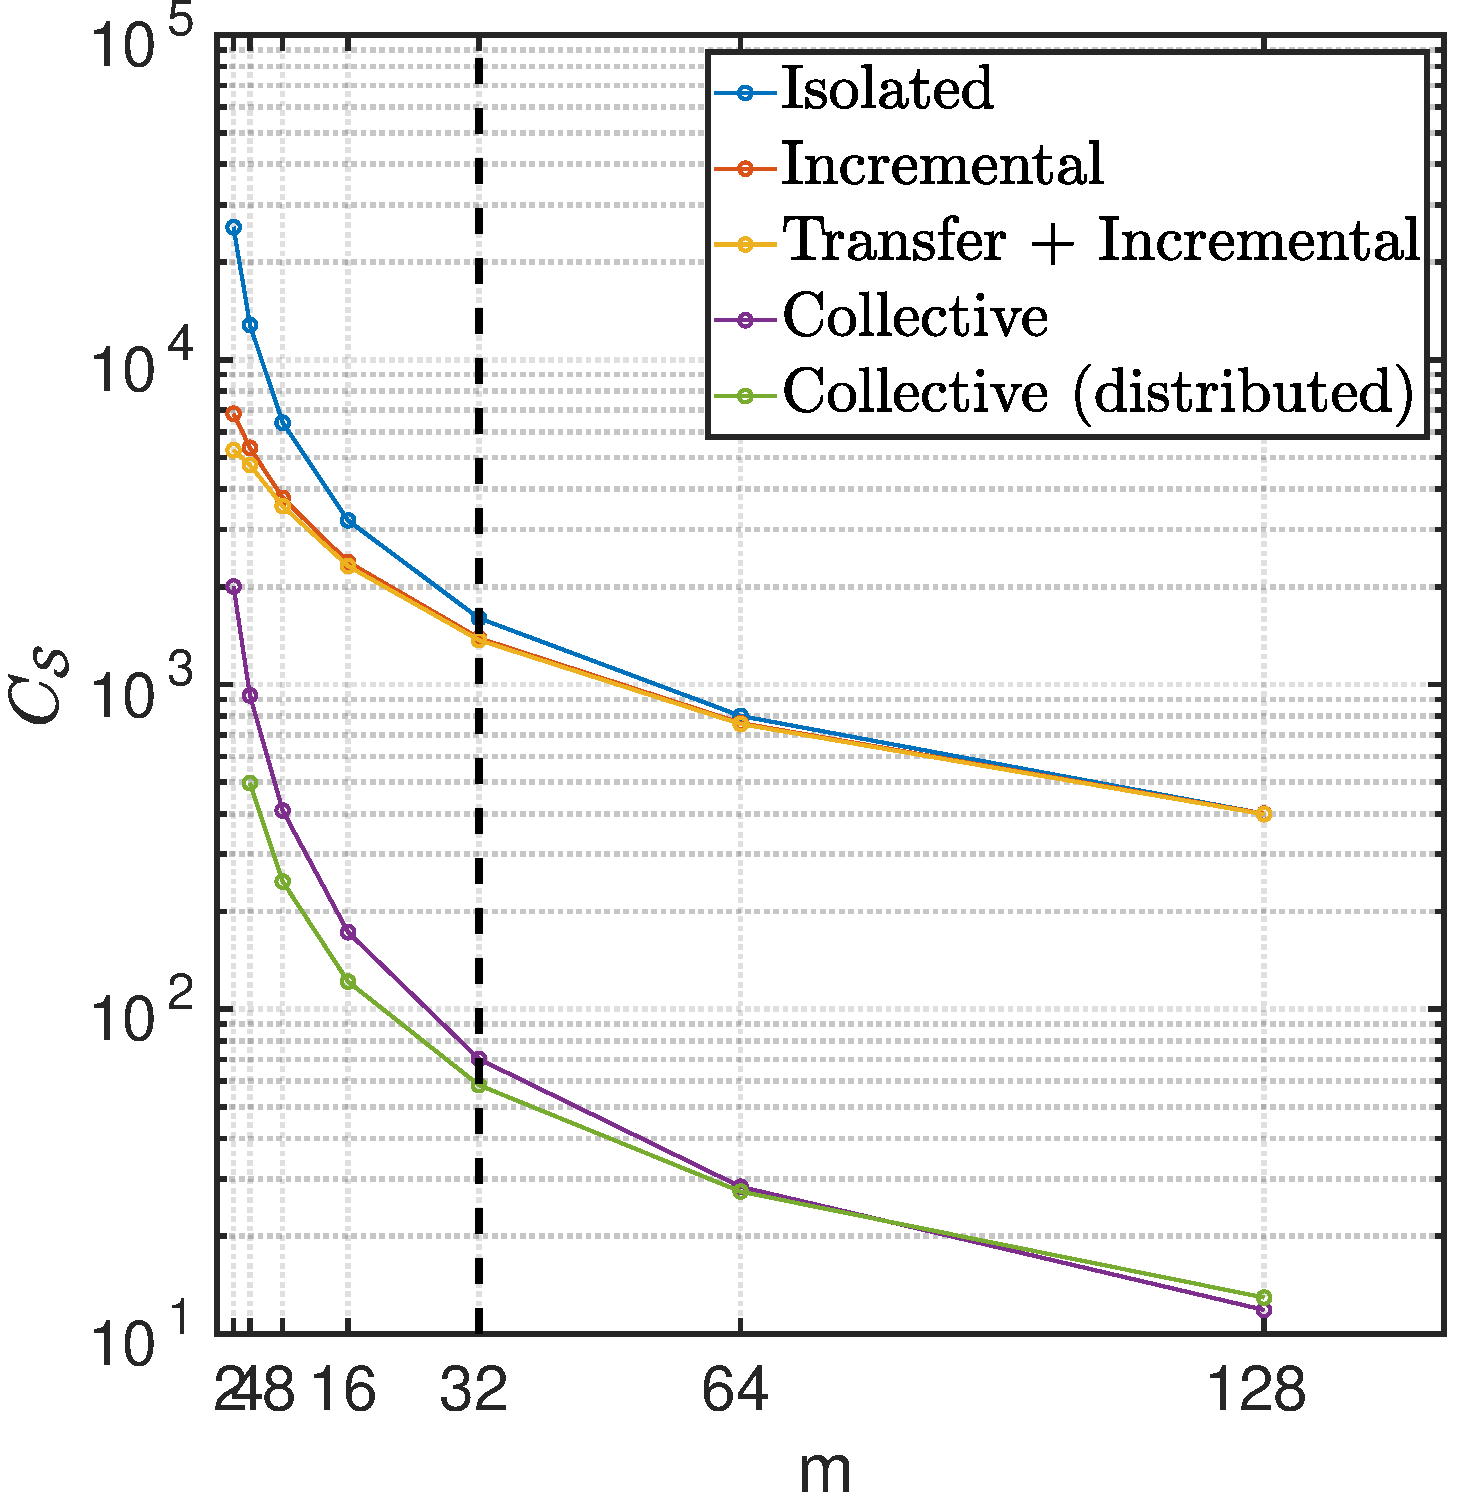
\includegraphics[width=0.9\columnwidth]{fig/total_episodes_per_n_robots.pdf}
%	\caption{Total number of episodes to learn the universe of skills as a function of the available robots.}
%	\label{fig:total_episodes_per_n_robots}
%\end{figure}
%% ---


% SUBSECTION ========================================================================================
\subsection{Energy consumption}
Consider that the results in \ref{fig:total_episodes_per_n_robots} shows the total number of episodes required by each of the $m$ robots. To compute the total energy demand those numbers need to be scaled by the factor $m e_0$, which leads to the consumption shown in Fig.~\ref{fig:total_energy_per_n_robots}.
% ---
%\begin{figure}[!th]
%	\centering
%	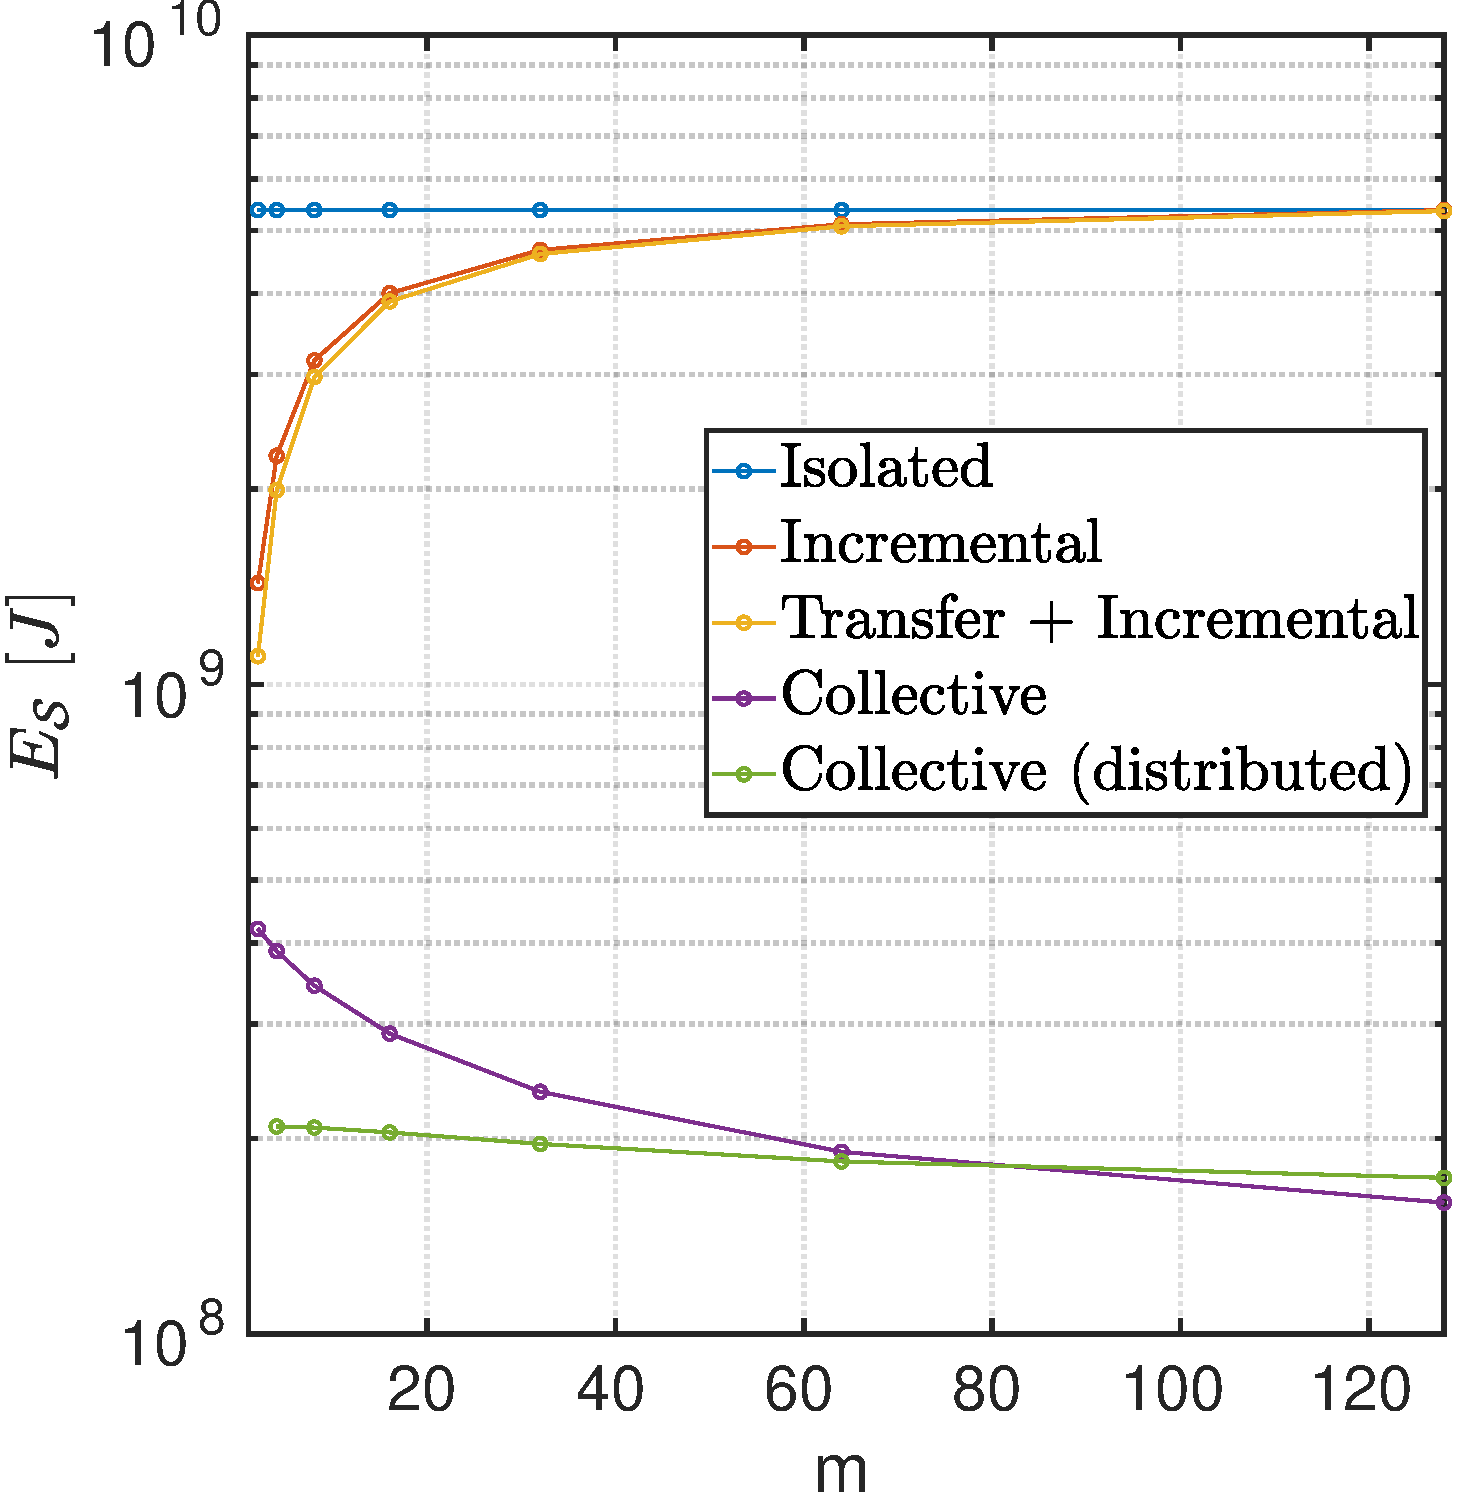
\includegraphics[width=0.9\columnwidth]{fig/total_energy_per_n_robots.pdf}
%	\caption{Total energy consumption.}
%	\label{fig:total_energy_per_n_robots}
%\end{figure}
%% ---

\begin{figure*}[!t]
	\centering
	\hspace*{\fill}
	\subfloat[]{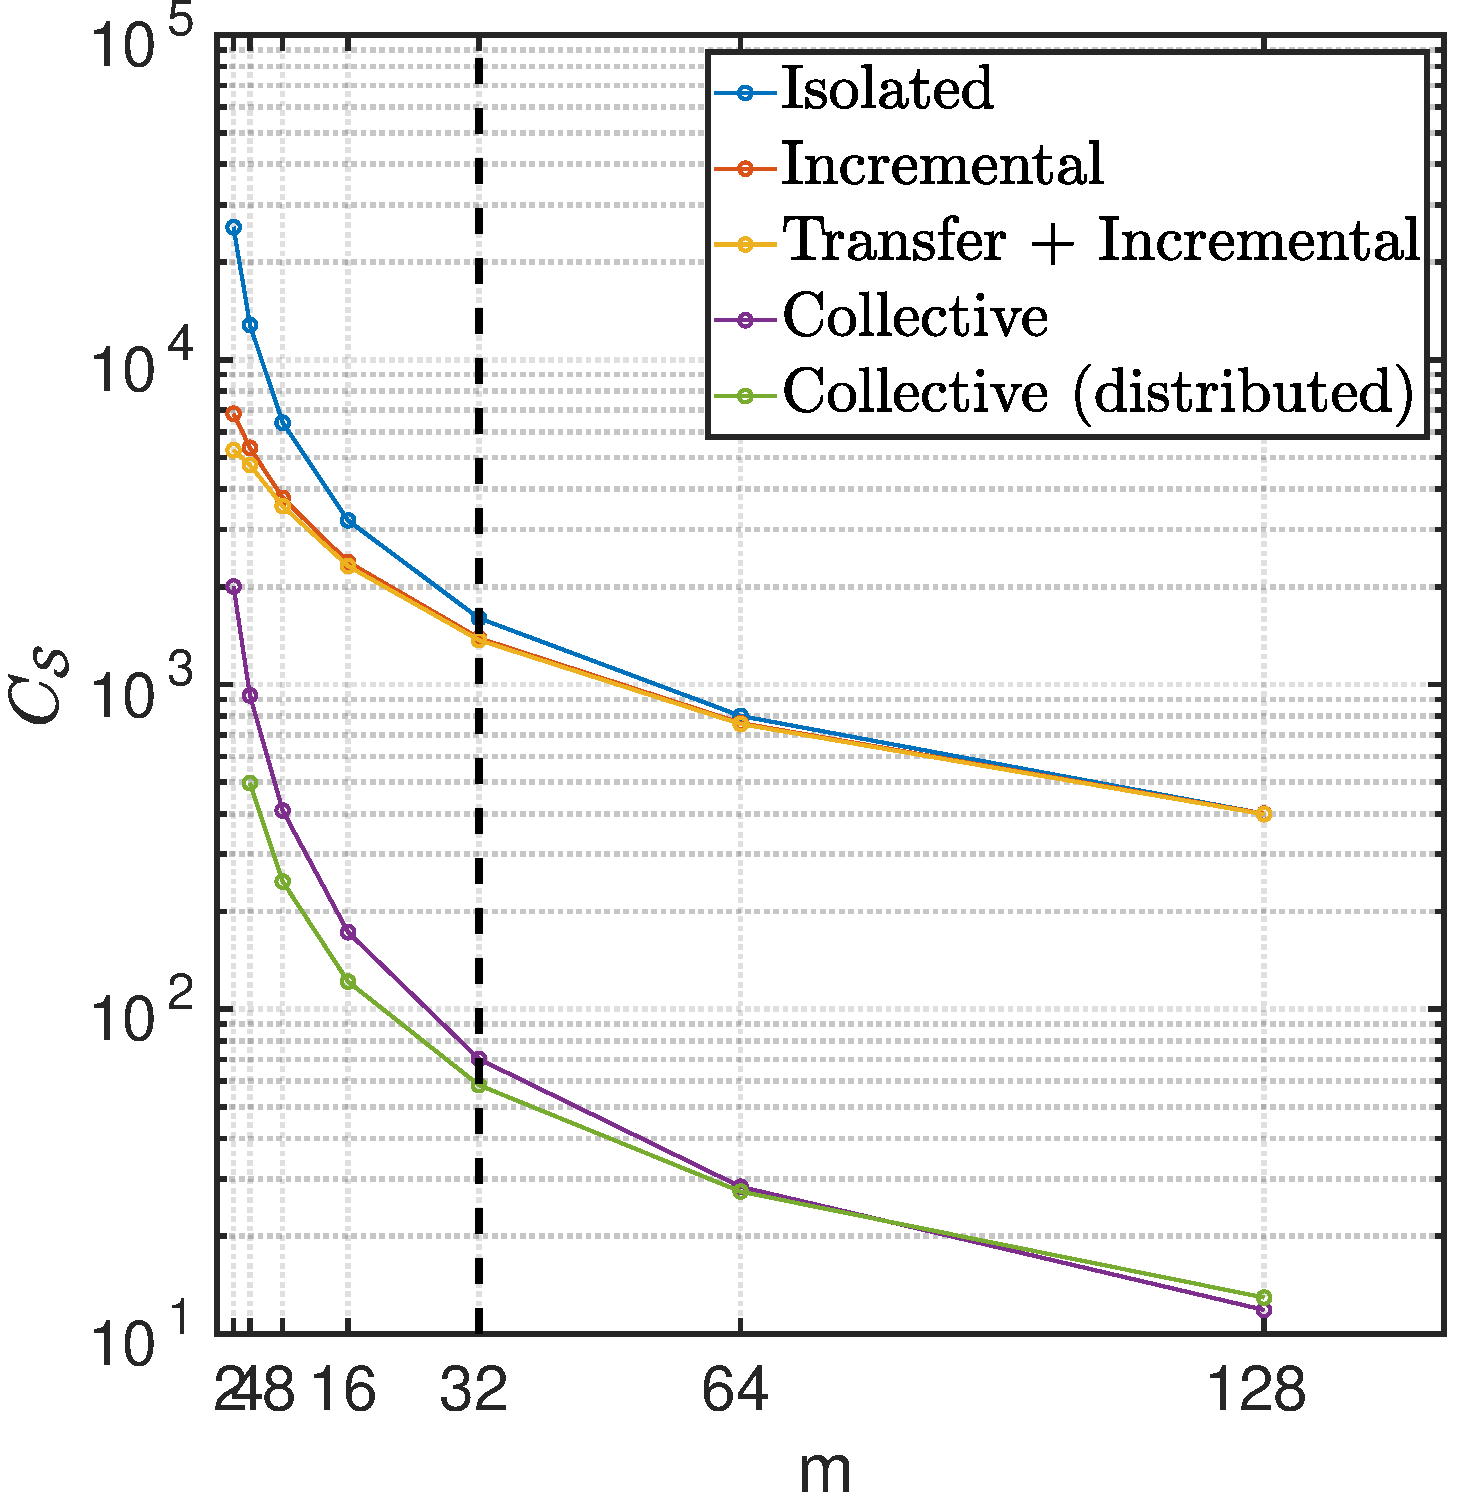
\includegraphics[width=0.45\textwidth]{fig/total_episodes_per_n_robots.pdf}
	\label{fig:total_episodes_per_n_robots}}  
	\hfill	
	\hspace*{\fill}
	\subfloat[]{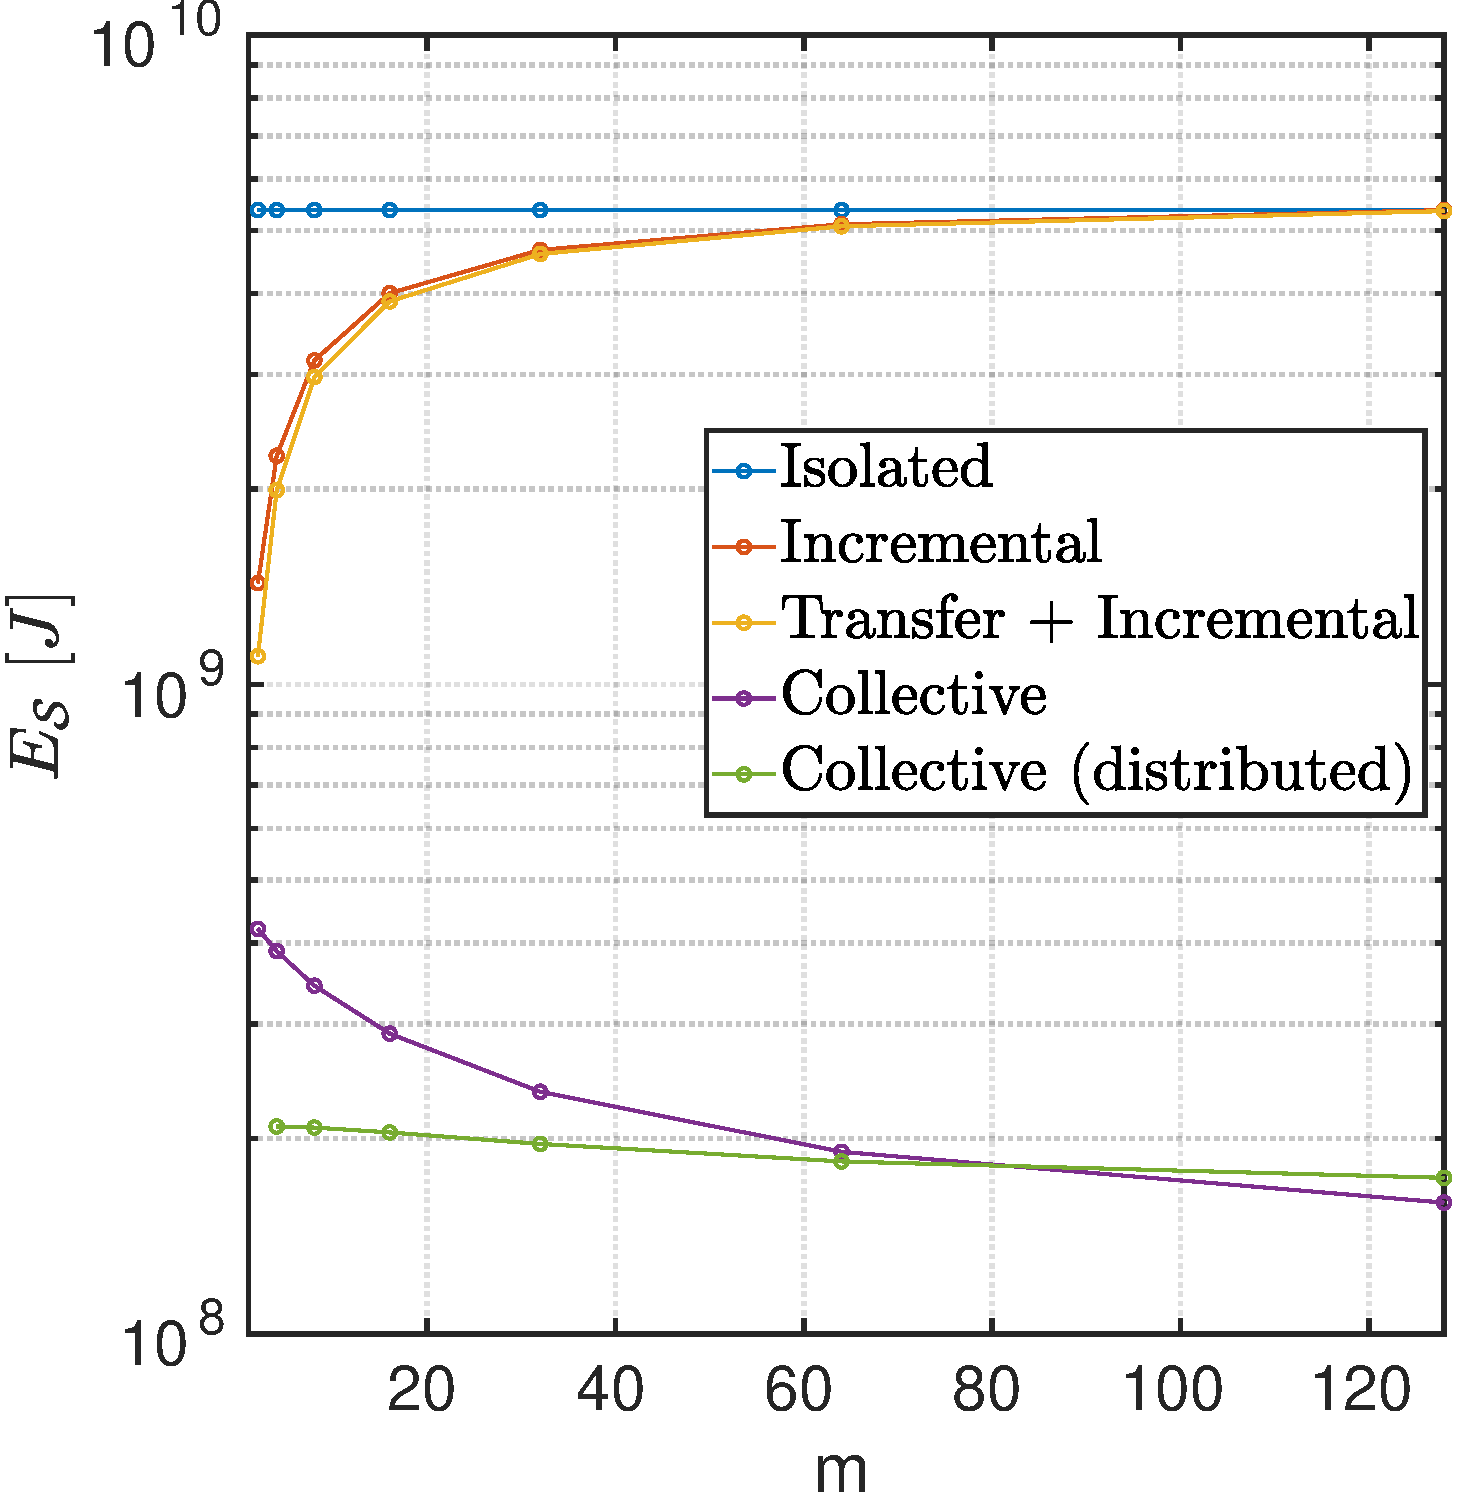
\includegraphics[width=0.45\textwidth]{fig/total_energy_per_n_robots.pdf}
	\label{fig:total_energy_per_n_robots}}
	\hspace*{\fill}
	\caption[] {\label{fig:final_results} The effect of the number of robots: \subref{fig:total_episodes_per_n_robots} Total number of episodes to learn the universe of skills as a function of the available robots and \subref{fig:total_energy_per_n_robots} the total energy consumption.}
\end{figure*}
% ---

Undoubtedly, collective learning shows that it has a not only the best energy usage of all the paradigms, but, inline the rest, the more robots are included the better energy usage. 

%Fig.~\ref{fig:iso_energy} shows the energy demand for a single task. Considering the parameters introduced above, we  estimate the energy and episodes needed by a single robot to learn all $N_{\mathcal{T}}$ tasks. For the episodes, we have
%% ---
%\begin{equation}¸
%    n^{Iso}_{\mathcal{T}} = N_{\mathcal{T}} \cdot c_j = 1,600\times 10 \times 100 = 1,600,000 \quad\text{episodes}.
%\end{equation}
%% ---
%With $P=\unit[1787.8]{W}$ and using \eqref{eq:energy_per_episode}-\eqref{eq:total_energy}. The total energy equates
%% ---
%\begin{equation}
%    E^{Iso}_{\mathcal{T}} = \unit[283.52]{GJ} %283,520,000,000.0,
%\end{equation}
%% % ---
% 
%% ---
%% SUBSECTION ========================================================================================
%\subsection{Incremental learning and transfer learning}
%%For ITL we consider a transfer factor of $\lambda=0.005$ to be used in \eqref{eq:similarity_metric}. Moreover, leveraging parallelization, $m=10$ robots learn $\frac{N_{\mathcal{T}}}{m} = 10$ tasks at the same time. 
%Then, using \eqref{eq:complexity_TIL}, \eqref{eq:itl_energy_per_task}, and \eqref{eq:itl_total_energy}; this results in the following episode and energy demands:
%% ---
%\begin{align}
%  n^{ITL}_{\mathcal{T}} &= 972,050\quad\text{episodes} \\
%  E^{ITL}_{\mathcal{T}} &= \unit[172.24]{GJ} % 172,247,385,965.70197
%\end{align}
%% ---
%% SUBSECTION ========================================================================================
%\subsection{Collective learning in the smart factory: a paradigm change}
%While incremental learning only takes the history of one robot into account, collective learning makes it able to use the already learned knowledge of all $m=10$ robots in the collective involved in the learning process. Using eqs. \eqref{eq:complexity_CL}, \eqref{eq:cl_energy_per_task} and \eqref{eq:cl_total_energy}; we obtain the following results,
%% ---
%\begin{align}
%  n^{ITL}_{\mathcal{T}} &= 106,119\quad\text{episodes} \\
%  E^{ITL}_{\mathcal{T}} &= \unit[18.80]{GJ} % 18,804,315,849.430477
%\end{align}
%% ---
%This represents energy savings of about $93 \%$ when compared to isolated learning coupled with drastic saving in time as the number of learning episodes reduces considerably. 
% 
%%  The results for the three schemes are summarized in Table~\ref{tab:results_summary}.
%% % ---
%% \begin{table}
%% \caption{Summary of the results for the learning schemes.\label{tab:results_summary}}
%%     \centering
%%     \begin{tabular}{c || c | c | c | c}
%%          & \multicolumn{2}{c|}{single robot} & \multicolumn{2}{|c}{multiple robots} \\
%%          & $E_{\mathcal{T}}\quad[GJ]$ & $n\quad [\#]$ & $E_\mathcal{T} [GJ]$ & $n \quad[\#]$ \\
%%         \hline
%%         \hline
%%         IL & $56.57$ & $160,000$ & $283.52$ & $1,600,000$ \\
%%         \hline
%%         ITL & --- & --- & $172.24$ & $972,050$ \\
%%         \hline
%%         CL & --- & --- & $18.80$ & $106,119$ \\
%%         \hline
%%     \end{tabular}
%% \end{table}
%% ---
%
%The energy demands as the number of learned tasks increases for all the considered learning schemes is shown in  Fig.~\ref{fig:use_case_results}. Evidently, collective learning reduces the energy consumption to the minimum in the least number of trial episodes. Furthermore, Fig.~\ref{fig:use_case_complexity} shows the scaled down complexities considering the parameters in \eqref{eq:transfer_constants}.
%


% ===================================================================================================
%                                                 |                                                 |
%                                                 |                                                 |
% -------------------------------------------- SECTION ---------------------------------------------|
%                                                 |                                                 |
%                                                 |                                                 |
% ===================================================================================================
\section{Conclusion}\label{sec:conclusion}
This work has presented arguments emphasizing energy consumption's significance in embodied AI systems. We introduced three principal categories of energy usage and juxtaposed them with the grand challenges stemming from the escalating population of Embodied AI (EAI) agents. It was underscored that mitigating energy consumption in EAI systems requires enhanced mechanical designs, efficient computational hardware and algorithms, and a paramount emphasis on harnessing the simultaneous sharing, exchange, transfer, and accumulation of knowledge acquired by the various EAI agents.

Our discussion on the established paradigms of isolated, incremental, and transfer learning showed that even with the deployment of multiple agents in parallel, optimal energy utilization remains unattainable in the absence of inter-agent knowledge exchange. Conversely, we established that the collective learning paradigm indeed presents a solution to the energy demand, contingent on the effective concurrent dissemination of knowledge based upon skill similarity. Indeed, our case study of a smart factory revealed a substantial escalation in energy requirements under conventional learning paradigms commensurate with the increasing use of EAI agents. In stark contrast, the collective learning approach demonstrated superior performance as robot numbers increased, which enables concurrently acquiring multiple skills knowledge.

We hope that our arguments will effectively focus the attention of the AI and robotics research community on the challenges arising from the emergence of EAI agents. Additionally, we expect that our discussion will foster the development of new machine-learning algorithms and communication methodologies that enable the rapid realization of collective learning strategies.

% ===================================================================================================
%                                                 |                                                 |
%                                                 |                                                 |
% -------------------------------------------- SECTION ---------------------------------------------|
%                                                 |                                                 |
%                                                 |                                                 |
% ===================================================================================================
\printbibliography

% ===================================================================================================
%                                                 |                                                 |
%                                                 |                                                 |
% -------------------------------------------- SECTION ---------------------------------------------|
%                                                 |                                                 |
%                                                 |                                                 |
% ===================================================================================================
\newpage
\section*{Appendices}
\begin{appendices}
	
% ===================================================================================================
%                                                 |                                                 |
%                                                 |                                                 |
% -------------------------------------------- SECTION ---------------------------------------------|
%                                                 |                                                 |
%                                                 |                                                 |
% ===================================================================================================
\section{Industrial robot energy consumption support data}\label{sec:app_robot_ener_consumption}
According to \cite{montaqim2015} and available press releases of different robotic companies \cite{fanuc2015, yaskawa2014, ABB2015}, the approximate distribution of the industrial robot install base per manufacturer is shown in Fig.~\ref{fig:manufacturers_pie}.
% ---
\begin{figure}[!ht]
	\centering
	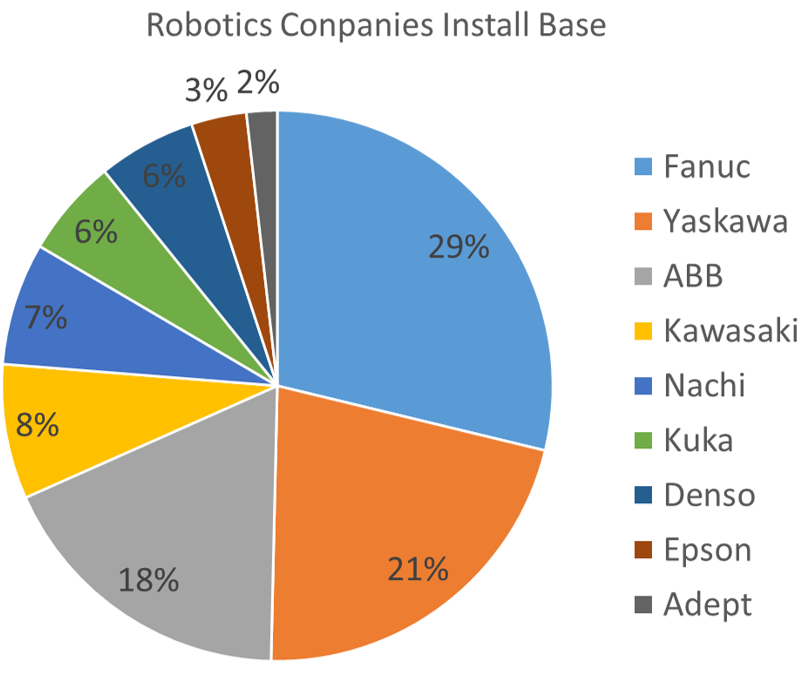
\includegraphics[width=0.95\columnwidth]{fig/manufacturers}
	\caption{Percentage of installed industrial robots per manufacturer}
	\label{fig:manufacturers_pie}
\end{figure}
% ---
Since Fanuc, Yaskawa, and ABB make for two-thirds of the total install base of industrial robots, we took the power consumption of the robots from those manufacturers to estimate the total power consumption. 
After surveying the datasheets for their robot portfolio, the average power consumption for each model was estimated. Additionally, every manufacturer classifies their robots according to one or more possible applications, which can be grouped into the application categories defined by the IFR. The average power consumption was calculated for every application using the values reported in the robot datasheets. Finally, the power consumption for each category was computed as a weighted average based on the companies' market share percentage (assuming that 68 \% is the total number of robots)\footnote[1]{These numbers should be used with discretion since there is no available information on which are the most common installed robot models. This information may change the estimation.}. The estimated power consumption per robot application is shown in Fig.~\ref{fig:ir_average_power}.
%---
\begin{figure}[h]
	\centering
	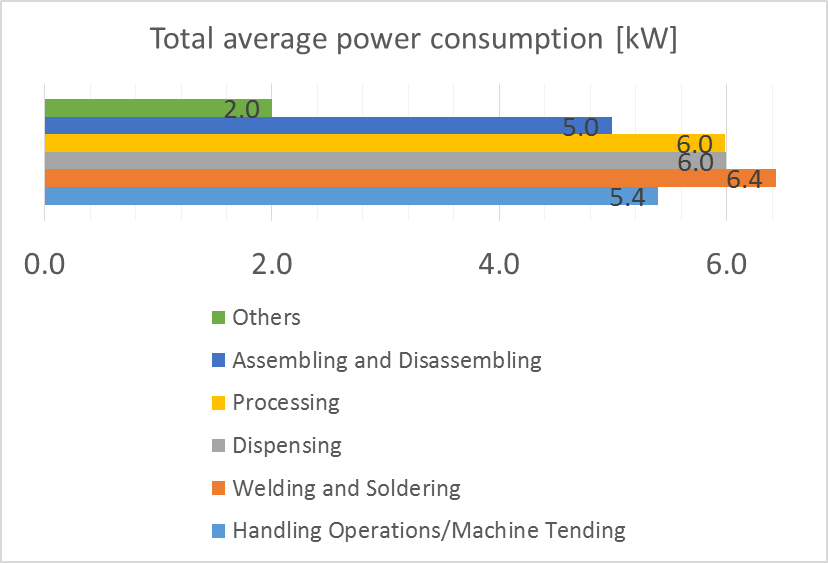
\includegraphics[width=0.95\columnwidth]{fig/industrial_robots_average_power_per_category}
	\caption{Average power consumption of industrial robots per category.}
	\label{fig:ir_average_power}
\end{figure}
%---
Using these numbers and the estimated operational stock of industrial robots reported in \cite{statista_ir_operational_stock} and by the International Federation of Robotics (see Fig.~\ref{fig:ir_stock}), the estimated worldwide industrial robot energy consumption was computed and shown in Fig.~\ref{fig:ir_energy}.
% ===================================================================================================
%                                                 |                                                 |
%                                                 |                                                 |
% -------------------------------------------- SECTION ---------------------------------------------|
%                                                 |                                                 |
%                                                 |                                                 |
% ===================================================================================================
\section{Collaborative robots}\label{sec:app_cobot_ener_consumption}
To approximate the energy consumption of cobots we looked at the power consumption per payload of various manufacturers, see Fig.~\ref{fig:cobot_watt_per_kg} resulting in an average power consumption of approximately 40 W. Together with a typical power consumption of the robot controller of 60 W \cite{Heredia2023BreakingEnergyConsumption}, we consider a total of 100 W power demand. Similar to the industrial robots, the worldwide energy consumption was calculated assuming a 24/7 operation.
%---
\begin{figure}[h]
	\centering
	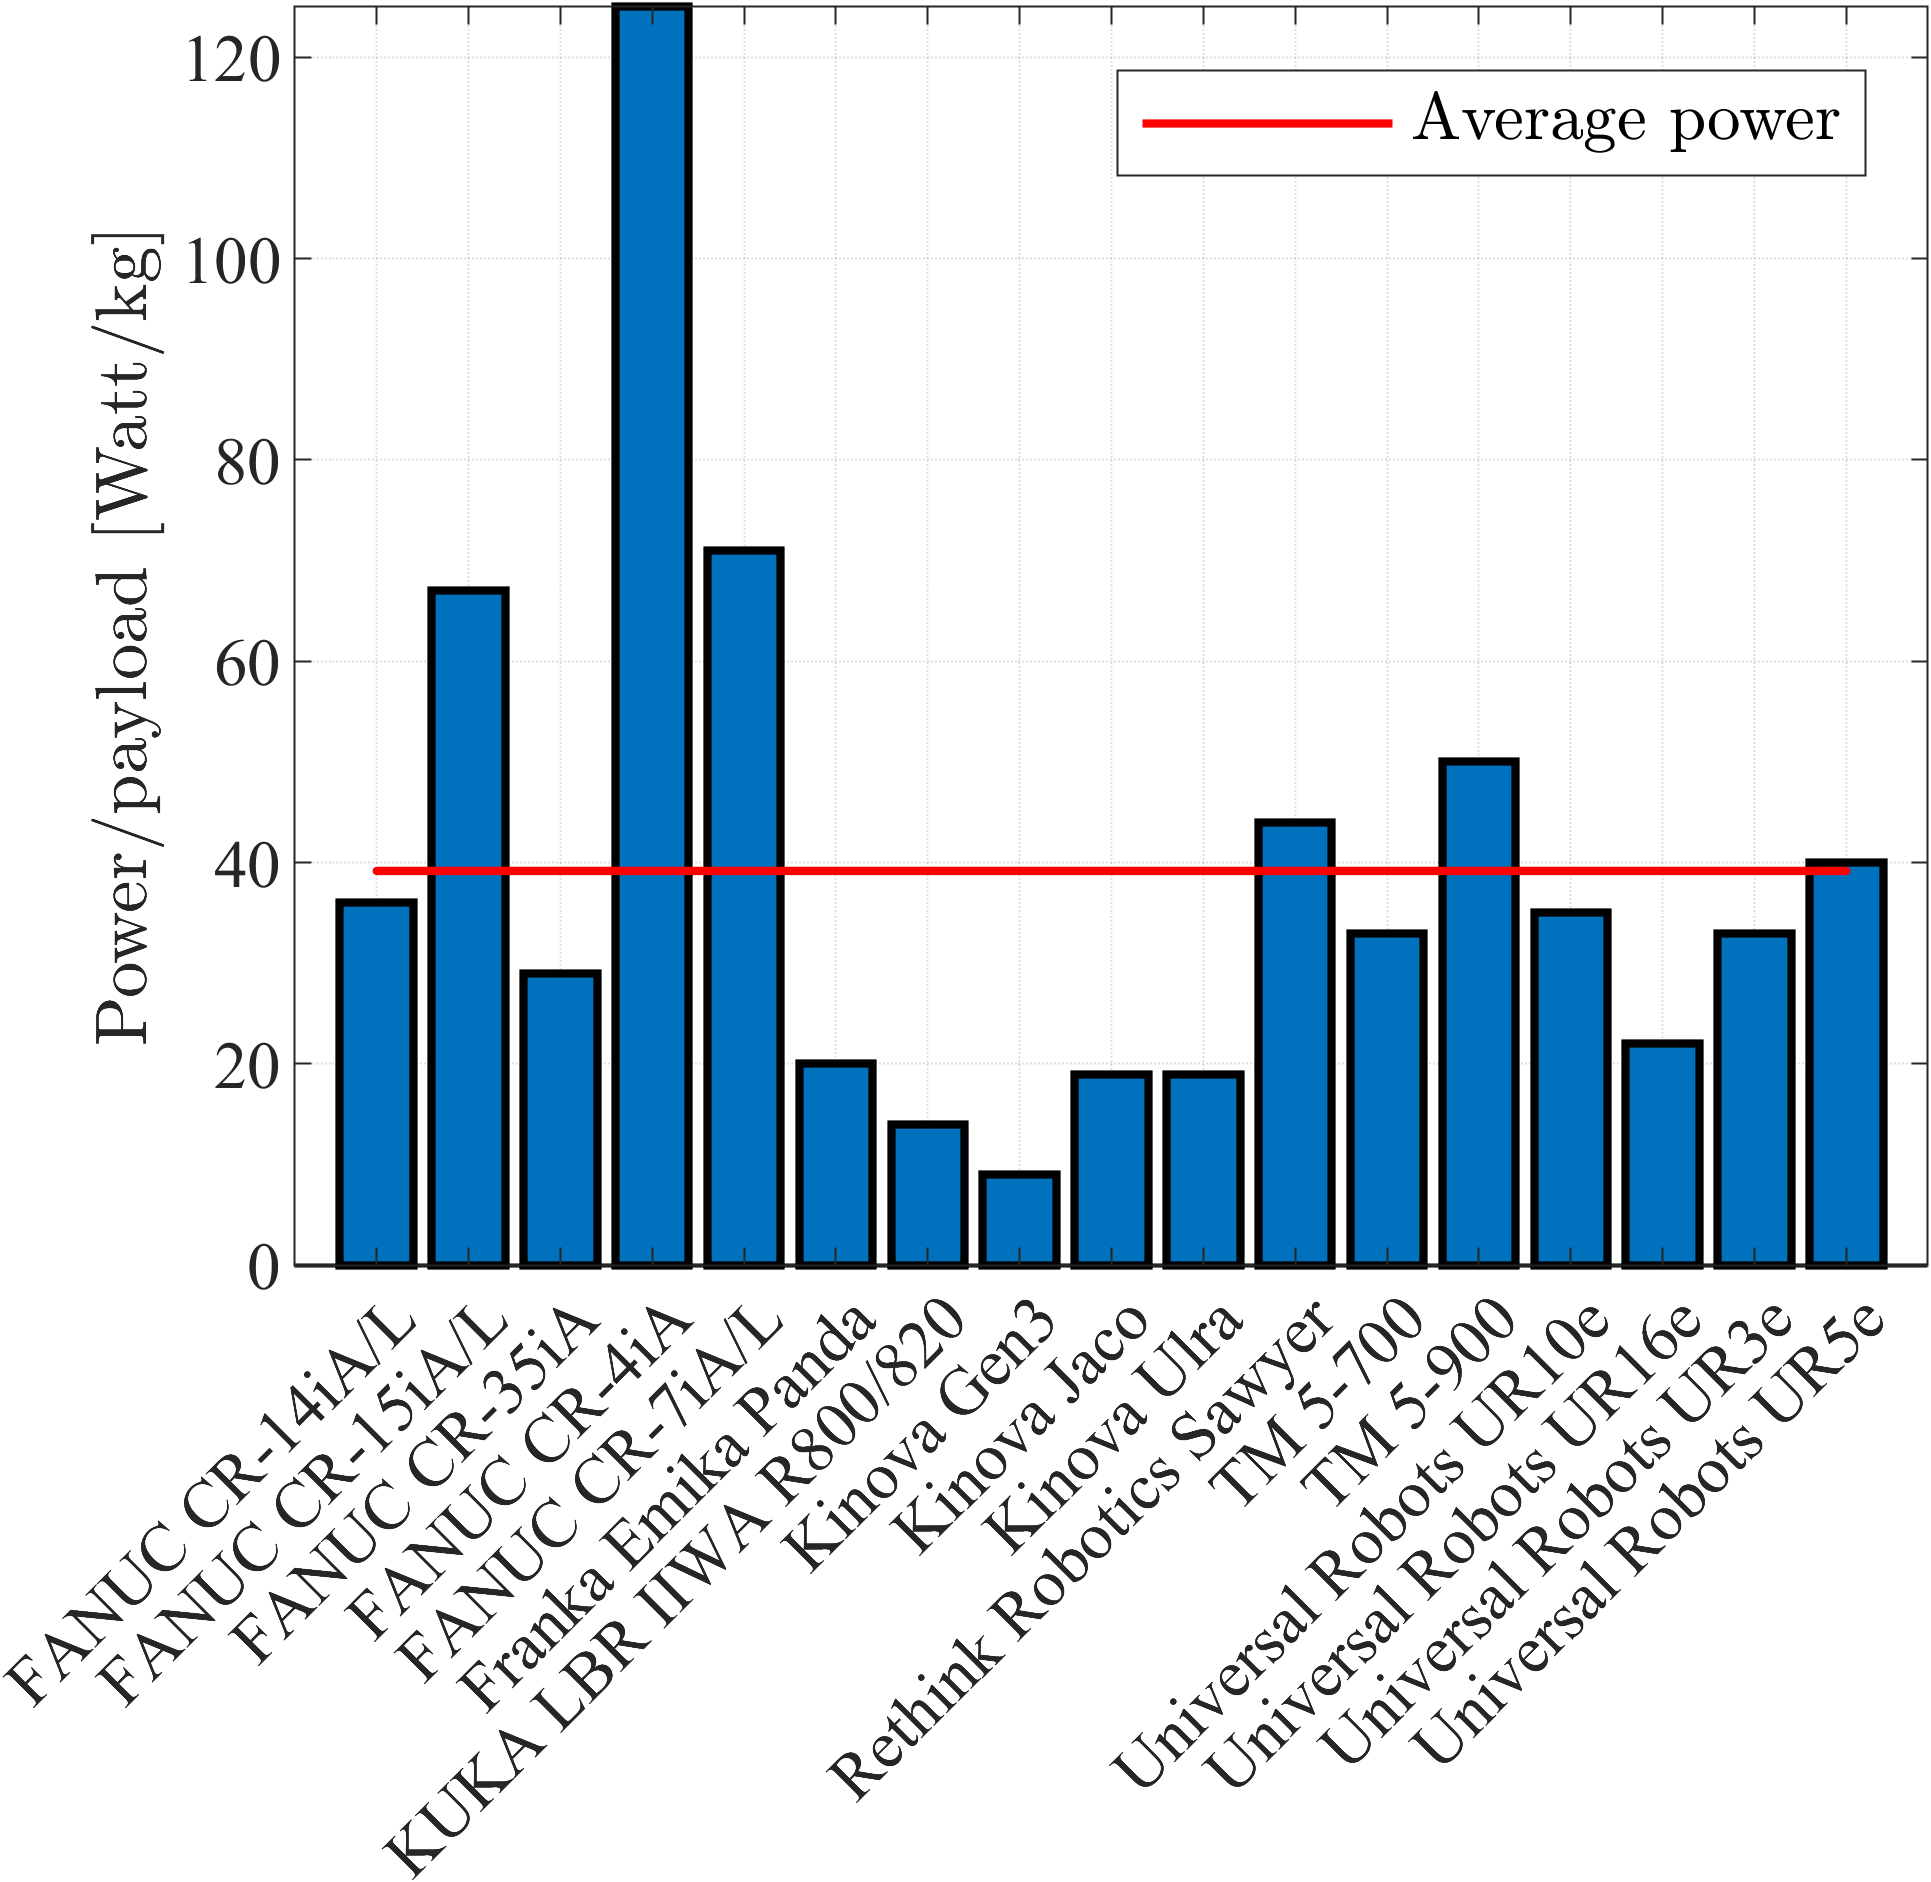
\includegraphics[width=0.95\columnwidth]{cobot_watt_per_kg.png}
	\caption{Power consumption per payload for different cobots.}
	\label{fig:cobot_watt_per_kg}
\end{figure}
%---

\end{appendices}




\end{document}